\documentclass{report} % Add the document class
\usepackage{graphicx} % For including graphics like logos
\usepackage{subcaption}
\usepackage{lipsum}   % For dummy text
\usepackage{setspace} % For line spacing
\usepackage{fancyhdr} % For custom headers and footers
\usepackage{geometry} % For page margins
\usepackage{amsmath} % For mathematical equations
\usepackage{enumitem} % For customized lists
\usepackage{amsfonts} % For the \forall symbol
\usepackage{multicol} % For multiple columns if needed
\usepackage{hyperref} % For hyperlinks for table of contents
\usepackage{acronym} % For defining acronyms
\usepackage{tocbibind} % For adding list of figures, tables to table of contents
\usepackage{tabularx} % For tables
\usepackage{float} % For tables
\usepackage{longtable}%to split tables over multiple pages
\usepackage{array}
\usepackage{booktabs}
\usepackage{caption}
\usepackage{hyperref}
\usepackage{fancyheadings}
\usepackage{multirow}
%
\pagestyle{fancy}
\fancyhead[R]{
    
\includegraphics[width=0.1\textwidth]{./ReportImages/thws_logo.png} % Adjust path and filename
}
\fancyhead[C]{} 
\fancyhead[L]{} 
\addtolength{\headwidth}{\marginparsep}
\addtolength{\headwidth}{\marginparwidth}

\geometry{top=1in, bottom=1in, left=1in, right=1in} % Set page margins

% Configure the hyperref package to remove red boxes and customize link colors
\hypersetup{
    colorlinks=true,      % Set to true to enable colored links
    linkcolor=black,       % Color for internal links (sections, pages, etc.)
    citecolor=black,       % Color for citation links
    filecolor=black,       % Color for file links
    urlcolor=black         % Color for URL links
}


\begin{document}

% Title Page
\begin{titlepage}
    \centering
    \vspace*{1cm}
    
    \Large \textbf{Technical University of Applied Sciences Würzburg-Schweinfurt (THWS)}\\
    \vspace{0.5cm}
    \Large Faculty of Computer Science and Business Information Systems\\
    \vspace{1cm}
    
    \huge \textbf{Master Thesis}\\
    \vspace{1.5cm}
    
    \Huge \textbf{Electrical Engine Efficiency Prediction Bypassing Finite Element Analysis}\\
    \vspace{2cm}
    
    \large \textbf{Submitted to the Technical University of Applied Sciences Würzburg-Schweinfurt in the Faculty of Computer Science and Business Information Systems to
    complete a course of studies in Master of Artificial Intelligence}
    
    \vspace{1cm}
    
    \huge Lilly Abraham\\
    \huge K64889\\
    \vspace{1cm}
    \large Submitted on: 11.12.2024\\
    
    \vfill
    
    \large
    Initial examiner: Prof. Dr. Magda Gregorová\\
    Secondary examiner: Prof. Dr.-Ing. Mercedes Herranz Gracia\\

\end{titlepage}

\newpage 
\begin{figure}[h]
    \centering
    
\includegraphics[width=0.5\textwidth]{./ReportImages/qrcode.png} 
    \label{fig:qrcode}
\end{figure}

\chapter*{Abstract}
\addcontentsline{toc}{chapter}{Abstract}

The thesis explores an approach to predict Key Performance Indicators (KPI)s of topology invariant Permanent Magnet Synchronous Machine
(PMSM) Electric Motors from its geometric, physical and simulation parameters.
I intend to model the dynamics of Electric Motor functionality by creating surrogate models trained with Finite Element Method (FEM) simulations from its parametric description.
The KPIs to be predicted are vectors of numerical values which can be displayed as the Torque curve(2D) and the Efficiency grid(3D) respectively.
I note the relationship between the Torque curve and the Efficiency grid and incorporate my learnings of both the KPIs nature into the solutions's modelling.
I first parameterize the Electric Motor design such that it is feasible to convert into a tabular representation.
Next, I create a table with relevant attributes and design a Multi Linear Perceptron(MLP) to train it in a supervised manner.
Subsequently I regularize the loss functions in a way that would smoothen out the plot curves for both the KPIs.
Then I evaluate the predictions with the test target values by experimenting with various hyperparameter tuning settings 
and as a baseline with the average of the parameters.
Additionally I conduct a study to model the task as its graph representation and use Graph Neural Networks(GNN) to predict the KPIs.
Lastly I enable the KPIs plot visualization in a manner presentable to the client Valeo(Automaker Company specializes in  electric motors for cars).

\chapter*{Acknowledgement}
\addcontentsline{toc}{chapter}{Acknowledgement}
I would like to thank my supervisor Prof. Dr. Magda Gregorová for her guidance and support throughout the course of this thesis.
Her dedication and commitment to our work has been inspiring to me notably on how I transformed statistical math into modelling that I might have developed a 
new love for academia. I would also like to express my sincere gratitude to Valeo for providing us with the dataset.
Special thanks are in order to Daniel and Leo for sharing valuable insights of the data from an electromechanical standpoint and for giving me a detailed understanding 
of my task. I owe my accomplishments to my Family who have been very instrumental in making it possible for me to pursue a Master's degree outside my home country 
and their endless support throughout enabled me to get to my thesis moving in the right direction. Finally, I humble myself before God Almighty for all his blessings 
and for giving me the strength to persevere and bring my dreams to fruition.

\begin{spacing}{1.2}
    \tableofcontents
\end{spacing}

\chapter*{Abbreviations}
\addcontentsline{toc}{chapter}{Abbreviations}
\begin{acronym}[TDMA]
  
    \acro{GNN}{Graph Neural Network}
    \acro{MLP}{Multi Linear Perceptron}
    \acro{KPI}{Key Performance Indicator}
    \acro{EM}{Electric Motor}
    \acro{FEA}{Finite Element Analysis}
    \acro{CNN}{Convolution Neural Network}
    \acro{D}{Dimensional}
    \acro{MSE}{Mean Squared Error}
    \acro{RMSE}{Root Mean Squared Error}
    \acro{NaN}{Not a Number}
    \acro{ReLU}{Rectified Linear Unit}
    \acro{GPU}{Graphics Processing Unit}
    \acro{MP}{Message Passing}
    \acro{PDE}{Partial Differential Equation}
    \acro{PMSM}{Permanent Magnet Synchronous Machine}
    \acro{ANN}{Artificial Neural Network}
    \acro{GCN}{Graph Convolutional Network}

\end{acronym}

\newpage

\newpage

\chapter{Introduction} 
In the design of \ac{PMSM} \ac{EM}, vast amounts of data are generated to determine which design of an \ac{EM} fits best to \ac{KPI}s.
Traditionally these \ac{KPI}s are inferred from the description of an \ac{EM} design using \ac{FEA} simulations by approximating the solutions of the Maxwell's equations 
which are essentially \ac{PDE}.
WRITE MORE..ATTRACT THE READER \\

\ac{KPI}s of an \ac{EM} are representative characteristics of a motor drive and is essential to judge the performance of the motor before manufacturing it.
The Torque multiplied by the Angular Velocity gives us an insight of the total Power of the \ac{EM}.
The Efficiency map is a behavior map that expresses the motor efficiency function in the torque-angular velocity domain of an \ac{EM}.
One would calculate such kind of behavior maps when there are multiple operating points to consider within the \ac{EM}'s drive cycle.
The other \ac{KPI}s such as Losses and Torque ripple are also behavior maps similar to the Efficiency \ac{KPI}.
The paper in Ref. \cite{ETA-2021} also cites that the Efficiency vs Torque and Angular Velocity map is most representative of the characteristics of the \ac{EM}.  \\

\ac{FEA} are numerical methods that discretize any physical phenomena to simulate and understand its performance under given loads and boundary conditions during design 
phase. This enables designers to understand the performance and make a well informed decision on manufacturing it. Although \ac{FEA} only gives approximate solutions, 
it is regarded the best among the alternatives that exists.
\ac{FEA} as a method are used in several domains ranging from civil, mechanical, aerospace, automotive and electrical engineering to name a few.

\begin{figure}[H]
    \centering
    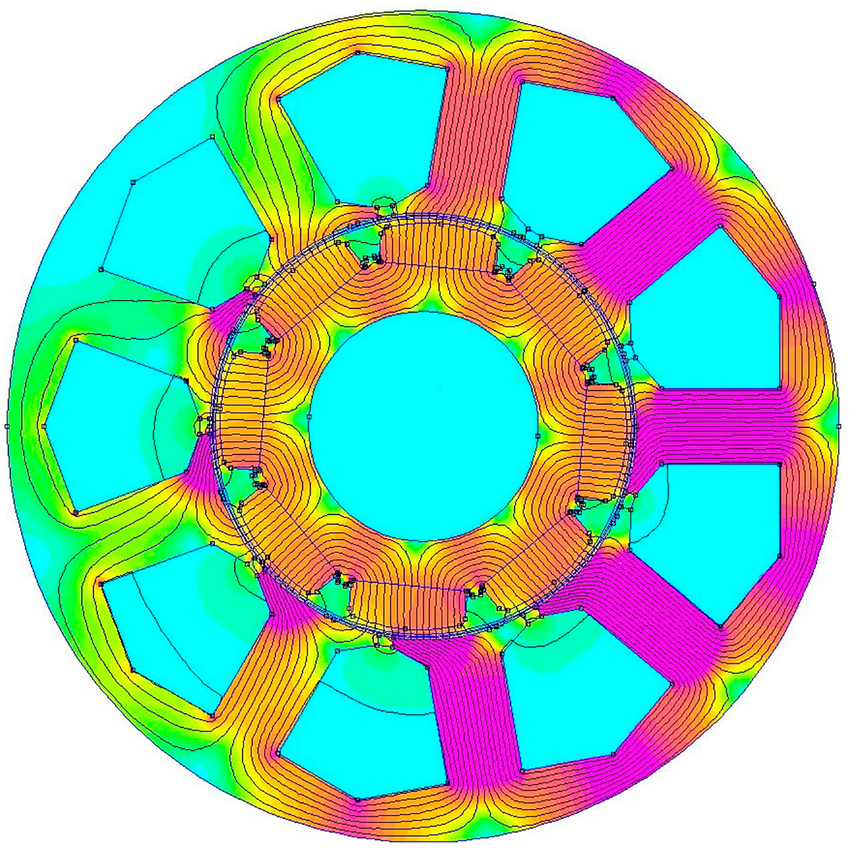
\includegraphics[width=0.35\textwidth]{./ReportImages/FEA.png} 
    \caption{\ac{FEA} Simulation of a \ac{PMSM} (Source : \cite{CNNFEA-2020})}
    \label{fig:FEA Simulation of a PMSM}
\end{figure}

Fig. \ref{fig:FEA Simulation of a PMSM} represents an \ac{FEA} discretized mesh of a \ac{PMSM} motor.READ PAPER TO CLARIFY EXACTLY WHAT KIND OF MOTOR
The color scale obtained in  represents possibly the magnetic flux density flowing across different parts of the \ac{EM}.

\ac{FEA} simulations here discretize the geometric parameters of an \ac{EM} into finite elements.
The simulations are then carried out by creating a mesh with the discretized points that approximate the shape of the \ac{EM} and then solving the \ac{PDE}s for each of them.
This is typically done to simulate the magnetic field distribution of the \ac{EM} and thus assists to generate its \ac{KPI}s.  
It requires domain knowledge in motor physics and complicated setup to run simulations typically in \texttt{Matlab}\footnote{\url{https://de.mathworks.com/}}.
Moreover, \ac{FEA} simulations are famously expensive in terms of time taken to solve the equations which are also non differentiable.
Despite the computational burden it comes with, the authors from Ref. \cite{FEA-ETA-2017} defends \ac{FEA} to be most appropriate to 
generate \ac{EM} efficiency maps in terms of accuracy based on experimenting overall error rates across operating ranges for different \ac{EM} losses.\\

\ac{FEA} though well established in the \ac{EM} design is very resource intensive, time consuming and does not allow for high-throughput engine design optimization. 
Hence, the growing need to replace it with a worthy substitute.
Deep learning can be seen as the most eligible surrogate of \ac{FEA} simulator as they can provide almost accurate results in relatively no time. 
Particularly for the Efficiency \ac{KPI}, \ac{FEA} simulations may take hours to days as it needs to generate for all operating points in the Efficiency map.
\ac{FEA}-based \ac{ANN} models have been utilized in other applications such as for predicting stress distribution in 3D printing, bend angles in laser-guided bending, 
and performance of thermoelectric generator as cited in Ref. \cite{SM EMT-2020}.\\

The actual engine data of \texttt{Valeo}\footnote{\url{https://www.valeo.com/}} is used here as the dataset comprising of multiple variant designs of the Double-V 
magnet \ac{EM} topology. Valeo is an Automaker company that specializes in manufacturing electric motors for automobiles.\\
Fig. \ref{fig:Valeo Motor Structure} depicts the structure of an \ac{EM} manufactured by Valeo. 
The rotor rotates around the Stator to produce the magnetic field whereas the Stator is the stationary part that generates the force to rotate the Rotor.         
\begin{figure}[H]
    \centering
    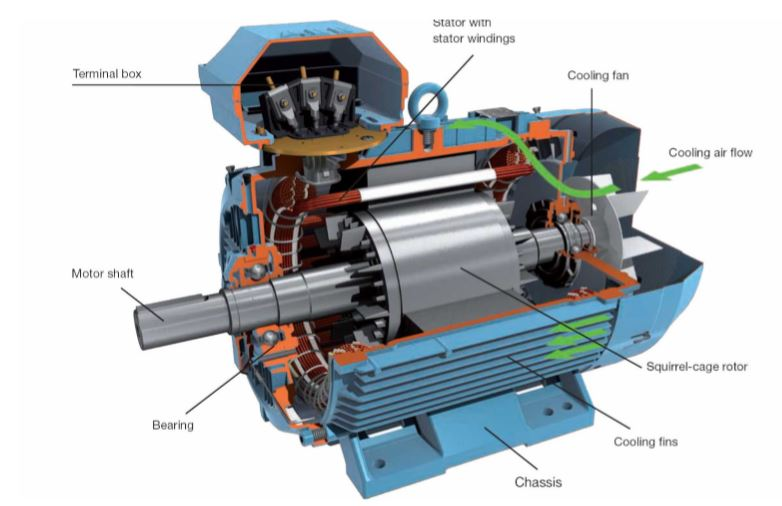
\includegraphics[width=0.75\textwidth]{./ReportImages/ValeoMotorStructure.jpg} 
    \caption{\ac{EM} Motor (Source : https://www.valeoservice.in/en-in/newsroom/basic-understanding-automotive-electric-motors)}
    \label{fig:Valeo Motor Structure}
\end{figure}

The 3 motor topologies manufactured by Valeo are displayed in Fig. \ref{fig:EM Magnet Topologies}:
\begin{enumerate}[nosep]
    \item Single V Magnet - Consists of a single V magnet shown in Fig. \ref{fig:V1 Magnet}.
    \item Double V Magnet - Consists of double V magnets shown in Fig. \ref{fig:V2 Magnet}.
    \item Nabla Magnet - Consists of a single V Magnet and a delta magnet shown in Fig. \ref{fig:Nabla Magnet}.
\end{enumerate}

\begin{figure}[H]
    \centering
    \begin{subfigure}{0.32\textwidth}
        \centering
        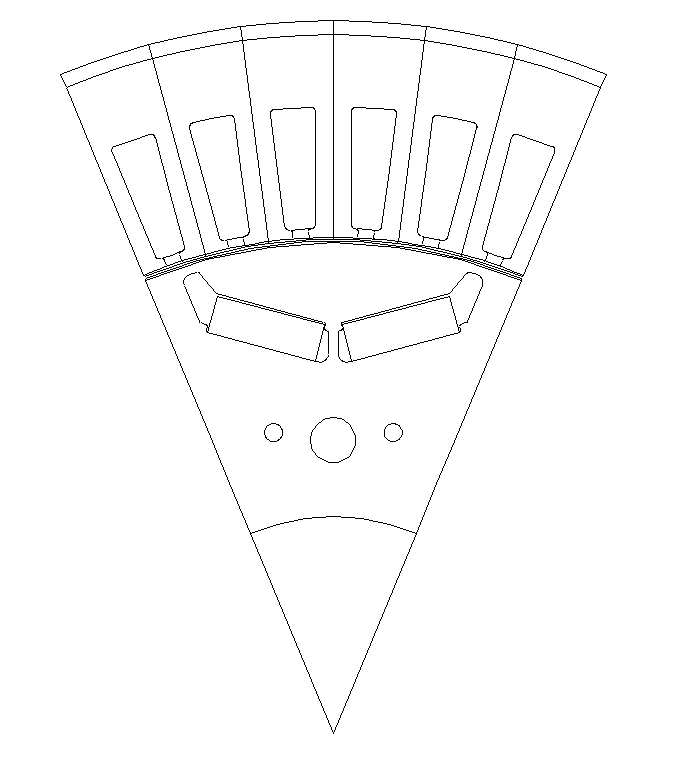
\includegraphics[width=\textwidth]{./ReportImages/1V_Magnet.png}
        \caption{Single V Magnet}
        \label{fig:V1 Magnet}
    \end{subfigure}\hfill
    \begin{subfigure}{0.32\textwidth}
        \centering
        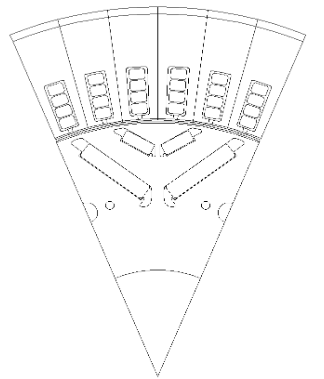
\includegraphics[width=\textwidth]{./ReportImages/2V_Magnet.png}
        \caption{Double V Magnet}
        \label{fig:V2 Magnet}
    \end{subfigure}\hfill
    \begin{subfigure}{0.32\textwidth}
        \centering
        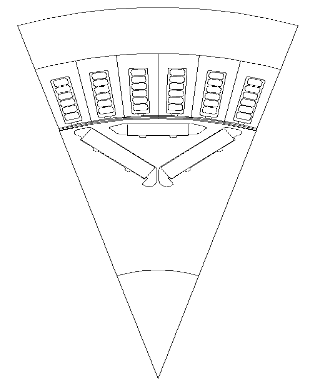
\includegraphics[width=\textwidth]{./ReportImages/Nabla_Magnet.png}
        \caption{Nabla Magnet}
        \label{fig:Nabla Magnet}
    \end{subfigure}
    \caption{\ac{EM} Magnet Topologies (Source : Valeo)}
    \label{fig:EM Magnet Topologies}
\end{figure}

Fig. \ref{fig:Torque Curve} and Fig. \ref{fig:Efficiency Grid} give a glimpse of the \ac{EM}'s \ac{KPI}s to be predicted.
\begin{figure}[H]
    \centering
    \begin{minipage}[b]{0.44\textwidth}
        \centering
        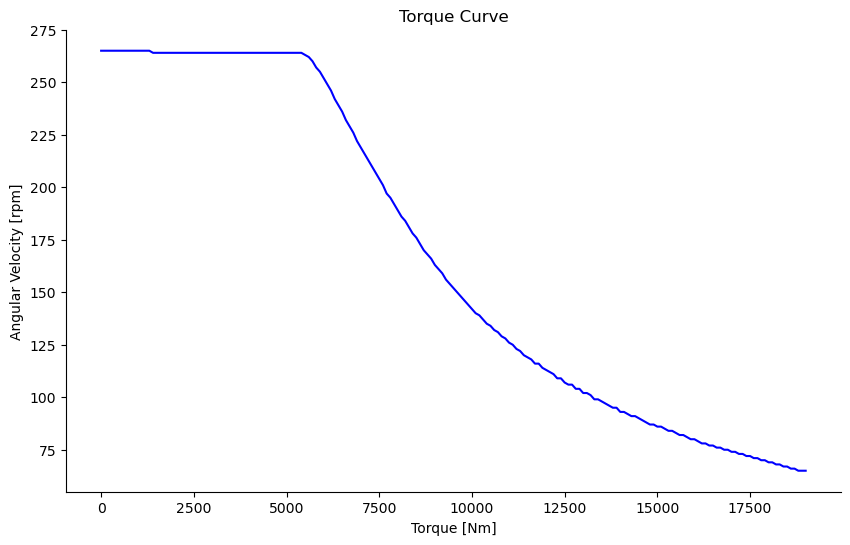
\includegraphics[width=\textwidth]{./ReportImages/TorqueCurve.png}
        \caption{Torque Curve} % Center the caption here
        \label{fig:Torque Curve}
    \end{minipage}
    \hfill
    \begin{minipage}[b]{0.54\textwidth}
        \centering
        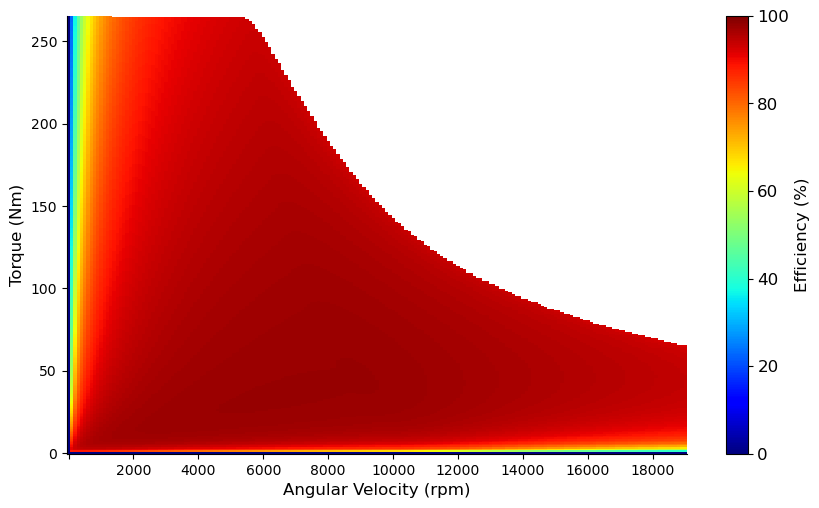
\includegraphics[width=\textwidth]{./ReportImages/EfficiencyGrid.png}
        \caption{Efficiency Grid}
        \label{fig:Efficiency Grid}
    \end{minipage}
\end{figure}
Figures Fig. \ref{fig:Torque Curve} and Fig. \ref{fig:Efficiency Grid} give a visualization of the Torque curve and the Efficiency Grid of a \ac{EM} design variant 
across angular velocities ranging from 0-19100 rpm and for positive torque values.
The angular velocities are represented as rotations per minute(rpm) and the torque as Newton meter(Nm).\\
One can observe the relation between the Torque curve and the Efficiency grid clearly from the images.
The relationship is that the Efficiency envelope is of the same shape as the Torque curve. 
The values within the Efficiency envelope can be identified with differing contour shades whose level of shading is shown to the right.\\

This master thesis explores a way to do light-weight surrogate modelling of the current process as is highlighted in Fig. \ref{fig:EM Design Flowchart} by 
exploiting data-driven deep neural networks to approximate the \ac{KPI}s derived from \ac{FEA} simulations.
Complete replacement of \ac{FEA} simulations with deep learning models is not feasible however I can exploit the use of deep neural networks 
trained on \ac{FEA} simulated data to reduce the computation burden of running these simulations repeatedly in the future.\\

Fig. \ref{fig:EM Design Flowchart} gives an outlook of both the current approach and the proposed approach to generate the \ac{KPI}s.
I discuss each component of the flowchart below :
\begin{enumerate}
    \item \textbf{\ac{EM} designs parameterized} \\
    The design of each of the \ac{EM} variants described parametrically for its geometric, physical and simulation features are regarded as the input.
    The inputs here are in its numerical equivalent format.
    \item \textbf{Current Approach}\\
    Approach followed currently by Valeo.
    \begin{enumerate}
        \item \textbf{Matlab Script 1} \\
        First a Matlab script creates a design mesh of the \ac{EM} from the parametric description of the \ac{EM}'s geometric and physical features.
        \item \textbf{\ac{FEA} simulator} \\
        Then, multiple \ac{FEA} simulations which are by nature \ac{PDE} are carried out in this \ac{EM} mesh. The \ac{FEA} solver then 
        generates the byproducts associated with the magnetic flux of the \ac{EM}.
        \item \textbf{Matlab Script 2} \\
        The outputs from the \ac{FEA} simulations are then post processed and the intermediary outputs which are matrices of values in matlab compatible format are 
        fed to the next stage.
        \item \textbf{Motor Builder} \\
        Another round of post processing is done on the magnetic flux products to generate the Power and Torque associated with the \ac{EM} design.
        Motor builder settings such as length of the motor, maximum rotation speed as well as electrical settings for instance input voltage and current are varied to 
        generate the \ac{KPI}s. The Motor Builder also is a GUI that provides visualization of the \ac{KPI} plots to the designer.
    \end{enumerate}
    \item \textbf{Proposed Approach}\\
    Approach I undertake as surrogate modelling.
    \begin{enumerate}
        \item \textbf{Data Preprocessing} \\
        The input features are preprocessed and converted into its tabular representation such that it is suitable to be fed into the Neural Network.
        For training the network, additionally the targets are taken from the \textbf{Matlab Script 2} which also serves as the ground truth represented as a dotted line.
        \item \textbf{Neural Network} \\
        I have used \ac{MLP} as the deep learning model which is made up of fully feedforward connected layers. For training, also the targets are considered to minimize 
        the loss of the predictions to be generated. However for inference, only the inputs are used to generate its approximated targets.
        \item \textbf{Data Postprocessing} \\
        The predictions generated by the neural network is post processed to be similar to the targets obtained after final postprocessing in the 
        \textbf{Motor Builder} in terms of dimensions and is plotted.
    \end{enumerate}    
    \item \textbf{KPI Plots} \\
    The targets which are vectors of numerical values are displayed graphically.
\end{enumerate}

\begin{figure}[H]
    \centering
    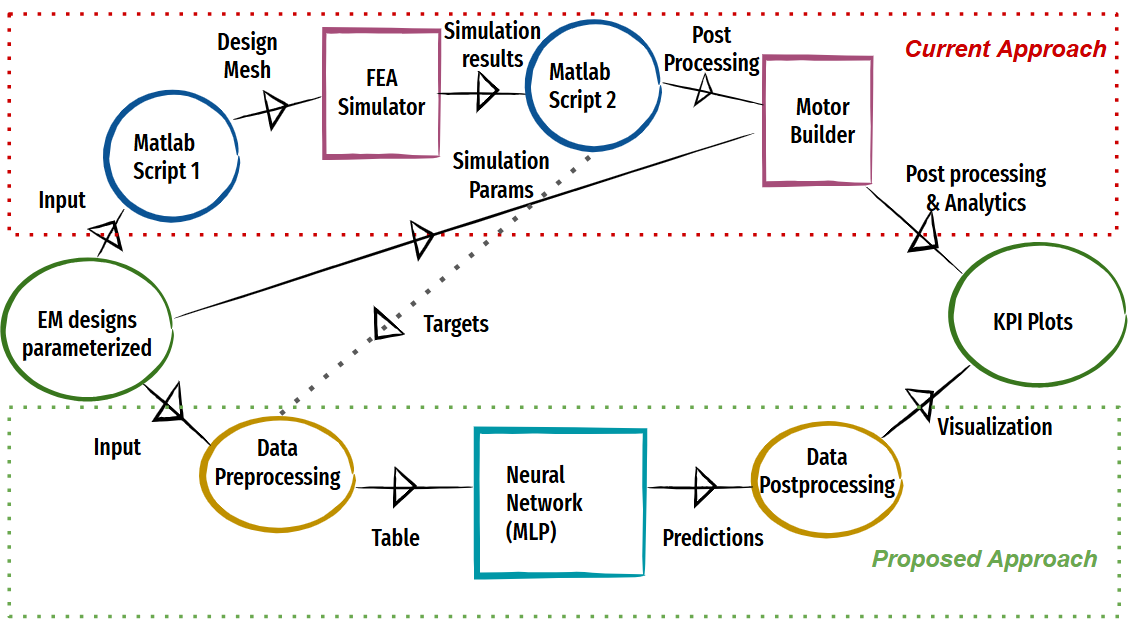
\includegraphics[width=1\textwidth]{./ReportImages/EM_design_flowchart_v2.png} 
    \caption{\ac{EM} Design Flowchart}
    \label{fig:EM Design Flowchart}
\end{figure}

\section{Objective}\label{sec:Objective}
The objective of the work is to verify whether surrogate modelling to replace \ac{FEA} simulations is feasible.
Our task is a supervised learning task to predict 2 KPIs namely the Torque curve and the Efficiency grid which are vectors of numerical values 	 
from the parametric description of topology invariant \ac{EM} and \ac{FEA} simulated \ac{KPI}s as ground truth. 
The Torque curve is a vector of torque values across certain angular velocity ranges which can be visualized as a 2\ac{D} plot whereas the Efficiency grid is a matrix of 
efficiency values of all combinations of torque ranges $\times$ angular velocities ranges and can be visualized as 3\ac{D} heatmap of contour plots. 
Both the \ac{KPI}s are continuous values which makes the task a regression problem. 
The remaining \ac{KPI}s such as Costs, Vibration losses, Torque ripple among others can be calculated from these 2 \ac{KPI}s for instance the losses 
are inversely proportional to the Efficiency values.

\section{Motivation}\label{sec:Motivation}
Our motivation to undertake this thesis is to lay the ground work for the problem's inverse formulation of generating \ac{EM} designs in the future. To my knowledge, 
there has been no work yet on Generative AI in the domain of \ac{EM} designs. The future research goal would be to condition the generative model on the predicted 
\ac{KPI}s to be able to self-generate the most efficient \ac{EM} designs. From an application standpoint, it would be beneficial for Automaker companies to refer the 
generated \ac{EM} designs to be able to suggest the most appropriate \ac{EM}s for automobiles as per customer requirements on say the horsepower of the car before manufacturing them. 
Companies could then evaluate the \ac{KPI}s of the synthetically generated \ac{EM} designs and judge on its usefulness. 

\section{Problem Statement}\label{sec:Problem Statement}

Given the Data $\mathcal{X}  = [x_1, x_2, ..., x_{n}]^T \in \mathbb{R}^{n}$, where $n$ is the number of parameters of the \ac{EM} designs. 
The targets can be referred as, Torque curve as $\mathcal{Y}_1 = [y_1, y_2, ..., y_{h}]^T \in \mathbb{R}^{h}$ where $h$ is the number of participating angular velocities and
Efficiency map as $\mathcal{Y}_2 \in \mathbb{R}^{w \times h}$ representing a grid of efficiency values defining the operating range of the \ac{EM}, where $w$ denotes 
different torque levels and $h$ the angular velocities. Each element $\mathcal{Y}_2(i,j)$ represents the efficiency at torque $i$ and angular velocity $j$.
The aim is to approximate the targets by training a \ac{MLP} model $\mathcal{M}$ to learn the mapping between $\mathcal{X}$ and $\mathcal{Y}_1$, $\mathcal{Y}_2$.

\section{Research Question}\label{sec:Research Question}

The Research Questions I aim to address are presented as follows :
 
\begin{enumerate}[nosep]
    \item \textbf{Is it feasible to predict the targets as a multi regression problem with a single model?}\\
    Since I have 2 targets of continuous values to predict, the task becomes a multi regression problem. The model architectures in Section \ref{sec:MLP Model} 
    shines light on how I go about it.
    \item \textbf{Is it possible to model an array of integer values to be predicted as a regression problem?}\\
    The Torque Curve typically harbours integers values albeit the task is in essence a regression problem which primarily works with floating point values. 
    Section \ref{sec:MLP Model} discuss how I tackle this challenge. 
    \item \textbf{How to handle varying dimensions within a target for model training?}\\
    The dimensions of the Efficiency grid differ across \ac{EM} variants. However the targets which has to be supplied to the model needs to be of a fixed size.
    I discuss in Section \ref{subsec:Deep Dive into 3D KPI} how I mitigate this problem.
    \item \textbf{How to accommodate predictions of targets of varying ranges with a single model?}\\
    The ranges among the 1st and 2nd target vary significantly and is yet another challenge I overcome in Section \ref{sec:Loss for 3D KPI}.
    \item \textbf{With a single model, how to predict 2 targets where the dimensionality of a target is dependent on the other?}\\
    Given the observation that the efficiency envelope is controlled explicitly by the torque curve. In Section \ref{sec:Post Processing}, I discuss howw to tackle this scenario.
    There has been literature on modelling wherein the values of a target are dependent on the values of another target. However, my situation is tricky in the sense 
    that instead of the values the dimensionality of the Efficiency grid is dependent on the values of the Torque curve.
\end{enumerate}

\section{Thesis Structure}\label{sec:Thesis Structure}

Over the course of the thesis I shall refer the Torque curve as Torque \ac{KPI} and the Efficiency grid as Efficiency \ac{KPI} respectively.
The remainder of the thesis is organized to follow sections namely Literature Review, Dataset, Modelling and Evaluation, Experiments and Results, Graph Modelling, Conclusion, 
Bibliography and Appendix.
In Literature Review section I review the works that has already been carried out in this domain. 
In the Dataset section a detailed insight on how the data is structured is elaborated.
In the Modelling and Evaluation section, I introduce the network architectures and loss regularization techniques used to tackle the problem.
The outcomes of the work are presented in Experiments and Results chapter in addition to other findings I unearth.
Graph Modelling section is an empirical study which I conduct outlines the background of \ac{GNN}s primarily Heterogeneous \ac{GNN}s and defines its concepts. I also attempt to 
present a workflow on how to use \ac{GNN}s for my task.
Conclusion chapter summarizes the thesis briefly and would also give a glimpse into possible areas of improvement. 
Bibliography section lists out the articles cited for this thesis. 
Lastly I share all supplementary information in the Appendix section.

\chapter{Literature Review} 

In this chapter, I attempt to review literature of works carried out in Surrogate Modelling \ac{FEA} simulations of \ac{EM} designs. In addition I have also tried to include 
writers perspectives and approaches taken across multiple stages of modelling ranging from data preprocessing to evaluation.

\section{Surrogate Modelling}\label{sec:Surrogate Modelling}

\subsection{Convolutional Neural Networks Vs Multi Layer Perceptron}\label{subsec:LR CNN Vs MLP}

There has been extensive research in modeling the \ac{EM} with \ac{CNN} based on the images of the motor cross-section. Reproducing images is not the most wisest 
approach as can be inferred from Ref. \cite{DFIG-2023} where the author presents numerous scenarios of generated images not being upto mark. These scenarios include 
difficulty to render the background accurately by only focussing on one subject, compression quality not being good enough, inability to focus on details and make 
images realistic among many other discrepancies. The research largely encompasses evaluation of image generation of faces which could be concluded that deepfakes generated were quite easy to 
distinguish from real ones.\\

Furthermore, researchers of Ref. \cite{EM CNN-2024} also presents their approach on handling surrogate modelling of topology invariant Interior 
Permanent Magnets motors to predict its Torque characteristics.
Generally the topology differs based on the count of the magnets, this is evident from the Figures in \ref{fig:EM Magnet Topologies}.
The writers claim to have used the cross-sectional images of motor designs in addition to the magnetic flux distribution of the Stator as input to the
inputs to train the \ac{CNN}. The auxiliary input is supplemented by \ac{FEA} simulations which is enriched with the nature and placement of 
the magnets in the Rotor. Although, the \ac{FEA} is used yet the product here is generated quicker and thus does not add on largely to its overhead on time complexity. 
They also claim to have improved the generalization performance of \ac{CNN}s with this strategy. In addition they suggest such domain knowledge modelling decisions 
can also be beneficial for both parameter and topology optimization of \ac{EM} as well as for prediction of its other \ac{KPI}s.\\

However, by generating the parameters of the motor one can be rest assured of more precise results. Hence the need to focus on the inputs as they are with their 
parametric description. Vivek \textit{et al.} in Ref. \cite{VAE-MT-2021} also highlights that predicting \ac{KPI}s with tabular data is significantly more efficient than 
using the images because the latter could result in less accurate designs due to the need of high resolution images in addition to its overall computation cost 
required for training. \\
Their work involves the use of a Variational Autoencoder to predict the \ac{KPI}s with an \ac{MLP} as well as sampling the latent space to 
generate new \ac{EM} designs.
Their experiments conclude that \ac{MLP}s trained on the parametric description can better infer targets such as Induced Voltage and harmonic distortion 
that are linearly dependent to the designs when compared to cogging torque which is not.
To learn the non linear functions, they also experimented with \ac{CNN}s which could infer all targets just as well as it inherently takes 
into account the pixel spatiality from motor designs as RGB images. In addition they built a hybrid model to utilize the image and parametric 
description but have comparable reported performance with that of \ac{CNN}s.
They also suggest a slight decline in accuracy for a linearly dependent target for the \ac{CNN} model as image resolution constrained the precision of the inputs.\\
Additionally, in Ref. \cite{EM SM-2023}, the authors compare and evaluate the performance of surrogate modelling Surface Permanent Magnet's parametric and image based designs.

\subsection{Machine Learning Approaches}\label{subsec:LR Machine Learning Approaches}
The authors of Ref. \cite{EM 2DFMP-2022} presents a method to predict 2\ac{D} flux maps of an Interior \ac{PMSM} motor using classical machine learning ensemble 
regression models. Therefore, for each coefficients of the 2\ac{D} flux maps, a separate regression model is trained which are then ensembled to make target predictions. 
Although there are classical Machine Learning models which handle multi regression, they do not perform very well with higher dimensions as opposed to deep neural 
networks. The writer also points out that these models fare better than deep neural networks when it comes to data required and training time.\\

Similar to my usecase for modelling \ac{EM} of cars, the writers of Ref. \cite{ETA-V-2020} experiments to compute the efficiency map of the automobile Toyota Prius. 
The methodology used is to observe Magnetic field flux density to predict how it evolves over time for different operating points of the map.\\
The paper Ref. \cite{HMLO-2021} also examines a study of how a machine learning observer can augment the performance of torque estimation of 
induction motors trained with deep neural networks. The motivation behind using the observer is made by domain aware knowledge that the torque estimated depends on 
the stator's magnetic flux. The authors claim to have made this possible by incorporating the information of speed, voltage and current into the network to realize 
the \ac{EM}'s torque. They also indicate that physics modelling of the network enabled them to develop light-weight models with better accuracy.\\

\subsection{Hybrid Models}\label{subsec:LR Hybrid Models}
The researchers of Ref. \cite{SM EMT-2020} state that the use of domain knowledge improved the accuracy of surrogate modelling \ac{EM} by creating a hybrid of both 
physics and data driven based models. In addition, it presents a workflow for surrogate modelling the air gap torque from \ac{FEA} simulated data and compares 
and contrasts the computationally efficiency with regards to both approaches. \\

Similarly, Yusuke \textit{et al.} in Ref. \cite{PANN-MT-2021} and Ref. \cite{PANN-MOO-2021} also claim that a physics assisted neural network significantly improved the accuracy 
performance when predicting the cogging torque of Permanent Magnet Synchronous Motors. Their experiments suggest that approximating the cogging torque with a 
linear subdomain model which serves as an additional input to the neural network when making the final prediction. With this methodology, they also disclose that a 
significant less data than estimated would suffice.

\subsection{Transfer Learning}\label{subsec:LR Transfer Learning}
Works by Arbaaz \textit{et al.} in Ref. \cite{EM TL-2020} explores methodologies to extend an already model to predict efficiency maps for a topology it was untrained for 
by exploiting the concept of transfer learning. The writers claim to get this accomplished by mixture of greedy pretraining and then overall finetuning the model.
They do so by freezing the pretrained network which they identify as common knowledge so that gradient flow is disabled and substitute the other 
layers of the pretrained model with new layers which is essential for the new task.\\
In addition to a topology change, this paper also explore transfer learning for different label than the pretrained model given that the labels are similar in nature 
to each other. This eventually assist the model to generalize better and conserve the time it would have spend training from scratch by knowledge reusing. 
Finetuning is a also a boon when the dataset for the new topologies are limited in existence.\\


\section{EM design generation}\label{sec:LR EM design generation}
Evolutionary algorithms such as genetic algorithms are traditionally used as multi objective optimization algorithms to generate the designs by iteratively
updating the design parameters whereas the \ac{FEA} simulations evaluate the performance of each design. 
The optimization algorithms are itself incredibly time consuming because fitness evaluation will need to be performed multiple times with \ac{FEA}.
In addition a larger number of iterations of these algorithms is necessary to evaluate each design candidate in order to explore the entire design space.
I intend to surrogate model the \ac{FEA} simulations which serves as the baseline to eliminate the role of evolutionary algorithms as well for generating designs as 
was also discussed in Section \ref{sec:Research Question}. The latter could potentially be a future work to be carried out since the time complexity associated with the 
Genetic Algorithms may discourage users to wait until convergence and rather persuade them to be satisfied with a suboptimal design.\\

Marius \textit{et al.} in Ref. \cite{VAE-MT-2021} undertake works on optimizing \ac{EM} design generation by compressing its parametric description 
across multiple topologies into a latent space using a Variational Autoencoder thereafter from which new \ac{EM} designs can be sampled.\\
Bucher \textit{et al.} in Ref. \cite{GDEM-2023} proposed a deep conditional generative design workflow to generate complete parametric 
description of Engineering Structures by taking as input the partially defined design and its performance attributes generated by \ac{FEA} software. 
The workflow comprises of a conditional variational autoencoder as proof of concept by learning a joint probability distribution between the parametric description and 
its performance attributes. \\
This would be a useful read when there is a plan to extend the current work with its inverse formulation. 
The authors also justify the usage of parametric description of the designs to be flexible for different model configurations and datasets. 
Furthermore, the writers claim that their approach as opposed to evolutionary algorithms have multiple benefits such as complete control over 
the sample space of generated designs, expressive designs, reduced computational costs and model transferability among others.

\section{Data Preprocessing Techniques}\label{sec:LR Data Preprocessing Techniques}
The authors of Ref. \cite{VAE-MT-2021} discloses the solutions taken to address the problem wherein unique parameters of 1 topology are absent in another topology.
They mitigate this concern with 2 approaches. Firstly, they default the missing values with an arbitrary fixed constant 0s this inturn pushes the model to learn a 
nonsensical value for irrelevant features. However they also note that this shortcut results in wasting model capacity making the learning unnecessarily more difficult.
Therefore, they have also used a second approach termed as Masked Learning Process wherein only features relevant for the motor topology are 
considered for modelling loss reconstruction of the model.

\section{Evaluation Techniques}\label{sec:LR Evaluation Techniques}
Arbaaz \textit{et al.} in Ref. \cite{DL-ETA-2019} attempts to generate the efficiency map by first generating its Flux linkage maps and the Torque curve 
thus accounting for geometric and operating point variations. Two interesting points are made in this paper:\\
First, since the number of excitation points vary across designs a model suitable for handling variable input sequence length is needed which implies that the values 
within the torque curve which are the excitation points are predicted. This further results in conserving training time when predicting a fixed sized grid.
They also use confusion matrix for efficiency threshold so designer can filter out efficiencies in the operating range one is most eager to find out.\\
Secondly, for efficiencies being predicted outside the excitation points, the authors propose to provide an uncertainty measure to quantify confidence level using 
Monte Carlo dropout. Reason being the error rate in the efficiency grid is maximum at the envelope of the curve. This factor gives the end user 
the flexibility to choose to generate the \ac{KPI}s with the \ac{FEA} simulations or the surrogate model.\\

Studies in Ref. \cite{EM-PM-2020} presents an interesting take on evaluating the performance of \ac{EM} with electrical engineering inspired benchmarks.
They highlight the inadequacy of evaluations generated by classical Machine Learning approaches such as \ac{MSE}, R2 Score and Symmetric Mean Absolute Percentage Error.
The argument is that these metrics favor the static area in the \ac{KPI}s which are relatively easier to predict.\\
Meanwhile the dynamic areas in the \ac{KPI}s is not projected as much having less dominance with respect to coverage area. They experimented this finding with 
Induction Motors to generate its Torque Vs Speed Predictions. The dynamic parts they considered were typically the regions in the curve before saturation is achieved. 
In such cases the Machine Learning metrics could give an over optimistic score when compared to Electrical Engineering designed metrics.\\

Researchers in Ref. \cite{DL-MF-2019} also discusses approaches to judge the accuracy with a physics-aware metric for estimating 
magnetic field of low frequency electromagnetic devices. The do so by quantifying the uncertainty of the predictions by adding a probabilistic component to the weights 
of the neurons in the network architecture. The technique they employed is known as  Monte Carlo dropout with which they generate uncertainty maps. 
The distribution of the predictions they thus generate more closely approximate that of the same generated by \ac{FEA} simulations as the accuracy improves.\\
Interestingly they also discuss the possibility of modelling the usecase with Graph Convolutional Networks instead of \ac{CNN}s.
They suggest that rather than images, graphs are better suited as they can handle unstructured design mesh which is typically fed into the \ac{FEA} simulator 
as is shown in the Fig. \ref{fig:EM Design Flowchart}. However, in my case study I aim to use \ac{GNN} on the parameteric description of the \ac{EM}. \\

The writers of Ref. \cite{ETA-LA-2020} emphasize the importance of having a very low error rate for the Efficiency Maps by \ac{FEA} simulations as the drive range of a 
vehicle's efficiency is determined with this \ac{KPI}. The Efficiency \ac{KPI}s generated by the \ac{FEA} simulations are obtained from torque, copper loss iron loss 
and mechanical loss.They study methods to further improve the accuracy of \ac{FEA} simulations of Interior Permanent Magnets by modelling the effect 
of losses such as minor hysteresis loss, stray loss, AC loss and manufacturing degradations at different operating points into these simulations.\\

\chapter{Dataset} 

Valeo has shared 1481 Excel Workbook files for each variant of three-phase interior \ac{PMSM} \ac{EM} with 8 poles and 48 slots. 
Around 89 parameters which comprises of the geometric, physical and simulation properties of the motor are chosen among the 196 parameters depending on its overall variability and significance.
This was a design decision I had made based on my understanding of the data.\\
Moreover, I detail out the structure of the dataset files in Appendix \ref{subsec:File structure}.
Fig. \ref{fig:Full Motor} shows the geometry of a whole Double V motor which can be sliced into 8 identical parts owing to the \ac{EM} design's rotational symmetry.
\begin{figure}[H]
    \centering
    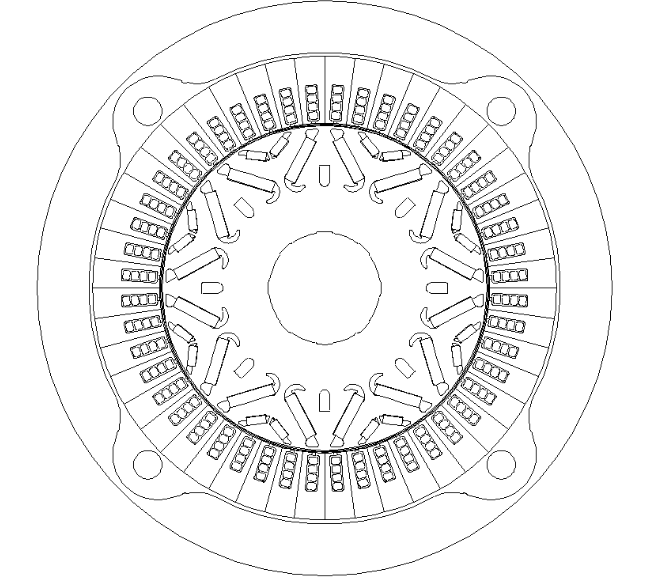
\includegraphics[width=0.4\textwidth]{./ReportImages/FullMotorv2.png} 
    \caption{Complete \ac{EM} Geometry (Source : Valeo)}
    \label{fig:Full Motor}
\end{figure}

I have also included a hand drawn sketch from my understanding of how the geometry of 1/8th cross-section of the same motor looks like in Fig. \ref{fig:1/8 Motor Crossection}.
This particularly comes in handy when creating the graph representation of the motor in Section \ref{subsec:EM Heterogeneous Graph Construction}.
From the sketch, it can be made out that the \ac{EM} very largely is comprised of the Rotor and the Stator separated by the air gap in between through the magnetic flux flows.
The Rotor hosts the permanent magnets which when rotated generates the magnetic field. These magnets sits on top of free shaped air pockets in the design. 
The free shape of these air pockets are described geometrically by oblongs which draws the shape geometrically.
The Stator comprises of the Stator poles which are 6 in number here. There are 4 slot windings for each stator slot in the tooth shoe, the slots are where the stator windings made 
up of copper sit at. The Stator yoke separates each tooth shoe from the outer radius of the \ac{EM}.

\begin{figure}[H]
    \centering
    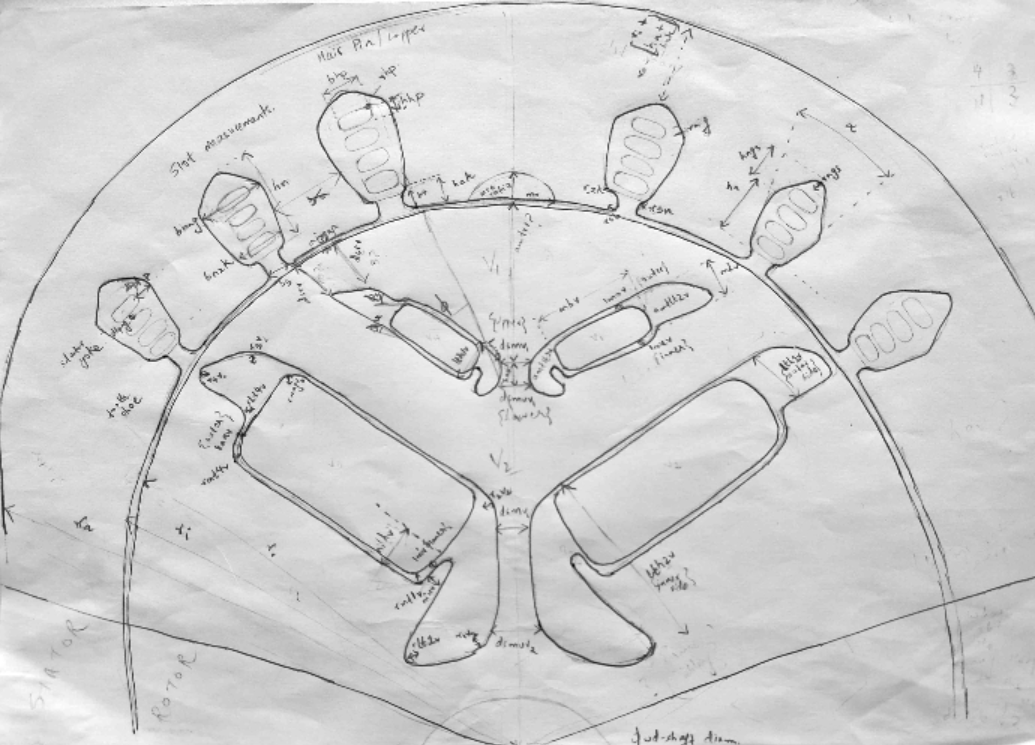
\includegraphics[width=1\textwidth]{./ReportImages/EMCrosssectionFiltered.png} 
    \caption{1/8th cross-section of \ac{EM}}
    \label{fig:1/8 Motor Crossection}
\end{figure}

\section{Data Preprocessing}\label{sec:Data Preprocessing for MLP}
For modelling the \ac{MLP}, I represent the data in tabular form with the parameters corresponding to columns. 
In Appendix \ref{subsec:Data Summary Statistics}, I provide the summary statistics of the input parameters of all the \ac{EM} variants across all 3 topologies. 
However, I focus only on the Double V Magnet Topology for the data exploration of the \ac{KPI}s as well as the dataset I use throughout the thesis for training and 
evaluation due to lack of data for the remaining two topologies. \\
Nevertheless, I have made the architecture to be compatible for the 3 topologies however I cannot draw plausible inferences from the class imbalanced topologies. \\
In order to make the data compatible with the model, some level of data processing was carried out as elaborated below.

\subsection{Data Exploration of the Input Parameters}\label{subsec:Deep Dive into Input Parameters}
All parameters including the additional ones in each topology are regarded as a separate columns and therefore if a particular column is topology dependent then the 
column corresponding to the missing data of this topology are treated as 0 values. Defaulting geometrical values as 0 seems to be the most reasonable approach in comparison 
to imputing them with the mean or median values. This is because the mean or median values are not representative of the actual data and could potentially mislead the model.\\

The values are then read and stored as their floating point equivalent to ensure data precision.
Furthermore all degree columns are converted to their equivalent radian values as all trigonometric functions expects inputs to be in radian form and radian values are of
a relatively narrow scale. 
I assumed this would be relevant given the variety of shapes in the \ac{EM} design and the fact that they are 6 phase \ac{EM} variants which implies phase shifted 
sinusoidal waves.

\subsection{Data Exploration of the Torque KPI}\label{subsec:Deep Dive into 2D KPI}
Fig. \ref{fig:Standard Deviation of 2D KPI} shows the standard deviation of 10 random handpicked samples of the Torque \ac{KPI} from the entire dataset.
The x-axis represents the angular velocity of the motor ranging from 0 to 19000 rpm. Meanwhile, the y-axis represents the torque values corresponding to the 
angular velocity. For the dataset, the range of torque values are between 55 and 280 Nm. 
The mean of all samples of the dataset is displayed with an overlap of how its standard deviation is around the mean.
Furthermore, I display a twin y-axis in red showing the standard deviation of the samples with the mean.\\

The following observations can be made from analysis of the Torque \ac{KPI}:
\begin{enumerate}[nosep]
    \item \textbf{The Standard deviation is at its peak at low angular velocities}\\
    This is evident from the Standard deviation ranging up to 3 until 5000 rpm. Beyond which the standard deviation decreases drastically until 
    saturation visible with the plateauing of the curve.
    \item \textbf{The curve to an extent resembles a mirrored S shape}\\           
    This finding is critical for how I modelled the loss regularization for the Torque \ac{KPI} and will be further elaborated in Section \ref{sec:Loss for 2D KPI}.
    \item \textbf{Samples are almost similar to one another}\\
    The samples shown here are almost resembling one another in shape and nature of curve. The finer details are at the points of the curve where it makes its transitions 
    This observation is crucial and directly impacts my decision on choosing the Baseline model to be discussed in greater detail in Section \ref{sec:Results with Baseline}.
    \item \textbf{Some Samples Standard Deviation appears to follow the mean curve}\\
    These samples are among the few whose values lies on the outliers of the approximated distribution around the mean of all samples. This becomes more 
    prominent on visualizing the results of the Torque curves and comparing the \ac{RMSE} values in Sections \ref{sec:Results with Baseline}, 
    \ref{sec:Results with MLP Efficiency KPI Regularization} among others.
    \item \textbf{Samples have a smooth curve}\\           
    From the shape of the Mean curve, it can be inferred that the samples have a smooth curve with no fluctuations. This finding is also taken into consideration in the 
    modelling phase and will be discussed in Section \ref{sec:Loss Functions} how we use it in teaching the model.
\end{enumerate}

\begin{figure}[H]
    \centering
    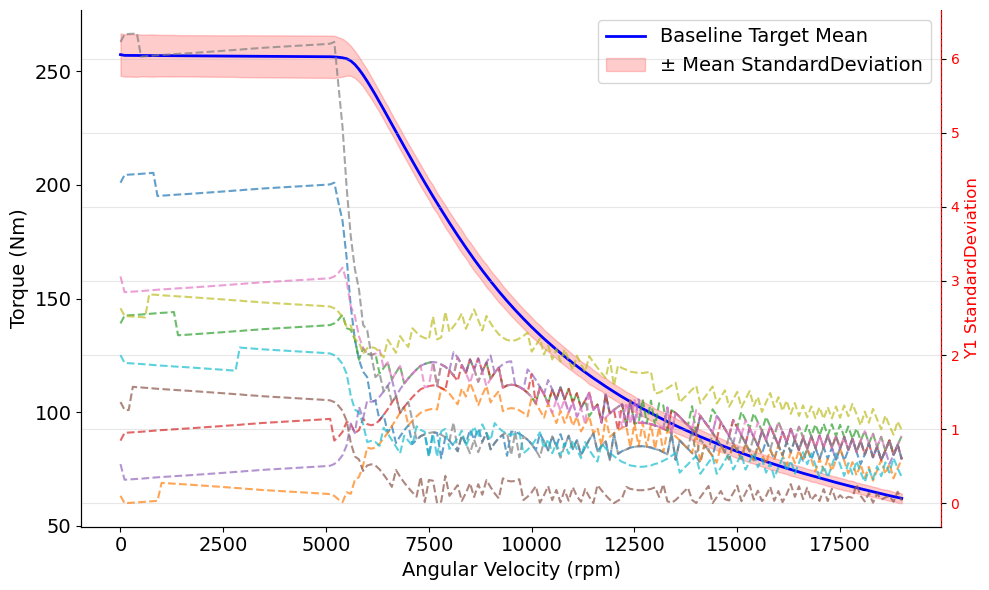
\includegraphics[width=0.6\textwidth]{./ReportImages/StandardDeviation_Baseline_y1.png} 
    \caption{Standard Deviation of Torque KPI} 
    \label{fig:Standard Deviation of 2D KPI}
\end{figure}
\subsection{Data Exploration of the Efficiency KPI}\label{subsec:Deep Dive into 3D KPI}
As the target values of the Efficiency \ac{KPI} are not provided with the same dimensions of the Torque range, I have an additional step which takes the maximum 
torque value from the Torque \ac{KPI} and slices off the Efficiency grid to only range from [- Max($\mathcal{Y}_1$), Max($\mathcal{Y}_1$)]. 
Subsequently I choose only the rows of the MM grid introduced in Table \ref{tab:Excel File Structure} which correspond to the indices of the sliced efficiency grid.
This step ensures that I grant the model the correct dimensions of the Efficiency \ac{KPI} based on its Torque \ac{KPI}.

Figures \ref{fig:Standard Deviation of Efficiency KPI(Mirrored Map)} and \ref{fig:Standard Deviation of Efficiency KPI} both illustrate the standard deviation 
of the efficiency values displayed against its angular velocity considering all samples of the dataset. The standard deviation levels are shown as a scale with colors 
darkening as the standard deviation increases.

\begin{figure}[H]
    \centering
    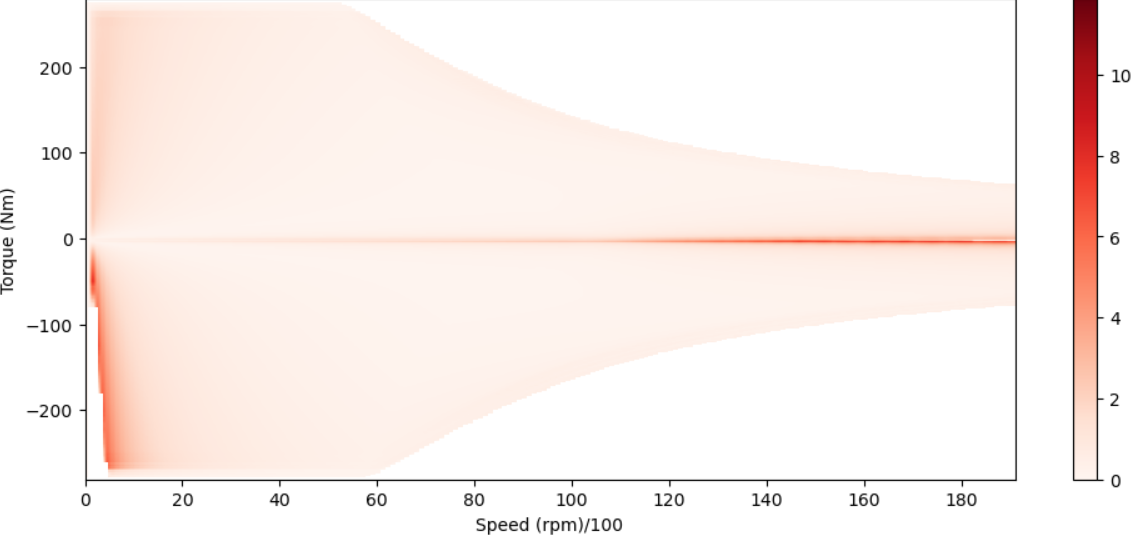
\includegraphics[width=0.7\textwidth]{./ReportImages/stddev_y2.png} 
    \caption{Standard Deviation of Mirrored Efficiency \ac{KPI}} 
    \label{fig:Standard Deviation of Efficiency KPI(Mirrored Map)}
\end{figure}

Efficiency values for negative torque values correspond to when the \ac{EM} is in generating mode and those of positive torque values to when the \ac{EM} is in 
monitoring mode.

\begin{figure}[H]
    \centering
    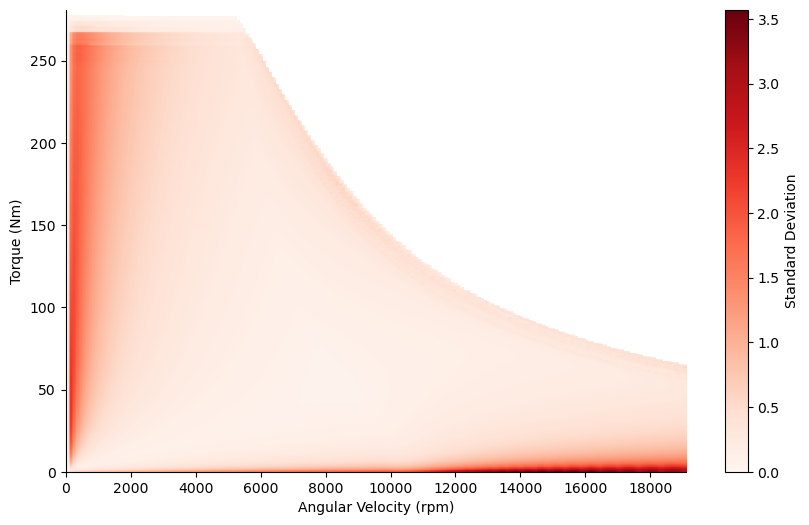
\includegraphics[width=0.6\textwidth]{./ReportImages/pos_stddev_y2.png} 
    \caption{Standard Deviation of Efficiency \ac{KPI}} 
    \label{fig:Standard Deviation of Efficiency KPI}
\end{figure}

Fig. \ref{fig:Standard Deviation of Efficiency KPI across Angular Velocity Intervals} gives us a holistic view of how the efficiency values are 
distributed across equally spaced intervals of angular velocity. The image plots the standard deviation of all the Efficiency values for all samples of the dataset 
as an error bar at certain angular velocities over equally spaced intervals of 2000 rpm.
I restrict the image to only show the Efficiency values from 2000 rpm onwards since at very low angular velocities falling in the range of 0 and 2000 rpm, the efficiency 
values vary drastically from 0\% onwards.

\begin{figure}[H]
    \centering
    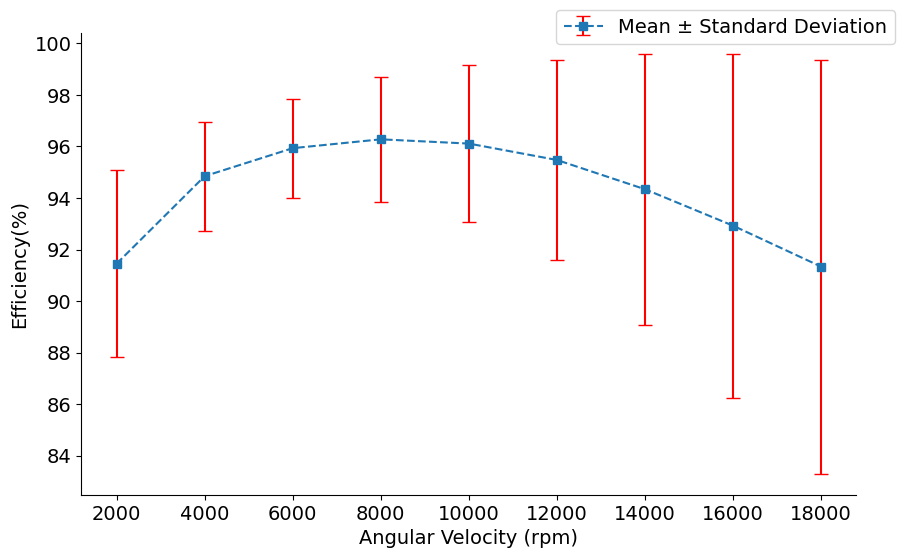
\includegraphics[width=0.6\textwidth]{./ReportImages/stddev_y2_nn_Target.png} 
    \caption{Standard Deviation of Efficiency \ac{KPI} across Angular Velocity Intervals} 
    \label{fig:Standard Deviation of Efficiency KPI across Angular Velocity Intervals}
\end{figure}

The following observations can be made from analyzing the Efficiency \ac{KPI}:
\begin{enumerate}[nosep]
    \item \textbf{Maximum deviation at low torques, extreme angular velocities}\\
    From Fig. \ref{fig:Standard Deviation of Efficiency KPI}, it can be observed that the deviation is at its peak at low torques, extreme angular velocities. 
    In Fig. \ref{fig:Standard Deviation of Efficiency KPI across Angular Velocity Intervals}, the distribution shows maximum skewness towards 
    extreme angular velocities and is relatively stable between 4000 and 6000 rpm. 
    Inn Section \ref{sec:Loss for 3D KPI}, I discuss how I integrate this finding into teaching over model. 
    \item \textbf{Efficiency values beyond the Efficiency Envelope}\\
    I also can observe that beyond the Efficiency envelope, there are no efficiency values and can be translated as blank values in the grid or \ac{NaN} values 
    in the padded Efficiency matrix, I incorporate this information in Section \ref{sec:Loss for 3D KPI}.
    \item \textbf{Considerable deviation along the Efficiency Envelope}\\
    In addition, skewness at the border of the curve within the grid can be seen in Fig. \ref{fig:Standard Deviation of Efficiency KPI}, 
    In Section \ref{sec:Post Processing} how I handle this scenario is detailed out.
    \item \textbf{Efficiency \ac{KPI} envelope is dependent on its equivalent Torque \ac{KPI} curve}\\
    As was noted already in Fig. \ref{fig:Torque Curve} and Fig. \ref{fig:Efficiency Grid}, the Efficiency \ac{KPI} envelope is completely dependent on its equivalent 
    Torque \ac{KPI} curve. The area beneath the boundary of which is looked into by the \ac{EM} manufacturers to determine the car's efficiency in the drive range.
    This is yet another finding I use in Post Processing as is further elaborated in Section \ref{sec:Post Processing}
    \item \textbf{The Efficiency grid for all samples look almost alike} \\
    I make this assumption by noting that standard deviation at its maximal is at 3. This gives us leverage to decide on choosing the Baseline model which will 
    be further discussed in Section \ref{sec:Results with Baseline}.
    \item \textbf{Efficiency values flawed in generating mode}\\
    In both monitoring and generating modes, the efficiency is almost similar albeit from Fig. \ref{fig:Standard Deviation of Efficiency KPI(Mirrored Map)}, 
    I note it is not the case for the dataset. This is evident from low angular velocity-high torque distribution area where I can see a clear distinction with \ac{NaN} values.
    Since these are \ac{FEA} simulations, it is probably an effect of a post processing step taken by the Motor builder.
    This observation made us decide on dropping the negative Efficiency \ac{KPI} and to focus on only predicting the positive Efficiency \ac{KPI}.\\
    The latter can be mirrored to replicate the efficiency when it is in generating mode if necessary.
    However over the course of this thesis, I do not do so, as it is not relevant to evaluate a duplicate again.\\
\end{enumerate}


Reading each sheet from the excel files particularly the grids take up a lot of time and compute, hence I read the files as a onetime job when creating the 
tabular data for training  and store them into pythonic objects for faster access for training.
Both the input and target values for the Torque \ac{KPI} are stored locally as csv files whereas those of the Efficiency \ac{KPI} is stored as separate csv files per 
variant considering it is in the form of a 2\ac{D} array.
The csv files are then concatenated and stored into an array conserving dimensionality by padding \ac{NaN} values to match dimensionality of the grid 
corresponding to the Torque \ac{KPI} with the largest torque value.
In my case the value is 280 computed internally from the dataset but this is subject to change as I receive more data and there is a provision to override it 
on demand. The array is then saved locally for easy access and loading during training.

Initially I had tried to set \ac{NaN} values as an incredibly high value hoping the model would consider it as a default value for prediction instead of \ac{NaN}.
However, it resulted in poor predictions as the model must have been confused and tried to increase its spread of predictions to cover this large value and so all 
true values were also predicted to be close to this dummy value.
Fortunately, I come up with a better way of handling this scenario which I elaborate in Section \ref{sec:Loss for 3D KPI}.

\section{Scaling}\label{sec:Scaling}

Scaling is a common practice done before training a neural network. 
Standard scaling is the most prevalent scaling mechanism used for normalization as it results in a Gaussian Distribution centered around the mean.
I have used the same for the input features to bring them to a common scale. \\

The Scaling is formulated mathematically as in Equation \ref{eq:Standard Scaling}
\begin{equation}
    \text{z} = \frac{x - \mu}{\sigma}
    \label{eq:Standard Scaling}
\end{equation} 
where $x$ is the Input, $\mu$ the Mean and $\sigma$ the Standard Deviation.\\
For the Input features both Mean and Standard deviation are calculated across columns. 
This is attributed to the fact I have columns with different ranges for the input since I consider each feature a column mentioned in 
Section \ref{subsec:Deep Dive into Input Parameters}.\\

I decided against scaling the targets owing to below 2 reasons :
\begin{enumerate}[nosep]
    \item They do not enter the network architecture but are only used during loss calculation.
    \item If I scale the target then I will have to scale each example from the train dataset and then average the calculated scaling parameters.
    % This in turn would mean 1 scaling parameter i.e, mean and standard deviation each for the entire dataset.
    It is not a good practice to do so as I will have lost a lot of originality in each example and is now introducing noise to new examples notably when they have a different data distribution.
    \item For the Efficiency \ac{KPI} I have loss regularization Equation \ref{eq:Y2 Maximum Efficiency Regularization} that has a constraint 
    check on the maximum range of efficiency values that can be predicted. If I had scaled the target, the constraint check would not be feasible to 
    implement as the maximum value that the constraint takes would also have to be scaled with the same scaler for comparison.\\
\end{enumerate}

During my experimentations where I initially scaled the targets, I observed then that the network required substantially less effort to learn and consequently lower learning rate and fewer epochs.
Since this comes at a tradeoff of losing precision, I continued with the original targets.
Even if I were to scale the targets, although Standard Scaling seems to be the best approach as it approximates a gaussian centered around the mean.
On the other hand, MinMax Scaler would have bound the data to be within the min and max of the data computed from the training dataset.

\section{Dataset splitting}\label{sec:Dataset splitting}
I have converted the data to be floating point tensors for better precision and collate them into a Tensor Dataset.\\
I have also partitioned the dataset to have about 50 samples for test and the remaining is used for 5 fold cross validation with 80:20 split for training and validation. 
The reason I have a separate test dataset from the validation is to ensure that there is no data leakage as I do not want to 
overfit the test dataset with the hyperparameters I choose during training. \\

Across the 5 fold training runs, 4 sets would comprise of the training set and 1 of the test set which would be different for each fold run.
Therefore weI expect to cover most grounds on training and have good monitoring on the model's performance for each fold.\\
Cross Validation also enables us to be able to monitor the network's overall stability and thus validate the model's generalization performance.\\
I have also used Data loaders to split the dataset into batches that fits into the \ac{GPU} memory.

\chapter{Modelling and Evaluation}
In this chapter, I discuss my modelling decisions of the neural network architecture, loss functions and evaluation metrics.

\section{Multi Layer Perceptron Model}\label{sec:MLP Model}

For my multi-regression problem, I use a \ac{MLP} model with input features corresponding to all the features in the tabular topology-invariant representation of the data.
The model architecture is build to predict both the Torque \ac{KPI} and Efficiency \ac{KPI}s by having 2 separate output layers for each of the \ac{KPI}s. 
Since the Torque \ac{KPI}'s targets are relatively learnable than that of the Efficiency \ac{KPI}'s targets I have experimented with fewer feed forward layers in the former than in the latter. \\
I have a hyperparameter to control the number of neurons in each hidden layer this can be tuned and is further discussed in Section \ref{tab:Hyperparameter Tunings}.\\
\ac{ReLU} layers are also added in between to serve as the activation function and produce non-linearities and consequently noise in the network. \\
Dropout layers ensure that not all neurons in each layer are used up during training to prevent the model from memorizing the data and hence overfitting.  
I have 2 hyperparameters to control the dropout rate at which I freeze the neurons when training also to be discussed in Table \ref{tab:Hyperparameter Tunings}.
I use dropout for the shared layers of the \ac{MLP} and for the layers corresponding to Efficiency \ac{KPI}.\\
Batch normalization layers are used to normalize the input from the \ac{ReLU} activations applied on it and so mitigate internal co-variate shift to the next layer and hence speed up the training process.\\
Thus both batch normalization and dropout layers stabilize the network training.\\

Fig. \ref{fig:MLP Model Architecture} gives an outline on how the \ac{MLP} Model architecture is designed and each component of the architecture is listed as follows :
\begin{enumerate}
    \item \textbf{Input} \\
    The input layer takes in all features of the tabular data which is 89 in my case as scaled tensors.
    \item \textbf{MLP Shared} \\
    The MLP Shared block is a sequential block comprising of 2 Linear Layers with the input features and neurons of each hidden layer to be a hyperparameter that needs to be tuned.
    I do not increase the number of neurons in the hidden layers within this block as it needs to be in the range of input features and output features (in this case Torque \ac{KPI}).\\
    Furthermore I have Batch Normalization layers between each linear and \ac{ReLU} activation function in addition to dropout layers.
    The dropout rate for the layers in this block is relatively higher with the intention that the model is encouraged to focus largely on learning the generality of the data.
    The 2 Linear Layers enable the network to learn a rich representation of the data during the initial feature extraction phase.
    \item \textbf{MLP Torque} \\
    This block comprises of a Linear Layer with the output feature to be the size of the Torque \ac{KPI} and a \ac{ReLU} activation function.
    I have placed a \ac{ReLU} activation function at the end of the output layer as the target values are inherently always positive values so as to exploit 
    \ac{ReLU}'s behavior of clipping negative values to 0.
    \item \textbf{MLP Efficiency} \\
    This block comprises of 3 Linear Layers with the output feature to be the size of the Efficiency \ac{KPI}.
    Here, the neurons of the hidden layers can be increased as there is not as much limitation constraining the dimensionality of the output feature which is a large grid.
    This would enable the model to be more strong and grasp the complex patterns in the data better.
    There are batch normalization, dropout and \ac{ReLU} activation functions between the 1st two Linear layers.
    The dropout rate for the layers in this block is relatively lower as there is a need to encourage the model to learn the specific nature of the grid towards the end.
    For the Last Linear layer, the dimensions of the output features corresponds to the target dimensions and a \ac{ReLU} activation is again placed after it as the target values are inherently 
    always positive values and it again encourages the model to adhere to this fact.
    \item \textbf{Torque \ac{KPI}} \\
    The number of output features correspond to the target size 191 which is infact the range of angular velocities from 0 to 19000 rpm at equal spaced intervals of 2000rpm.
    Although the targets for the Torque \ac{KPI} are an array of integer values, he float tensor and not the integer tensor are used to represent the data otherwise 
    it would become a classification problem and not a regression problem as it should be. 
    \item \textbf{Efficiency \ac{KPI}} \\
    The number of output features correspond to the target size which in my case is the shape of the padded collated array created in Section \ref{subsec:Deep Dive into 3D KPI}
\end{enumerate}

\begin{figure}[H]
    \centering
    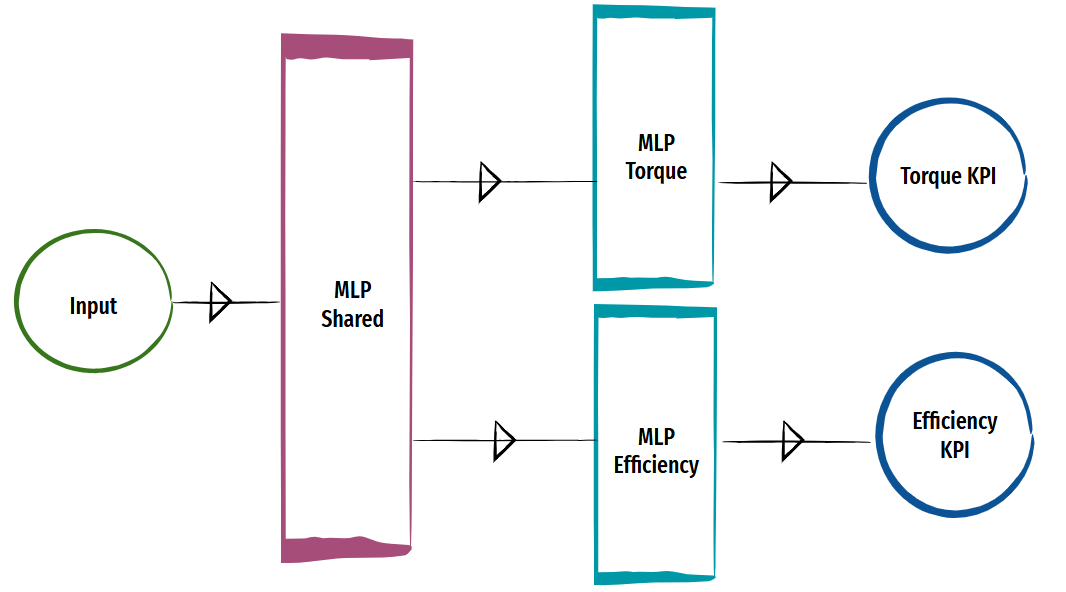
\includegraphics[width=0.8\textwidth]{./ReportImages/mlp_architecture.png} 
    \caption{\ac{MLP} Model Architecture}
    \label{fig:MLP Model Architecture}
\end{figure}

\section{Loss Functions}\label{sec:Loss Functions}
The \ac{MSE} loss is the error metric used for the problem with the intention that the squared losses penalizes the model and inturn encourage it to 
minimize the objective function even further. In addition to its contribution in exaggerating the loss by its square, \ac{MSE} also ensures that deviations are 
positive and do not confuse the model by negating the losses of opposing signs. 
\subsection{Loss for Torque KPI}\label{sec:Loss for 2D KPI}

The \ac{MSE} loss for the Torque \ac{KPI} can be formulated mathematically as shown in Equation \ref{eq:Y1 Loss}
% Mean Squared Error (\ac{MSE}) Loss for 2D KPI
\begin{equation}
    \text{$\mathcal{Y}_1$ Loss} = \frac{1}{n} \sum_{i=1}^{n} \frac{1}{h} \sum_{j=1}^{h} (y_{ij} - \hat{y}_{ij})^2,
    \label{eq:Y1 Loss}
\end{equation} 

where \(n\) is the number of \ac{EM} samples, \(h\) is the columns of the 1D Torque vector, \(y_{ij}\) and $\hat{y}_{ij}$ are the ij-th ground truth and prediction 
respectively for the torque at each operating point.\\

To encourage the model to learn the nature of the curve, I have experimented with 2 Loss Regularization techniques based on the observations from Section 
\ref{subsec:Deep Dive into 2D KPI}. 
Both of which are L2 Regularization to be in sync with the dynamics of the \ac{MSE} loss.
\begin{enumerate}
\item \textbf{Smoothening Curve Loss Regularization} \\
To smoothen out the curve for the Torque \ac{KPI}, a loss regularization factor is applied to ensure that the torque values at neighboring operating points are 
as similar as possible. This is formulated mathematically as shown in Equation \ref{eq:Y1 Smoothening Loss Regularization}.
\begin{equation}
    \text{$\mathcal{Y}_1$ Smoothening Curve Loss Regularization} = \frac{1}{n} \sum_{i=1}^{n} \frac{1}{h-1} \sum_{j=1}^{h-1}
    \begin{cases} 
        \left( \hat{y}_{ij} - \hat{y}_{i{j+1}}  \right)^2 & \text{if } |\hat{y}_{ij} - \hat{y}_{i[j+1]}| > 1, \\
        0 & \text{otherwise}.
    \end{cases}
    \label{eq:Y1 Smoothening Loss Regularization}
\end{equation}
It implies that if the difference in magnitude of consecutive values in the predicted array is greater than 1, then the loss is penalized by the square of the difference.
\item \textbf{Decreasing Curve Loss Regularization} \\
As the Torque curve closely resembles a decreasing sigmoidal curve, I use this knowledge to penalize the loss for increasing consecutive values within the prediction. 
This is intended to ensure that the torque values making up the Torque curve at each operating point is less than or equal to its prior operating point.
This is formulated mathematically as in Equation \ref{eq:Y1 Declining Loss Regularization}.
\begin{equation}
    \text{$\mathcal{Y}_1$ Declining Curve Loss Regularization} = \frac{1}{n} \sum_{i=1}^{n}\frac{1}{h-1} \sum_{j=1}^{h-1} \left(\sigma(\hat{y}_{i{j+1}} - \hat{y}_{ij})\right)^2,
    \label{eq:Y1 Declining Loss Regularization}
\end{equation} 
where $\sigma()$ is \ac{ReLU} activation function.\\
It takes into consideration the almost continuous decreasing nature of the curve as the regularization is such that a specific element in the array is less than or 
equal to its prior element.

\end{enumerate}
I have not combined the above regularizations as they do not complement each other. This is because the loss regularized by Equation 
\ref{eq:Y1 Smoothening Loss Regularization} will not necessarily be a decreasing curve.
This holds true for the regularization in Equation \ref{eq:Y1 Declining Loss Regularization} as it may not necessarily have gradual transitions in the curve.
Nevertheless, I perform ablation studies with both the regularizations and report the results in Table \ref{tab:Ablation Studies}.

\subsection{Loss for Efficiency KPI}\label{sec:Loss for 3D KPI}

The \ac{MSE} loss for the Efficiency \ac{KPI} can be translated as in Equation \ref{eq:Y2 Loss}.
\begin{equation}
\text{$\mathcal{Y}_2$ Loss} = \frac{1}{n} \sum_{i=1}^{n} \frac{1}{w} \frac{1}{h} \sum_{j=1}^{w} \sum_{k=1}^{h} \left( M_{ijk} \cdot y_{ijk}) - (M_{ijk} \cdot \hat{y}_{ijk})\right)^2,
\label{eq:Y2 Loss}
\end{equation}
\begin{equation}
    M_{ijk} = \begin{cases}
        1 & \text{if } y_{ijk} \neq \ac{NaN} \\
        0 & \text{if } y_{ijk} = \ac{NaN} 
\end{cases} ,\\
\label{eq:Mask matrix}
\end{equation}
where \(M_{ijk}\) is Mask matrix, \(w\) is the rows of 2\ac{D} vector and \(h\) the columns of 2\ac{D} vector.\\
Based on one of the observation in Section \ref{subsec:Deep Dive into 3D KPI} of the efficiency values beyond the Efficiency envelope having blank values, 
which I had also padded them to be \ac{NaN} values, I construct a binary mask matrix to ignore them in the loss calculation.
As \ac{ANN} cannot be trained to predict \ac{NaN} values, the binary mask is constructed such that values corresponding to \ac{NaN} in the target have value 0 and all other values as 1.
Mathematically, this process can be expressed as shown in Equation \ref{eq:Mask matrix} and thus ensure that the \ac{NaN} values are ignored in the loss calculation. 
The mask is then multiplied with both the target and its respective prediction. \\

I have also modelled 2 Loss Regularization techniques to encourage the model to learn the nature of the Efficiency \ac{KPI} curve.
\begin{enumerate}
\item \textbf{Maximum Efficiency Loss Regularization} \\
To ensure that the efficiency values do not exceed 100, I formulate the loss function mathematically as expressed in Equation \ref{eq:Y2 Maximum Efficiency Regularization}.
\begin{equation}
\text{$\mathcal{Y}_2$ Maximum Efficiency Regularization} = \frac{1}{n} \sum_{i=1}^{n}\frac{1}{w} \frac{1}{h} \sum_{j=1}^{w} \sum_{k=1}^{h}\left(\sigma(|\hat{y}_{ijk}| - 100)\right)^2 
\label{eq:Y2 Maximum Efficiency Regularization}
\end{equation} 

When the efficiency values of the prediction exceed 100, the overall loss is penalized by squared magnitude of the difference of the prediction from its ground truth.
\ac{ReLU} again assists to clips the difference if it is negative which is the scenario when the efficiency values are less than or equal to 100 when a violation is not warranted. \\
Needless to say the efficiency values are percentage values and can only take up values in the range of 0-100\%.
I refrain from instructing the model to not have values less than 0 since I mask \ac{NaN} values as 0 and the model will surely attempt to predict values close to 0.
Moreover, these predictions are not relevant for us as after generating all predictions I finally slice off the Efficiency grid to be of the shape of the Torque curve 
which implies that the values predicted in place of \ac{NaN} are irrelevant. This is discussed more elaborately in Section \ref{sec:Post Processing}.
Therefore, I do not see the need to needlessly punish the model for making mistakes for values I eventually do not use since pessimistic decisions could discourage the 
model from realistic learning and thus affect its focus on predicting the other values in the Efficiency grid correctly.
\item \textbf{Efficiency Grid Loss Regularization} \\
Additionally, to encourage the model to learn the nature of the Efficiency \ac{KPI} from the observations gathered in Section \ref{subsec:Deep Dive into 3D KPI}, I have 
tried to incorporate all of the following learnings into the loss function as $\mathcal{Y}_2$ Regularization techniques.
\begin{enumerate}
\item \textbf{Efficiency at Maximum Torque Loss Regularization} \\
Since I cannot regularize the loss to have the decreasing envelope of the Torque curve so I only focus on what I can effectively teach the model which 
herein is the stable portion of the Torque curve typically until Angular Velocity of 5000 rpm. This is derived from an observation I make on the shape of the Torque 
curve in Section \ref{subsec:Deep Dive into 2D KPI}.
To ensure that the shape of the Efficiency \ac{KPI} is maintained, the loss is regularized for the maximum torque value.
To do so, I have attempted to retrieve the last rows of the Efficiency \ac{KPI} and those of its target values and penalize the squared difference to have higher weight.
It is formulated mathematically as described in Equation \ref{eq:Y2_Loss_Regularization_MM_Max_Torque}.
\begin{equation}
    \text{$\mathcal{Y}_2$ Loss Regularization Max Torque} = \frac{1}{n} \sum_{i=1}^{n} \frac{1}{t_{1}} \sum_{j=-t_{1}}^{w} \frac{1}{h} \sum_{k=1}^{h} (y_{ijk} - \hat{y}_{ijk})^2,
    \label{eq:Y2_Loss_Regularization_MM_Max_Torque}
\end{equation}
where \(t_{1}\) is the threshold for initial Efficiency \ac{KPI} Envelope boundary. The number of last rows is determined by a threshold $t_{1}$.\\
\item \textbf{Efficiency at Low Angular Velocity Loss Regularization} \\
It is a known fact that at Torque 0 Nm, the corresponding efficiency values for the motor is 0\%. Consequently the efficiency values close to this torque will be low as well.
To force the model to pay more attention at lower angular velocities, the loss is regularized for the first few columns of each row of the predicted Efficiency grid 
by penalizing the squared difference with that of its target. It can be formulated mathematically as shown in Equation \ref{eq:Y2_Loss_Regularization_Low_Speed}.
\begin{equation}
    \text{$\mathcal{Y}_2$ Loss Regularization Low Angular Velocity} = \frac{1}{n} \sum_{i=1}^{n} \frac{1}{w} \sum_{j=1}^{w} \frac{1}{t_{2}} \sum_{k=1}^{t_{2}} (y_{ijk} - \hat{y}_{ijk})^2,
    \label{eq:Y2_Loss_Regularization_Low_Speed}
\end{equation}
where \(t_{2}\) is the Threshold for Low Angular Velocities. The number of first columns is determined $t_{2}$. \\
\item \textbf{Efficiency at Low Torque Loss Regularization} \\
At extreme speeds there exists a greater deviation in the efficiency values particularly towards higher speeds. This is because there are fewer efficiency values as angular velocities 
increases beyond a range since not all torque values participate.
To force the model to be more careful at low torque, the loss is regularized for the first few rows of each column of the Efficiency \ac{KPI} by penalizing the 
squared difference with that of the target. 
It can be formulated mathematically as shown in Equation \ref{eq:Y2_Loss_Regularization_Low_Torque}.
\begin{equation}
    \text{$\mathcal{Y}_2$ Loss Regularization Low Torque} = \frac{1}{n} \sum_{i=1}^{n} \frac{1}{t_{3}} \sum_{j=1}^{t_{3}} \frac{1}{h} \sum_{k=1}^{h} (y_{ijk} - \hat{y}_{ijk})^2,
    \label{eq:Y2_Loss_Regularization_Low_Torque}
\end{equation}
where \(t_{3}\) is the Threshold for Low Torque. The number of first rows is determined by $t_{3}$.\\

\end{enumerate}

The above $\mathcal{Y}_2$ Regularizations are indeed purely \ac{MSE} but with higher weights for specific regions of the Efficiency \ac{KPI}.
Consequently being L2 Regularizations it goes hand in hand with \ac{MSE} Loss calculated in Equation \ref{eq:Y2 Loss}.\\
The thresholds \(t_{1}\),\(t_{2}\) and \(t_{3}\) are tunable hyperparameters that can be optimized on observing the relevant plots of the Efficiency \ac{KPI}s visualization 
not adhering to the expected look of the Efficiency grid. The intention of including the threshold values is to give the model the flexibility to search the relevant portion of the Efficiency grid determined by the threshold 
and push the model to get those regions right by penalizing them more.\\

I aggregate all the above regularizations to form the $\mathcal{Y}_2$ Loss Regularization as described in Equation \ref{eq:Y2 Efficiency Grid Loss Regularization}.
\begin{equation}
    \begin{split}
    \text{$\mathcal{Y}_2$ Efficiency Grid Loss Regularization} = \text{$\mathcal{Y}_2$ Loss Regularization Max Torque} \\
    + \text{$\mathcal{Y}_2$ Loss Regularization Low Angular Velocity} + \text{$\mathcal{Y}_2$ Loss Regularization Low Torque}
    \end{split}
    \label{eq:Y2 Efficiency Grid Loss Regularization}
\end{equation}

\end{enumerate}

The Total Loss is calculated in Equation \ref{eq:Total Loss}.
\begin{equation}
    \begin{split}
\text{Total Loss} = \text{wt} \cdot (\text{$\mathcal{Y}_1$ Loss} + (\lambda_{\text{1y1}} \cdot \text{$\mathcal{Y}_1$ Smoothening Curve Loss Regularization}) +  (\lambda_{\text{2y1}} \cdot \\
\text{$\mathcal{Y}_1$ Declining Curve Loss Regularization })) + \text{(1-wt)} \cdot ((\text{$\mathcal{Y}_2$ Loss} + (\lambda_{\text{y21}} \cdot \\ 
\text{$\mathcal{Y}_2$ Maximum Efficiency Loss Regularization}) + (\lambda_{\text{y22}} \cdot \\
\text{$\mathcal{Y}_2$ Efficiency Grid Loss Regularization}))),
    \end{split}
    \label{eq:Total Loss}
\end{equation}
where \(\lambda_{\text{1y1}}\) is $\mathcal{Y}_1$ Smoothening Curve Loss Regularization Parameter, \(\lambda_{\text{2y1}}\) is $\mathcal{Y}_1$ Declining Curve Loss Regularization Parameter,
        \(\lambda_{\text{y21}}\) is $\mathcal{Y}_2$ Maximum Efficiency Loss Regularization Parameter, \(\lambda_{\text{y21}}\) is $\mathcal{Y}_2$ Efficiency Grid Loss Regularization Parameter, 
        \(wt\) is $\mathcal{Y}_1$ Loss Weightage, \(1-wt\) is $\mathcal{Y}_2$ Loss Weightage. \\

The Weightage parameter is utilized for the following 2 reasons:
\begin{enumerate}[nosep]
    \item  When the targets are not of the same scale. \\
    Without scaling, the losses for both targets Torque and Efficiency \ac{KPI}s being of different ranges are drastically different.
    I circumvent this by weighing up the loss of the target not performing better on validation dataset and weighing down the loss of the 
    targets by the factor of how much its value range varies.
    \item When the prediction accuracy of one \ac{KPI} is substantially more vital than the other. \\
    The task demands the same as the Efficiency \ac{KPI} is post processed to be within the shape of the Torque \ac{KPI}. \\

\end{enumerate}

Therefore, in theory have higher weightage for the Torque \ac{KPI} as its loss in performing well is costlier but because its value range is relatively higher I make the 
decisions from monitoring the predictions performance.
I reflect on these decisions based on whether the envelope of the Efficiency \ac{KPI} grid is more valuable that the efficiency values within it.\\
Ultimately I decided on prioritizing the efficiency values because to counter the Torque \ac{KPI} loss dominating the total loss, I had implemented 
quite a few regularization techniques to the Efficiency \ac{KPI} loss.\\
Furthermore, the weightage parameters for both target is designed to sum upto 1 keeping in mind improved training stability as a result of normalized weights. \\

Finally the aggregated loss is backpropagated.

\section{Optimizer}\label{sec:Optimizer}

Adam optimizer is used for optimization as it is known to be computationally efficient and requires less memory. 
It infers the gradients of the loss and how it impacts the weights and biases of each layer and thus controls learning by guiding the model to decrease the loss over the course of training. 
The optimizer acts once the loss is backpropagated across training each batch of the dataset.
The optimizer also uses the learning rate to control the step size with which the model parameters are updated.

\section{Evaluation Metrics}
The evaluation metrics regarded for the regression problem is the average of the \ac{RMSE}. 
Therefore, the model with the least prediction scores such that it is closest to 0 is the ideal score. 
Although, \ac{RMSE} is used as the metric for both evaluation and loss functions yet the loss regularizations play a strong role on the loss functions on top of \ac{RMSE}.\\
Needless to mention for the Efficiency \ac{KPI}, I have the Masking mechanism as per Equation \ref{eq:Mask matrix} which does not exists for the evaluation function of the 
same \ac{KPI} which in a way shows a pessimistic view of the model's performance. This is particularly prominent during training as I do not have visibility of the 
Efficiency envelope until its Torque \ac{KPI} values are generated. However during inference I make use of not \ac{NaN} differencing to mask out values beyond the Efficiency envelope. 

\subsection{Evaluation Metrics for Torque KPI}\label{subsec:Evaluation Metrics for 2D KPI}
The $\mathcal{Y}_1$ Score for the Torque \ac{KPI} is formulated in Equation \ref{eq:Y1 Score} :
\begin{equation}
\text{$\mathcal{Y}_1$ score} = \frac{1}{n} \sum_{i=1}^{n} \underbrace{ \sqrt{\frac{1}{h} \sum_{j=1}^{h} (y_{ij} - \hat{y}_{ij})^2}}_{\mathcal{Y}_1\ RMSE},
\label{eq:Y1 Score}
\end{equation}
where \(h\) is the columns of 1D vector and \(\mathcal{Y}_1\ \ac{RMSE}\) is \ac{RMSE} for each test sample.

\subsection{Evaluation Metrics for Efficiency KPI}\label{subsec:Evaluation Metrics for 3D KPI}
The $\mathcal{Y}_2$ score for the Efficiency \ac{KPI} is formulated in Equation \ref{eq:Y2 Score} :
\begin{equation}
    \text{$\mathcal{Y}_2$ score} = \frac{1}{n} \sum_{i=1}^{n} \underbrace{ \sqrt{\frac{1}{w} \frac{1}{h} \sum_{j=1}^{w} \sum_{k=1}^{h} (y_{ijk} - \hat{y}_{ijk})^2}}_{\mathcal{Y}_2\ RMSE},
    \label{eq:Y2 Score}
\end{equation}
where \(w\) is the rows of 2\ac{D} vector, \(h\) is columns of 2\ac{D} vector and \(\mathcal{Y}_2\ \ac{RMSE}\) is the \ac{RMSE} for each test sample.\\

The Aggregated $\mathcal{Y}$ score for \ac{KPI}s is formulated in Equation \ref{eq:Aggregated Score}.
\begin{equation}
    \text{Aggregated $\mathcal{Y}$ score} = \text{wt} \cdot (\text{$\mathcal{Y}_1$ score}) + (1-\text{wt}) \cdot (\text{$\mathcal{Y}_2$ score}),
    \label{eq:Aggregated Score}
\end{equation}
where $wt$ and  $1-wt$ are the weightage assigned to is $\mathcal{Y}_1$ score and $\mathcal{Y}_2$ score respectively. 
It is the same weightage assigned to aggregate the losses of both the \ac{KPI}s in Equation \ref{eq:Total Loss}.\\

As the value ranges for both the \ac{KPI}s are so starkly different, I give a glimpse of the corresponding percentage differences and have narrowed down scoring to 
follow the criteria as recorded in Table \ref{tab:Scoring Criteria}.
\begin{table}[H]
    \centering
    \begin{tabularx}{1\linewidth}{|X|X|X|X|X|X|X|X|X|X|}
    \hline {\bf \% Difference} & {\bf 0-5\%} & {\bf 5-10\%} & {\bf 10-15\%} & {\bf 15-20\%} & {\bf 20-25\%} & {\bf 25-30\%} & {\bf 30-35\%} & {\bf 35-40\%} & {\bf 40-100\%}\\
    \hline 
    $\mathcal{Y}_1$ Score& 0-11& 11-22 & 22-33 & 33-44 & 44-55& 55-66 & 66-77 & 77-88 & \textgreater 88\\
    $\mathcal{Y}_2$ Score& 0-5 & 5-10 & 10-15 & 15-20 & 20-25& 25-30 & 30-35 & 35-40 &\textgreater 40\\
    \hline
    \end{tabularx}
    \caption{Scoring Criteria}
    \label{tab:Scoring Criteria}
\end{table}

This is deduced from the Equations \ref{eq:Y1 Percentage Difference} and \ref{eq:Y2 Percentage Difference}.
\begin{equation}
    \text{$\mathcal{Y}_1$ Percentage Difference} = (\text{$\mathcal{Y}_1$ Score} / {(Max(\mathcal{Y}_1) - Min(\mathcal{Y}_1))})  \cdot 100
    \label{eq:Y1 Percentage Difference}
\end{equation}
\begin{equation}
    \text{$\mathcal{Y}_2$ Percentage Difference} = (\text{$\mathcal{Y}_2$ Score} / {(Max(\mathcal{Y}_2) - Min(\mathcal{Y}_2))})  \cdot 100
    \label{eq:Y2 Percentage Difference}
\end{equation}

From my observations of the dataset, the target values for Torque \ac{KPI} range between 50-280 and those of the Efficiency \ac{KPI} range between 0-100.
The scoring of the $\mathcal{Y}_2$ at inference is slightly different from that of training in the sense that for inference, I have the Torque \ac{KPI} to 
accurately slice of the envelope from the Efficiency \ac{KPI}. However, during training I do not have the Torque \ac{KPI} generated yet to slice the Efficiency \ac{KPI}.

\section{Post Processing}\label{sec:Post Processing}
The mean and standard deviation from the train-validation datasets are applied to transform the test dataset to maintain uniformity in the predictions generated.
In the case of new files not part of the segregated test dataset, I first convert it into the tabular representation the model consumes and then apply the scaling.
This is why I preserve the same scalers used during training as I not only evaluate the dedicated test dataset but also new files for clients to use on demand. 

Furthermore as I am predicting a padded matrix to ensure dimensionality sync across different Efficiency \ac{KPI}s, the grid contains values even outside the boundary 
of the Efficiency \ac{KPI}.
First I attempt to slice of the grid to ignore 0 values for all rows excluding the 1st row as per the Equation \ref{eq:Y2_Loss_Regularization_Low_Speed} in the 
hopes that the Mask constructed from equation \ref{eq:Mask matrix} would force the model to learn 0s. However it tried to approximate values close to 0 and was almost never 0.\\
Therefore, I decided to slice the shape of the Torque \ac{KPI} curve from the Efficiency \ac{KPI} by counting the number of columns a row can have based on consecutive 
values in the curve.
This brings us back to the point that it is imperative that the prediction of the Torque \ac{KPI} is close to perfect since the envelope of the Efficiency \ac{KPI} is 
inherently dependent on it.
However if in the worst case scenario where the $\mathcal{Y}_1$ and $\mathcal{Y}_2$ predictions are so starkly different that Efficiency \ac{KPI} cannot be sliced off from 
the Torque \ac{KPI} because the former is smaller than the latter then I decide not to slice the Efficiency \ac{KPI} and instead use the predictions as is. I also 
prompt the end user a warning when this scenario is encountered.

\chapter{Experiments and Results}

\section{Experiments}\label{sec:Experiments with MLP}

After optimizing over an exhaustive random search of the hyperparameter space, I present the chosen hyperparameters in Table \ref{tab:Hyperparameter Tunings} by 
monitoring the model's performance across 5 fold cross validation. I use different splits for each round of training and tune the hyperparameters on the validation set. 
The final splits are saved locally and can be used later to ensure reproducibility. 

\begin{table}[H]
    \centering
    % \begin{tabularx}{1\linewidth}{|X|X|X|X|}
    \begin{tabularx}{\linewidth}{|p{0.625\textwidth}|p{0.15\textwidth}|p{0.145\textwidth}|}
    \hline {\bf Hyperparameters} & {\bf Value} & {\bf Value Ranges}\\
    \hline 
    Learning Rate (\textit{lr}) & 0.075 & 0.025 - 0.25\\
    Dimensionality of Hidden Layers (\textit{hidden size})& 128 & 64, 128\\
    Exponential Learning Rate Scheduler Gamma (\textit{lr gamma})& 0.9 & 0.5-0.9\\
    Batch Size (\textit{batch size})& 72 & 32-72\\
    Number of Epochs (\textit{epochs})& 10 & 6-10\\
    Dropout Probability for Shared Layers (\textit{$p_{y1}$})& 0.35 & 0.4-0.2\\
    Dropout Probability for Efficiency Layers (\textit{$p_{y2}$}) & 0.2 & 0.2-0.1\\
    $\mathcal{Y}_1$ Smoothening Curve Loss Regularizer (\textit{$\lambda_{1y1}$}) & 0.5 & 0-0.75\\
    $\mathcal{Y}_1$ Decreasing Curve Loss Regularizer (\textit{$\lambda_{2y1}$})& 0.5 & 0-0.75\\
    $\mathcal{Y}_2$ Maximum Efficiency Value Regularizer (\textit{$\lambda_{y21}$})& 3 & 0-5\\
    $\mathcal{Y}_2$ Efficiency Grid Loss Regularizer (\textit{$\lambda_{y22}$}) & 5 & 0-5\\
    $\mathcal{Y}_2$ Initial Envelope Boundary Threshold (\textit{$t_{1}$})& 5 & 0-5\\
    $\mathcal{Y}_2$ Low Speed Threshold (\textit{$t_{2}$})& 20 & 0-30\\
    $\mathcal{Y}_2$ Low Torque Threshold (\textit{$t_{3}$})& 20 & 0-30\\
    Weightage of $\mathcal{Y}_1$ Loss (\textit{wt})& 0.05 & 0-1\\
    Weightage of $\mathcal{Y}_2$ Loss (\textit{1-wt})& 0.95 & 0-1\\
    \hline
    \end{tabularx}
    \caption{Hyperparameter Tuning}
    \label{tab:Hyperparameter Tunings}
\end{table}

I am using an exponential learning rate scheduler which reduces the learning rate exponentially by the \textit{lr gamma} to decay learning as training progresses across epochs.
This is to ensure that the model does not overshoot after few epochs of training.\\
I also would like to point out that the 2 outputs typically would thrive on different learning rates and might be a better approach to have separate learning rates in addition 
to separate loss functions.\\
The \textit{batch size} is limited to the capacity of the \ac{GPU} memory. I use the maximum batch size to train faster after which I hit the memory roof of the \ac{GPU}.\\
The \textit{hidden size} refers to the number of neurons in the hidden layers of the \ac{MLP} model. I have experimented with just 2 hidden sizes as I am 
constrained by the fact that the number of neurons must be between the range of input features and output features which was discussed in Section \ref{sec:MLP Model}.
In addition it has to be of the multiples of 8 as \ac{GPU}s are most optimized for the same.\\
Dropout rate during training is controlled by the parameter \textit{$p_{y1}$} for shared layers and \textit{$p_{y2}$} for layers specific to Efficiency \ac{KPI}. 
This is discussed in Section \ref{sec:MLP Model}. I am not so much concerned of the data being dropped in larger extent for the Efficiency \ac{KPI} than anticipated 
for the Torque \ac{KPI} because the latter is relatively simpler to learn and the value range larger leading to its loss dominating the total loss.\\
\textit{$\lambda_{1y1}$}, \textit{$\lambda_{2y1}$}, \textit{$\lambda_{y21}$} and \textit{$\lambda_{y22}$} parameters control the regularization weight for the 
regularization terms for the Torque \ac{KPI} and Efficiency \ac{KPI} respectively detailed in Equation \ref{eq:Total Loss}.
The thresholds \textit{$t_{1}$}, \textit{$t_{2}$} and \textit{$t_{3}$} are used to control the number of rows and/or columns to be considered for the loss
regularization terms to learn the nature of the Efficiency \ac{KPI} as discussed in Section \ref{sec:Loss for 3D KPI}.
The weightage parameter to control the direction of loss is denoted by \textit{wt} and is also discussed in Equation \ref{eq:Total Loss}.\\
I also observe that a simple architecture of the model is not a significant downside for limited data set as it seems to learn the patterns within the data 
especially since I supplement the loss regularization with more knowledge.

\subsection{Monitoring MLP with Efficiency Grid Regularization}\label{subsec:Monitoring MLP with Efficiency Grid Regularization}

We monitor the \ac{MLP} model which only uses the loss regularization parameters \textit{$\lambda_{y21}$} and \textit{$\lambda_{y22}$} and it does not consider the loss  
regularization for the Torque \ac{KPI}s whose performance I discuss in Sections \ref{sec:Ablation Studies}.\\
I have chosen a 3rd party application \texttt{Wandb}\footnote{Weights \& Biases - \url{https://wandb.ai/}} to log metrics from the training run and to monitor model 
performance across the 5 folds. Training and validation occurs 5 times on different combinations of cross validation splits independent per fold.\\

Fig. \ref{fig:Training Loss Metrics} illustrates the loss at work as training progresses across epochs. 
Figures \ref{fig:Training Loss for Torque Curve} and \ref{fig:Training Loss for Efficiency grid} provides monitoring of how the losses for both the \ac{KPI}s vary. 
As was discussed in Equation \ref{eq:Y1 Loss} and Equation \ref{eq:Y2 Loss}, both the \ac{MSE} losses 
also include their respective loss regularization terms weighted by the tunable regularization coefficients. 
Fig. \ref{fig:Aggregated Training Loss} depicts the weighted sum of the losses discussed in Equation \ref{eq:Total Loss}.
The Validations plots for losses also tells us the same tale although the Efficiency \ac{KPI} stops to learn after a certain point can be monitored in Fig. 
\ref{fig:Validation Loss Metrics}.

\begin{figure}[H]
    \centering
    \begin{subfigure}{0.32\textwidth}
        \centering
        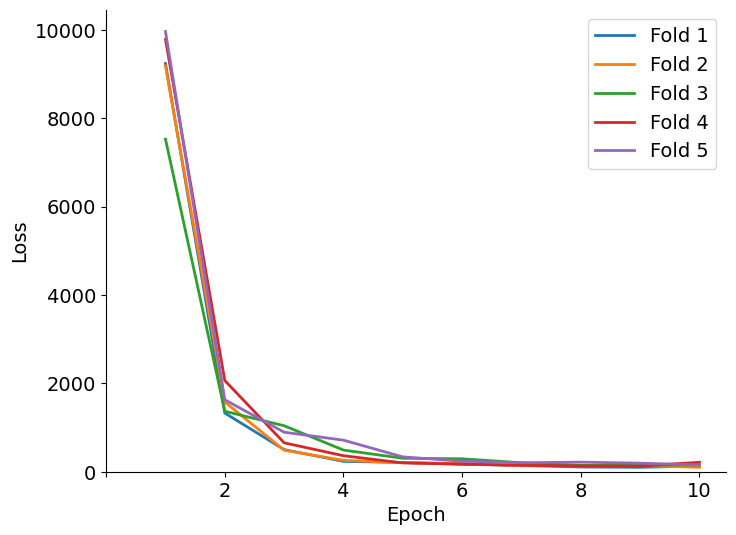
\includegraphics[width=\textwidth]{./ReportImages/train_loss.png}
        \caption{\centering Aggregated}
        \label{fig:Aggregated Training Loss}
    \end{subfigure}\hfill
    \begin{subfigure}{0.32\textwidth}
        \centering
        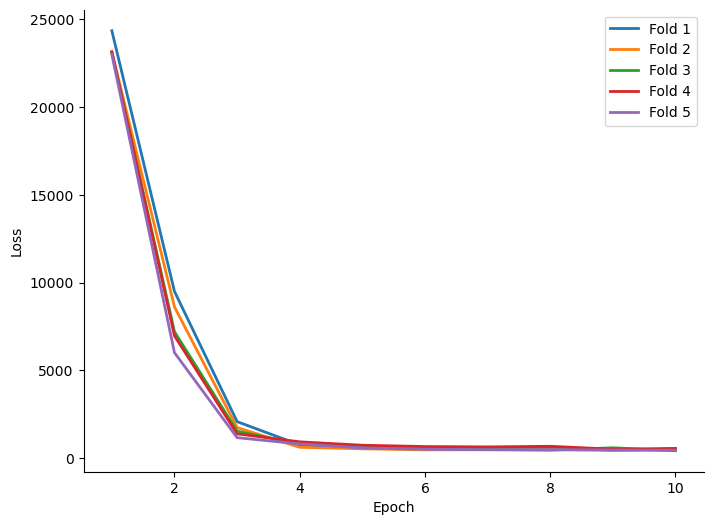
\includegraphics[width=\textwidth]{./ReportImages/train_loss_y1.png}
        \caption{\centering Torque \ac{KPI}}
        \label{fig:Training Loss for Torque Curve}
    \end{subfigure}\hfill
    \begin{subfigure}{0.32\textwidth}
        \centering
        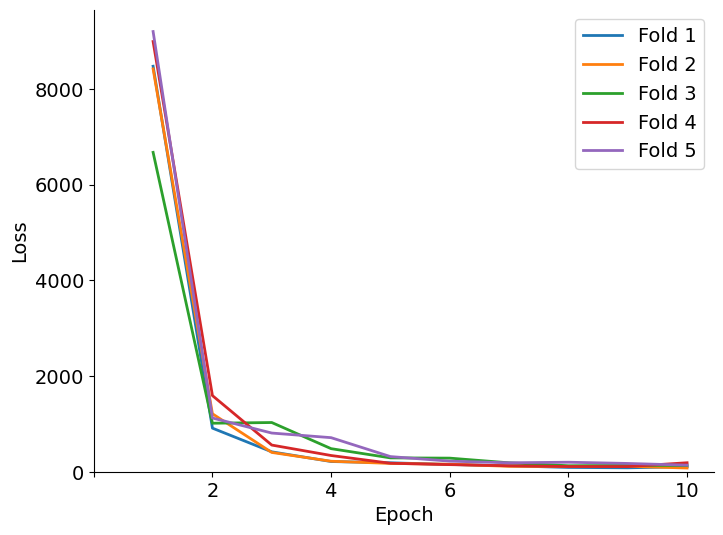
\includegraphics[width=\textwidth]{./ReportImages/train_loss_y2.png}
        \caption{\centering Efficiency \ac{KPI}}
        \label{fig:Training Loss for Efficiency grid}
    \end{subfigure}
    \caption{Training Loss Metrics}
    \label{fig:Training Loss Metrics}
\end{figure}

Fig. \ref{fig:Validation Evaluation Metrics} illustrates the evaluation metrics changing across each epoch of the validation dataset. This is important to us to know 
the model's performance on unseen data fot the 5 folds. Fig. \ref{fig:Aggregated Validation Score} shows the aggregated validation score which is again the weighted 
sum of the scores as was formulated in Equation \ref{eq:Aggregated Score} for both the \ac{KPI}s.
Meanwhile, Fig. \ref{fig:Validation Score for Torque Curve} and Fig. \ref{fig:Validation Score for Efficiency grid} logs monitoring of the evaluation metrics as per the 
Equation \ref{eq:Y1 Score} and Equation \ref{eq:Y2 Score}.
Likewise the training plots evaluation metrics are displayed in Fig. \ref{fig:Training Evaluation Metrics}.\\

The following are the observations I infer from monitoring the training and validation plots:

\begin{enumerate}[nosep]
    \item The model has converged after having run for 10 epochs with a total run time of 2 minutes where each fold took around 20s.
    \item Even though the weightage assigned to the Efficiency \ac{KPI} is significantly more in addition to loss regularization parameter, it seems to have stopped learning 
    beyond a threshold and so I hypothesize to further increase the weightage of the Efficiency \ac{KPI}.
\end{enumerate}

\begin{figure}[H]
    \centering
    \begin{subfigure}{0.32\textwidth}
        \centering
        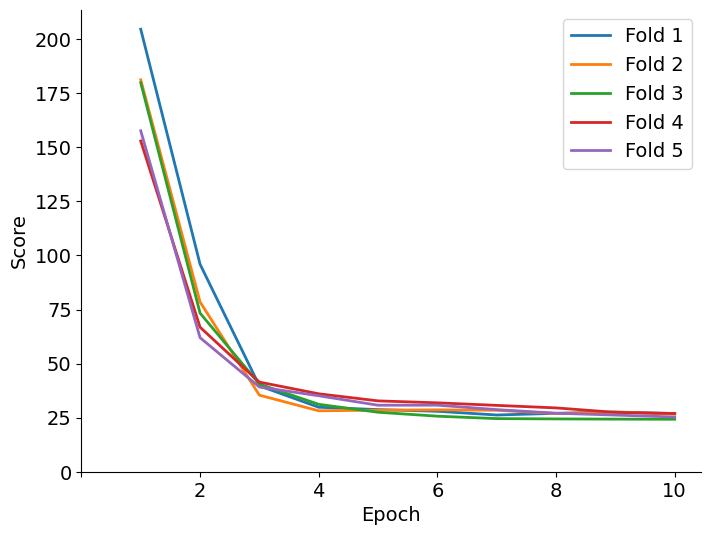
\includegraphics[width=\textwidth]{./ReportImages/val_score.png}
        \caption{\centering Aggregated}
        \label{fig:Aggregated Validation Score}
    \end{subfigure}\hfill
    \begin{subfigure}{0.32\textwidth}
        \centering
        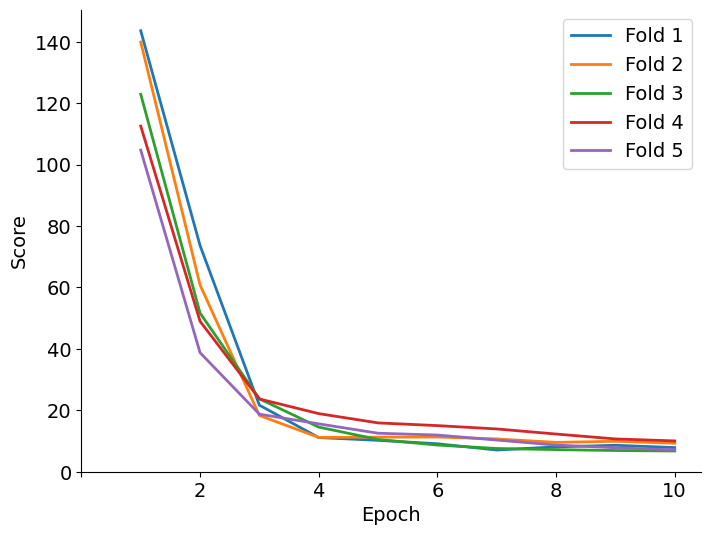
\includegraphics[width=\textwidth]{./ReportImages/val_score_y1.png}
        \caption{\centering Torque \ac{KPI}}
        \label{fig:Validation Score for Torque Curve}
    \end{subfigure}\hfill
    \begin{subfigure}{0.32\textwidth}
        \centering
        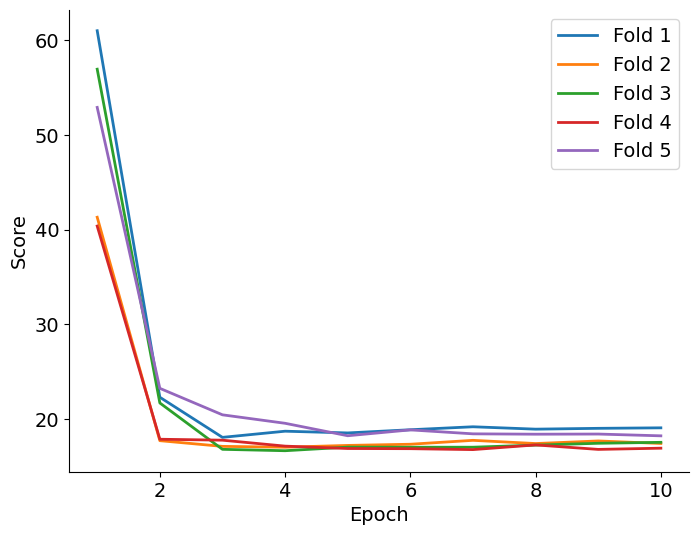
\includegraphics[width=\textwidth]{./ReportImages/val_score_y2.png}
        \caption{\centering Efficiency \ac{KPI}}
        \label{fig:Validation Score for Efficiency grid}
    \end{subfigure}
    \caption{Validation Evaluation Metrics}
    \label{fig:Validation Evaluation Metrics}
\end{figure} 

The training loss and validation evaluation plots are most important to us to be able to judge the hyperparameters to optimize. 
Therefore the other plots are moved to Appendix \ref{sec:Experimental setup} for further reflection.
I have also enabled saving the best performant fold locally so it can be loaded on demand by the client when in needs to only run inference.

\section{Results with MLP Efficiency KPI Regularization}\label{sec:Results with MLP Efficiency KPI Regularization}
The model we have used here is the \ac{MLP} model with the Efficiency \ac{KPI} loss regularization terms.
\subsection{Torque KPI Results}\label{subsec:Torque KPI Results with MLP Efficiency KPI Regularization}

\begin{figure}[H]
    \centering
    \includegraphics[width=.9\textwidth]{./ReportImages/KPI2D_predictions.png} 
    \caption{MLP Predictions for Torque \ac{KPI}} 
    \label{fig:MLP Training Results for 2D KPI(Torque)}
\end{figure}

Fig. \ref{fig:MLP Training Results for 2D KPI(Torque)} illustrates 6 samples from the test dataset for the predicted Torque values and their corresponding ground truths 
displayed against their angular velocities. The difference and percentage difference between the prediction and ground truth are also displayed on a twin y axis to 
give a rough overview of the prediction deviations from the targets. As the percentage difference formulated in Equation \ref{eq:Y1 Percentage Difference} would 
always result in positive values, they appear above the 0 line dotted separator.\\

Fig. \ref{fig:MLP RMSE Evaluation for 2D KPI(Torque)} displays the Average \ac{RMSE} and element wise \ac{RMSE} for 10 samples from the test dataset with its predictions 
from the model. 
This figure closely resembles the skeleton of the Fig. \ref{fig:Standard Deviation of 2D KPI} in terms of what is displayed in addition to the samples used. 
The only difference that can be highlighted is that the \ac{RMSE} with that of the ground truth is displayed instead of standard deviation on the twin y-axis in red.

\begin{figure}[H]
    \centering
    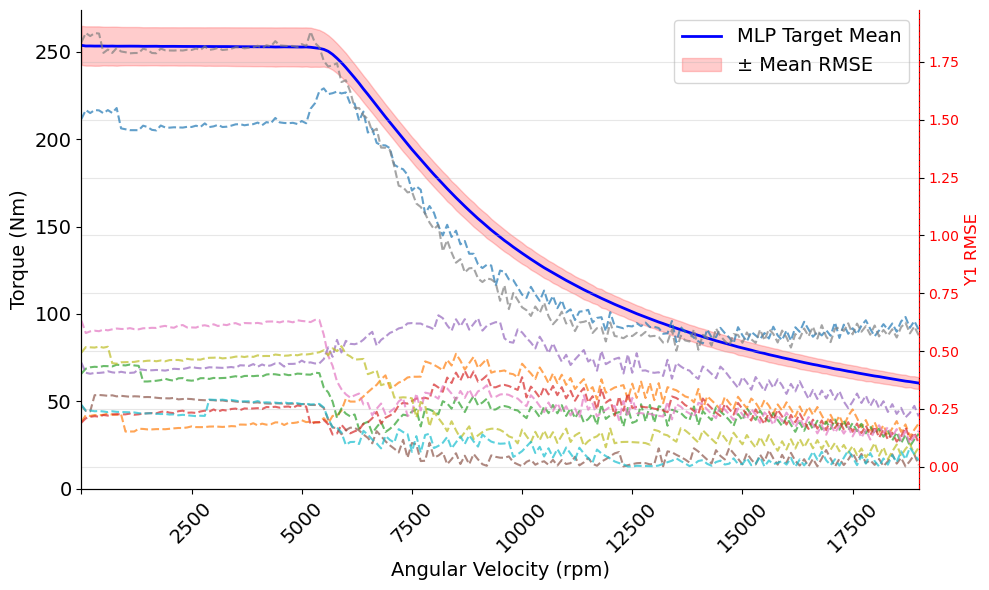
\includegraphics[width=0.6\textwidth]{./ReportImages/RMSE_MLP_y1.png} 
    \caption{\ac{MLP} \ac{RMSE} Evaluation for Torque \ac{KPI}} 
    \label{fig:MLP RMSE Evaluation for 2D KPI(Torque)}
\end{figure}

Fig. \ref{fig:Y1 Evaluation Statistics MLP} shows the score statistics of the model performance of Torque \ac{KPI} over all samples from the test dataset 
with the number of test dataset samples on the y-axis.
The $\mathcal{Y}_1$ \ac{RMSE} from Equation \ref{eq:Y1 Score} is calculated for each sample and shown as a histogram in Fig. \ref{fig:Y1 RMSE}.
In addition the $\mathcal{Y}_1$ Percentage Difference from Equation \ref{eq:Y1 Percentage Difference} is also calculated for each sample and shown as a histogram in Fig. 
\ref{fig:Y1 Evaluation Statistics MLP}. The latter is essential to be able to relate to its effect on total range of deviation due to its differing value range. 
The histogram looks the same in shape for both the figures however the finer details lies within the measure on the x-axis.

\begin{figure}[H]
    \centering
    \begin{subfigure}{0.5\textwidth}
        \centering
        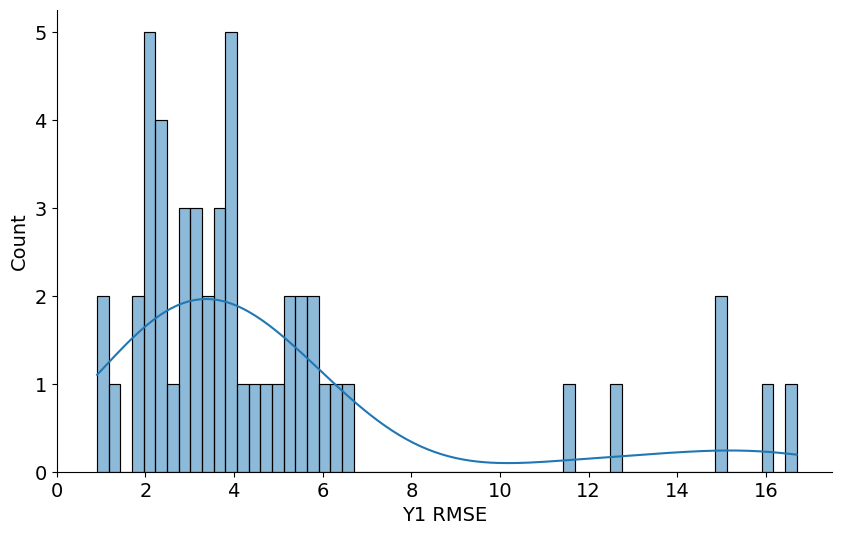
\includegraphics[width=\textwidth]{./ReportImages/score_MLP_y1.png}
        \caption{$\mathcal{Y}_1$ \ac{RMSE}}
        \label{fig:Y1 RMSE}
    \end{subfigure}\hfill
    \begin{subfigure}{0.5\textwidth}
        \centering
        \includegraphics[width=\textwidth]{./ReportImages/percentage_diff_MLP_y1.png}
        \caption{$\mathcal{Y}_1$ Percentage Difference}
        \label{fig:Y1 Percentage Difference}
    \end{subfigure}
    \caption{$\mathcal{Y}_1$ Evaluation Statistics of \ac{MLP}}
    \label{fig:Y1 Evaluation Statistics MLP}
\end{figure}

Fig. \ref{fig:MLP Training Deviation across Folds for Torque KPI} gives a good view of how the torque curve for each folds prediction represented in dotted lines deviate 
from the mean of all the folds predicted torque curve. I also take care to note that I have used only 1 sample from the test dataset for inference across all folds.\\

\begin{figure}[H]
    \centering
    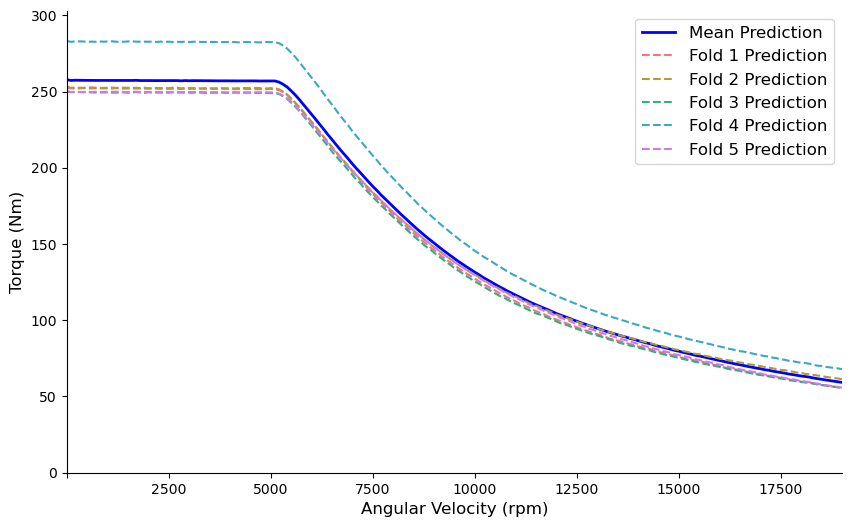
\includegraphics[width=0.6\textwidth]{./ReportImages/folds_dev_y1.png} 
    \caption{MLP Training Deviation across Folds for Torque \ac{KPI}} 
    \label{fig:MLP Training Deviation across Folds for Torque KPI}
\end{figure}

The following are the observations I infer of the Torque \ac{KPI} from the model:

\begin{enumerate}[nosep]
    \item In Fig. \ref{fig:MLP Training Results for 2D KPI(Torque)} although deviations can be seen, it can be noticed for few of the cases the predictions are such 
    that the torque values predicted have smaller values than its respective ground truths. However, most of the examples show very close correlation between prediction 
    and ground truth and percentage differences on average do not exceed 5\%. 
    \item In Fig. \ref{fig:MLP RMSE Evaluation for 2D KPI(Torque)}, the \ac{RMSE} equivalent to the $\mathcal{Y}_1$ score tells us that for 80\% of the plots shown, 
    the predictions are off by less than 5\% from the target values by cross-referencing Table \ref{tab:Scoring Criteria}. 
    Only for 2 samples a greater deviation can be noticed however these are the samples discussed in 
    \ref{subsec:Deep Dive into 2D KPI} as outliers from the mean distribution. 
    \item The predicted Torque curves closely resemble the trajectory of the target values although they fluctuate. Experimenting with the hyperparameters 
    \textit{$\lambda_{1y1}$} and \textit{$\lambda_{2y1}$} has potential to improve this anomaly. In addition, granting a higher weight \textit{wt} for $\mathcal{Y}_1$ 
    can also help in this direction.
    \item It can be deduced from Fig. \ref{fig:Y2 Evaluation Statistics MLP} that the $\mathcal{Y}_1$ scores are approximately gaussian distributed between 
    0.5-4 with outliers for 5 samples upto 7.5 thus encompassing a range of 0-4\% percentage difference with the target values as derived from the table \ref{tab:Scoring Criteria}.
    \item It can be remarked from Fig. \ref{fig:MLP Training Deviation across Folds for Efficiency KPI} that the predicted torque curves for all the folds except Fold 4 
    is as close as can be to each other. Although the torque values predicted by Fold 4 are relatively larger values, it can be observed that the shape of the curve is 
    approximated correctly in all folds. This image is a good indicator of the model's generalization capability and also sheds light to the model's stability.
    \item The Torque \ac{KPI} shows promise in learning better but it would be at the cost of overfitting the Efficiency \ac{KPI}.
    \\
\end{enumerate}

MOVE A noteworthy point is that I have left the output predictions for the Torque curve to remain as floating point values even when the target values are integers 
to preserve data precision. The client has the flexibility to turn this on/off demand. 

\subsection{Efficiency KPI Results}\label{subsec:Efficiency KPI Results with MLP Efficiency KPI Regularization}
Fig. \ref{fig:Efficiency KPI Predictions Vs Targets with MLP} shows 3 sample predictions of the Efficiency \ac{KPI} from the test dataset alongside its ground truth.
Torque is displayed against its angular velocities and all efficiency values within the envelope can be viewed as differing colors in a contour plot. 
The figures are augmented with a scale showing the efficiency values in percentage across varying levels. 

\begin{figure}[H]
    \centering
    \begin{subfigure}{1\textwidth}
        \centering
        \includegraphics[width=1\textwidth]{./ReportImages/KPI3Dprediction1.png} 
        \caption{1st Sample} 
        \label{fig:1st Sample}
    \end{subfigure}\hfill
    \begin{subfigure}{1\textwidth}
        \centering
        \includegraphics[width=1\textwidth]{./ReportImages/KPI3Dprediction2.png} 
        \caption{2nd Sample} 
        \label{fig:2nd Sample}
    \end{subfigure}\hfill
    \begin{subfigure}{1\textwidth}
        \centering
        \includegraphics[width=1\textwidth]{./ReportImages/KPI3Dprediction3.png} 
        \caption{3rd Sample} 
        \label{fig:3rd Sample}
    \end{subfigure}
    \caption{Efficiency \ac{KPI} Predictions Vs Targets with \ac{MLP}},
    \label{fig:Efficiency KPI Predictions Vs Targets with MLP}
\end{figure} 

I have also taken the liberty of displaying the error margin as the overlap difference 
of the predicted and target efficiency values for the aforementioned samples in Fig. \ref{fig:Efficiency KPI Predictions Vs Targets Vs Difference with MLP}. 
The margins of the errors can be seen as levels referring to the difference in efficiencies to the right of each subplot. The 3 subplots are the prediction, target 
and its difference respectively such that all of them are displayed side by side for easy comparison. \\
I visualize the images for the same samples in Fig. \ref{fig:Efficiency KPI Predictions Vs Targets Vs Difference with MLP} however in a smaller scale to accommodate 
a 3rd figure denoting difference overlap. Thus, the figures in \ref{fig:Efficiency KPI Predictions Vs Targets with MLP} serve to give a larger view for comparing and 
contrasting the predictions and its targets.

\begin{figure}[H]
    \centering
    \begin{subfigure}{1\textwidth}
        \centering
        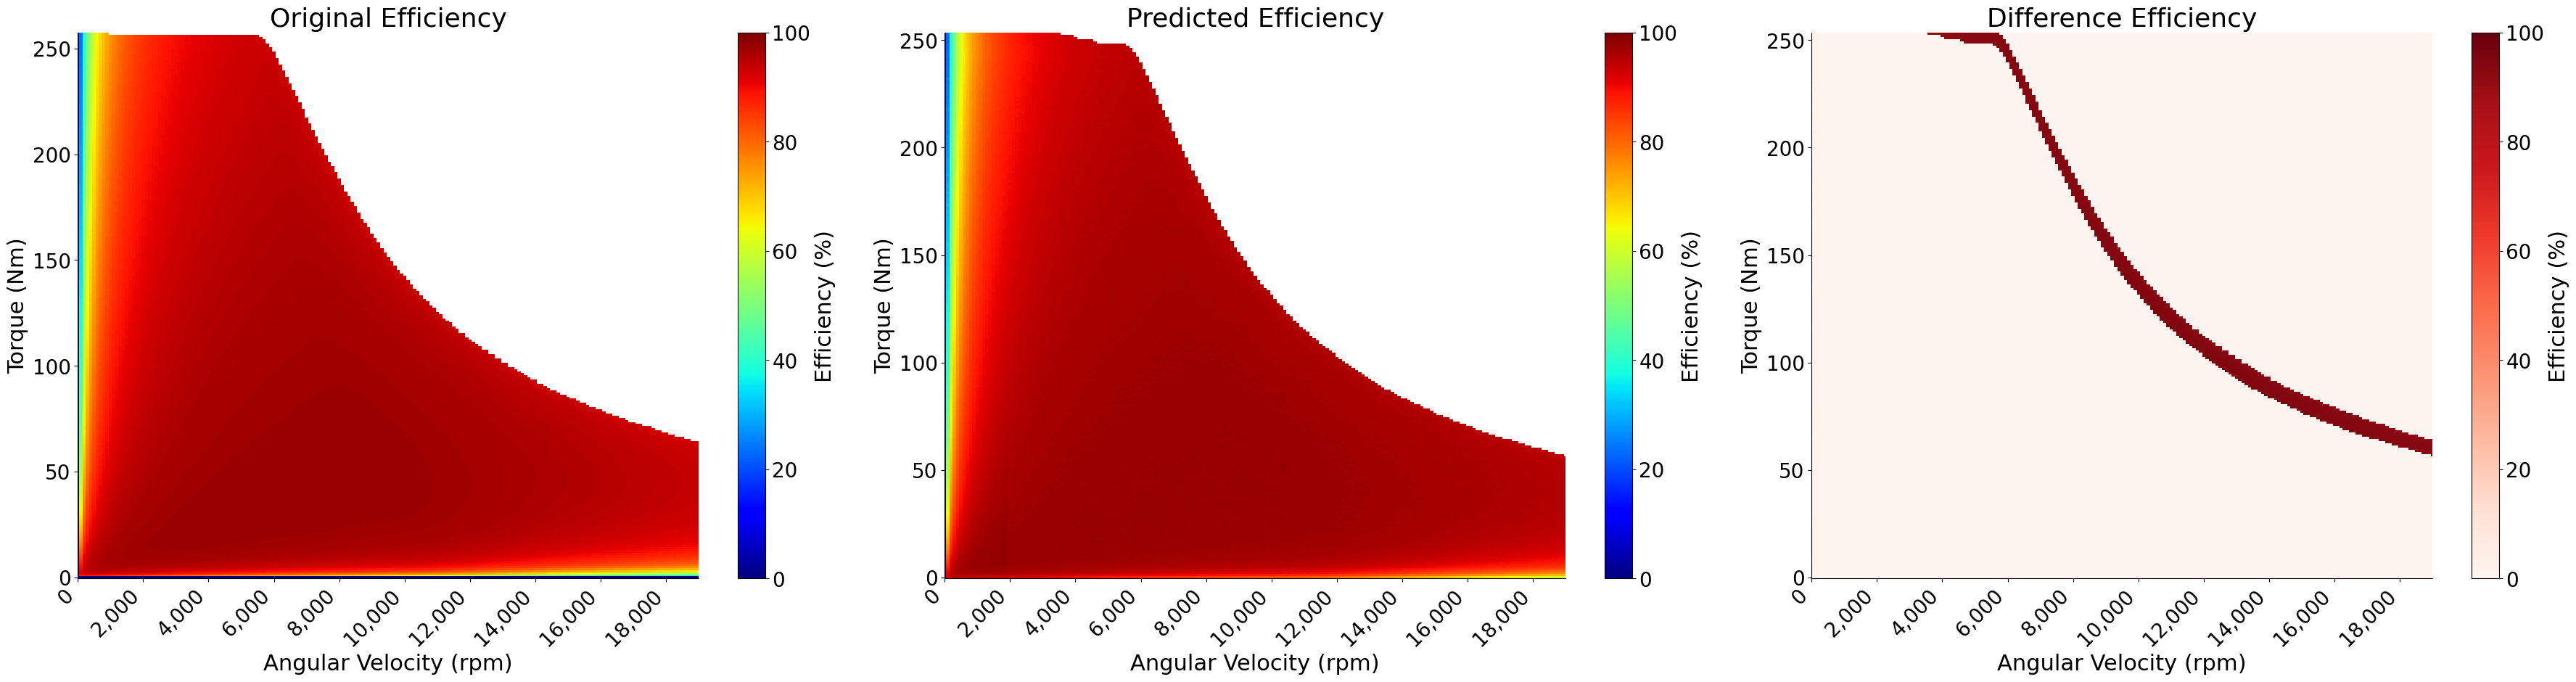
\includegraphics[width=1\textwidth]{./ReportImages/evalkpi3dprediction1.png} 
        \caption{1st Difference Sample} 
        \label{fig:1st Difference Sample}
    \end{subfigure}\hfill
    \begin{subfigure}{1\textwidth}
        \centering
        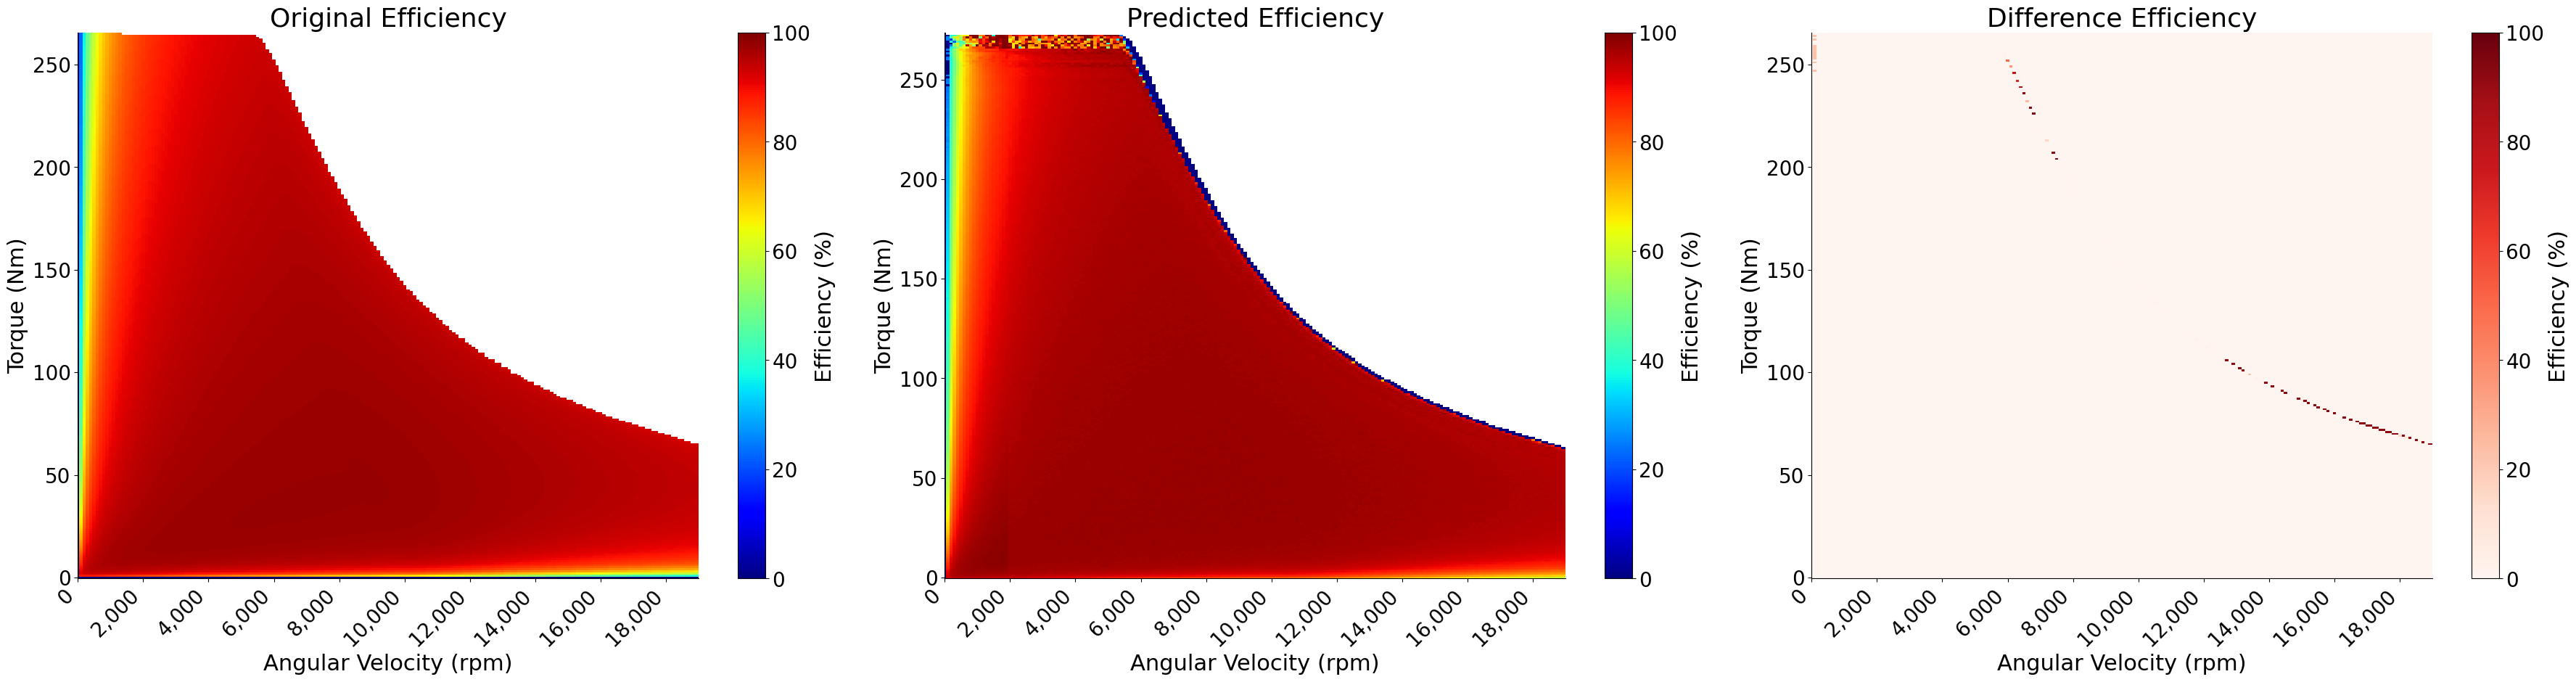
\includegraphics[width=1\textwidth]{./ReportImages/evalkpi3dprediction2.png} 
        \caption{2nd Difference Sample} 
        \label{fig:2nd Difference Sample}
    \end{subfigure}\hfill
    \begin{subfigure}{1\textwidth}
        \centering
        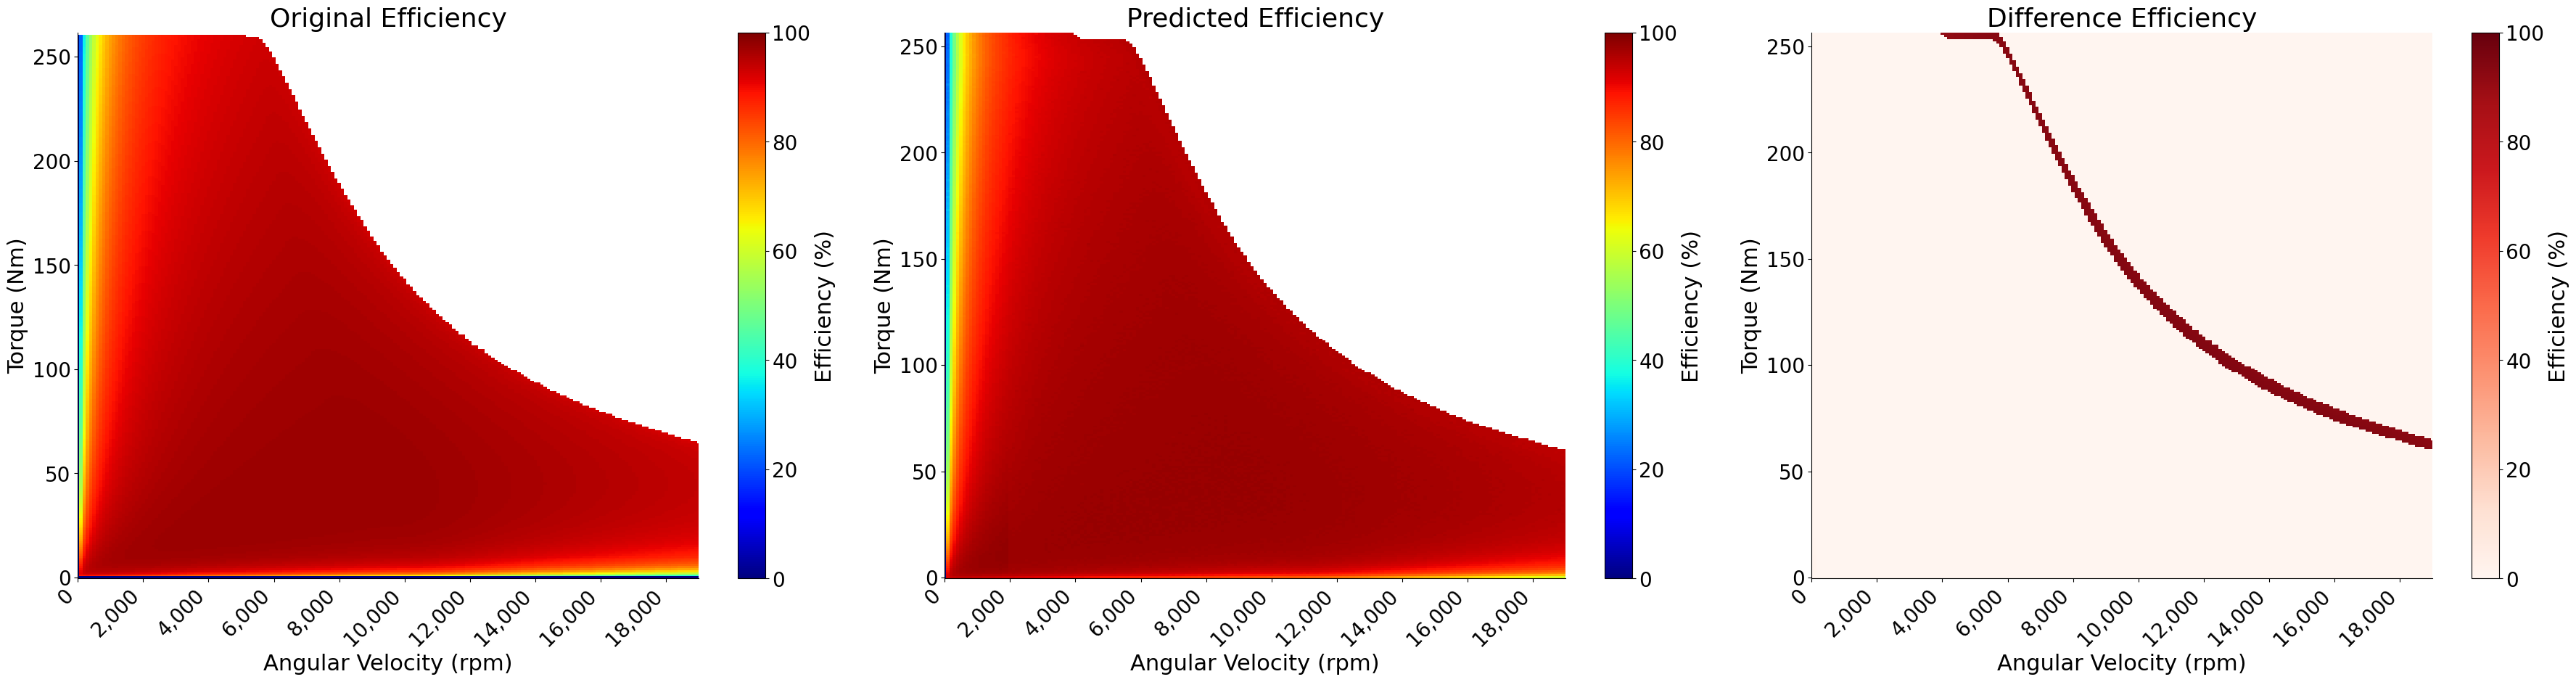
\includegraphics[width=1\textwidth]{./ReportImages/evalkpi3dprediction3.png} 
        \caption{3rd Difference Sample} 
        \label{fig:3rd Difference Sample}
    \end{subfigure}
    \caption{Efficiency \ac{KPI} Predictions Vs Targets Vs Difference with \ac{MLP}},
    \label{fig:Efficiency KPI Predictions Vs Targets Vs Difference with MLP}
\end{figure} 

Fig. \ref{fig:MLP Standard Deviation of 3D KPI(Efficiency) across Angular Velocity Intervals with MLP} depicts the standard deviation across different 
angular velocity ranges for the model's predictions as error bar plots. The structure of the image is similar to Fig. 
\ref{fig:Standard Deviation of Efficiency KPI across Angular Velocity Intervals}

\begin{figure}[H]
    \centering
    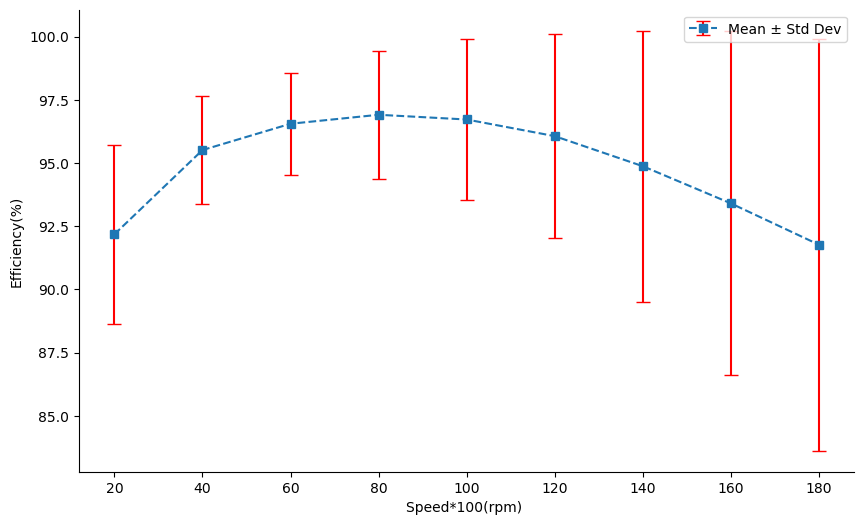
\includegraphics[width=0.6\textwidth]{./ReportImages/stddev_y2_nn_MLP.png} 
    \caption{\ac{MLP} Standard Deviation of Efficiency \ac{KPI} across Angular Velocity Intervals with \ac{MLP}} 
    \label{fig:MLP Standard Deviation of 3D KPI(Efficiency) across Angular Velocity Intervals with MLP}
\end{figure}

\begin{figure}[H]
    \centering
    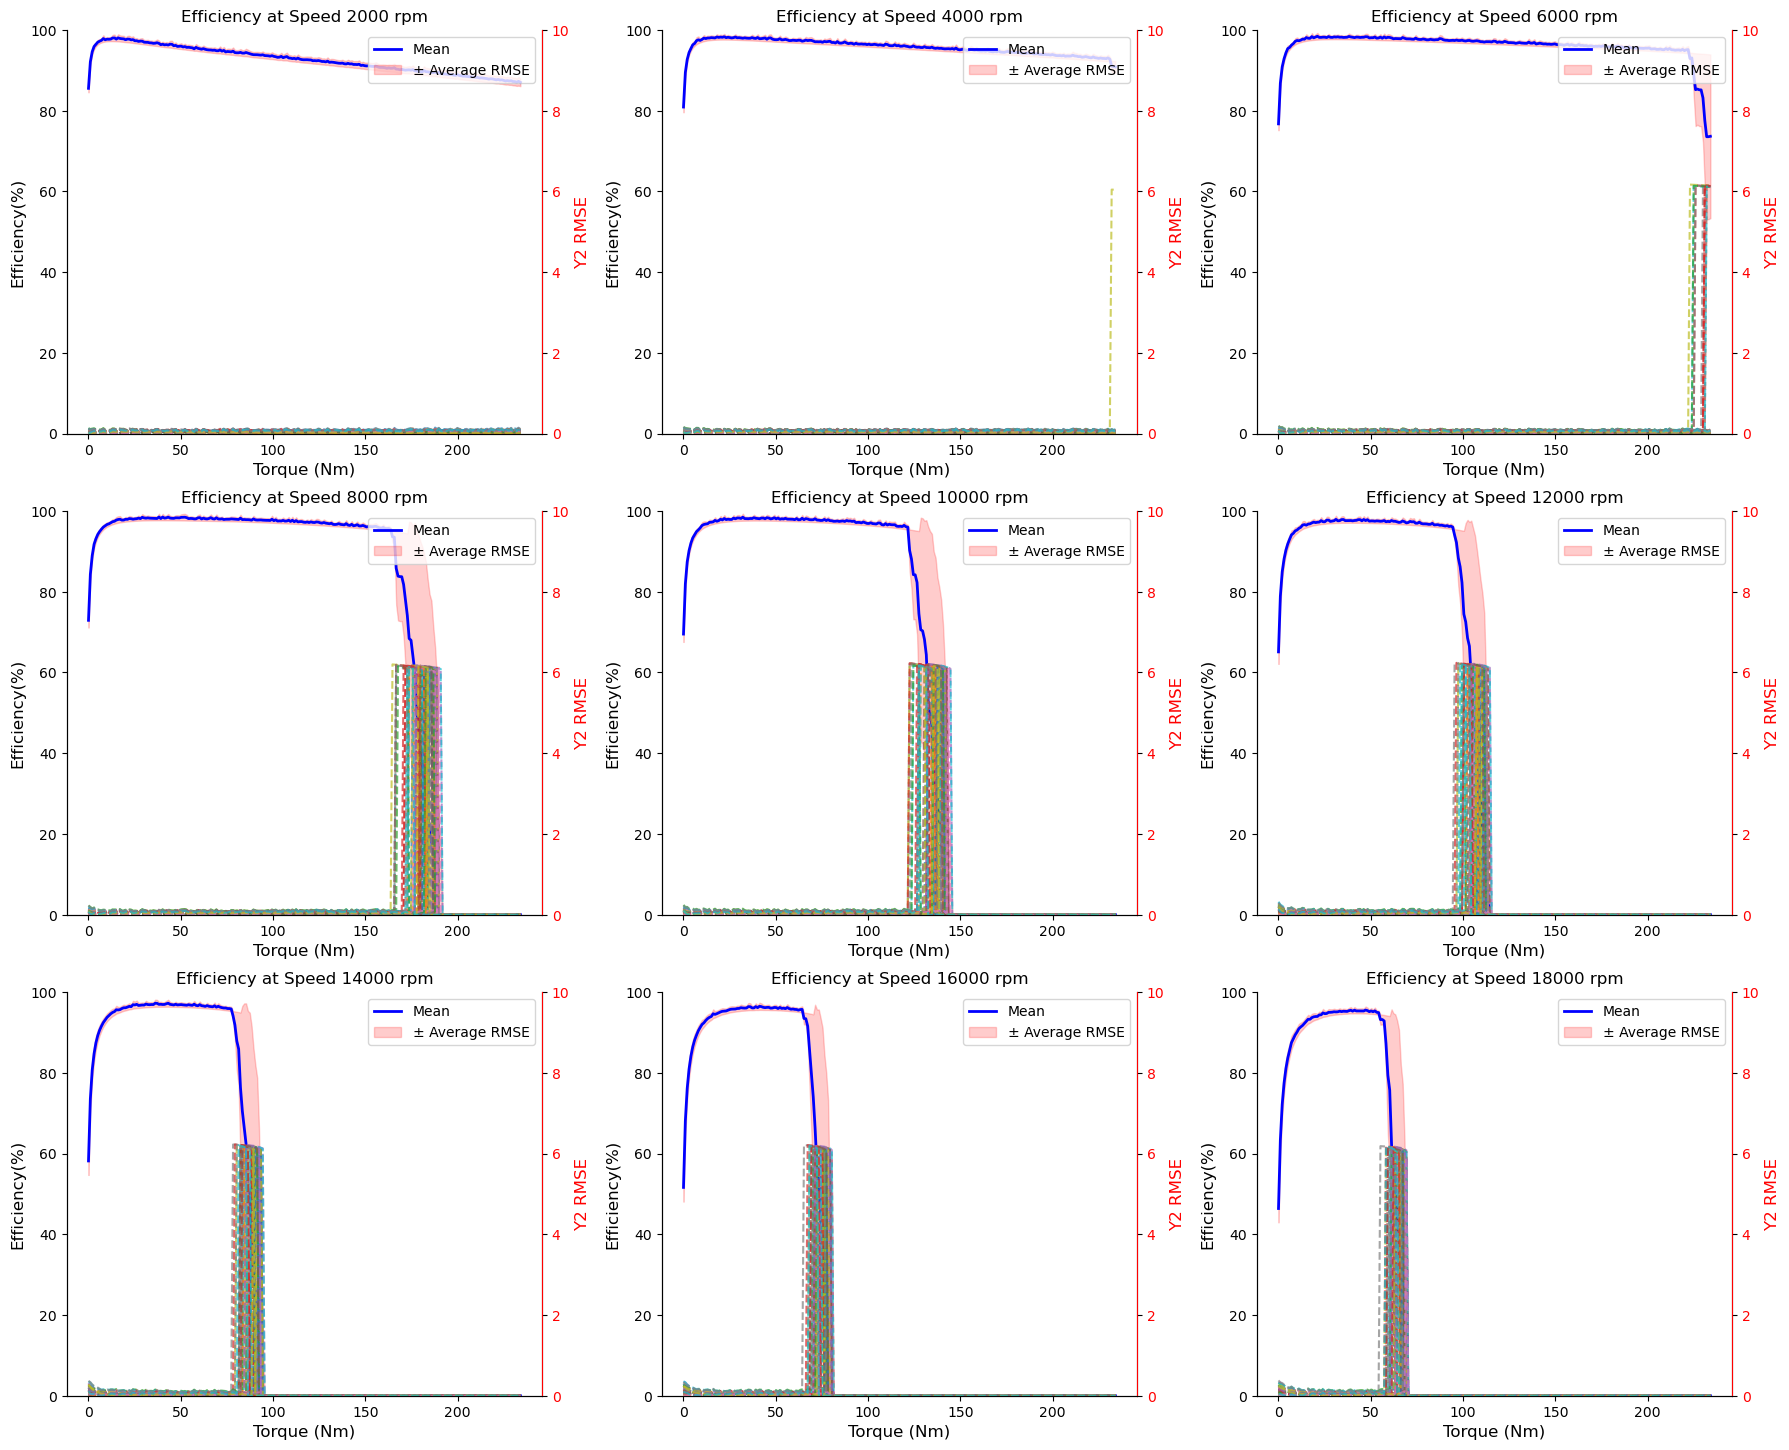
\includegraphics[width=1\textwidth]{./ReportImages/rmse_eta_MLP.png} 
    \caption{\ac{MLP} \ac{RMSE} Evaluation for Efficiency \ac{KPI}} 
    \label{fig:MLP RMSE Evaluation for Efficiency KPI}
\end{figure}

Efficiency \ac{KPI} is harder to evaluate scoring as it is 3\ac{D} with dimensions angular velocity, torque and efficiency. 
There exists 191 angular velocity ranges containing efficiency values.
Since it is infeasible to show the deviations of the efficiency with respect to all angular velocity intervals, I visualize the deviation with its respective targets 
only for certain angular velocities across the entire torque range in Fig. \ref{fig:MLP RMSE Evaluation for Efficiency KPI}. 
Therefore, the whole figure encompasses 6 subplots for specific angular velocities.\\
The figure shows the mean Efficiency values and the \ac{RMSE} surrounding it for 10 samples from the test dataset.
The angular velocities are chosen at equal intervals of 2000 rpm. The Efficiency values as usual range between 0 and 100\% percentage whereas the torque values are shown 
from 0 to approximately 250 Nm which could be the maximum torque value from the predictions of the handpicked samples.
The \ac{RMSE} of each prediction from its target can be viewed on the twin y-axis.\\

Fig. \ref{fig:Y2 Evaluation Statistics MLP} shows both the Fig. \ref{fig:Y2 RMSE} and Fig. \ref{fig:Y2 Percentage Difference} from Equations \ref{eq:Y2 Score} 
and \ref{eq:Y2 Percentage Difference} as histogram plots over the entire test dataset with the count of samples on the y-axis.
The histograms for both the figures are the same, nevertheless the intention is to be able to relate to the scores and percentage difference easily due to differing 
value ranges of the targets.
\begin{figure}[H]
    \centering
    \begin{subfigure}{0.5\textwidth}
        \centering
        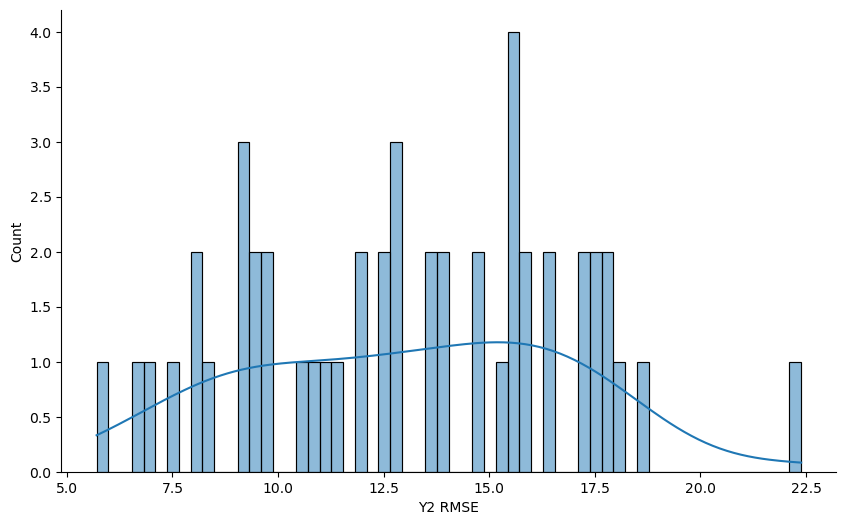
\includegraphics[width=\textwidth]{./ReportImages/score_MLP_y2.png}
        \caption{$\mathcal{Y}_2$ \ac{RMSE}}
        \label{fig:Y2 RMSE}
    \end{subfigure}\hfill
    \begin{subfigure}{0.5\textwidth}
        \centering
        \includegraphics[width=\textwidth]{./ReportImages/percentage_diff_MLP_y2.png}
        \caption{$\mathcal{Y}_2$ Percentage Difference}
        \label{fig:Y2 Percentage Difference}
    \end{subfigure}
    \caption{$\mathcal{Y}_2$ Evaluation Statistics of \ac{MLP}}
    \label{fig:Y2 Evaluation Statistics MLP}
\end{figure}

Fig. \ref{fig:MLP Training Deviation across Folds for Efficiency KPI} illustrates how each fold's prediction of efficiency deviates with the mean of the efficiency predictions 
of all folds against different angular velocities. Once again, to overcome the limitation of not being able to evaluate for all angular velocities, the Figure hosts only 6 
subplots for specific angular velocities. The evaluations is for the same target used in Fig. \ref{fig:MLP Training Deviation across Folds for Torque KPI} for all of the 5 folds.

\begin{figure}[H]
    \centering
    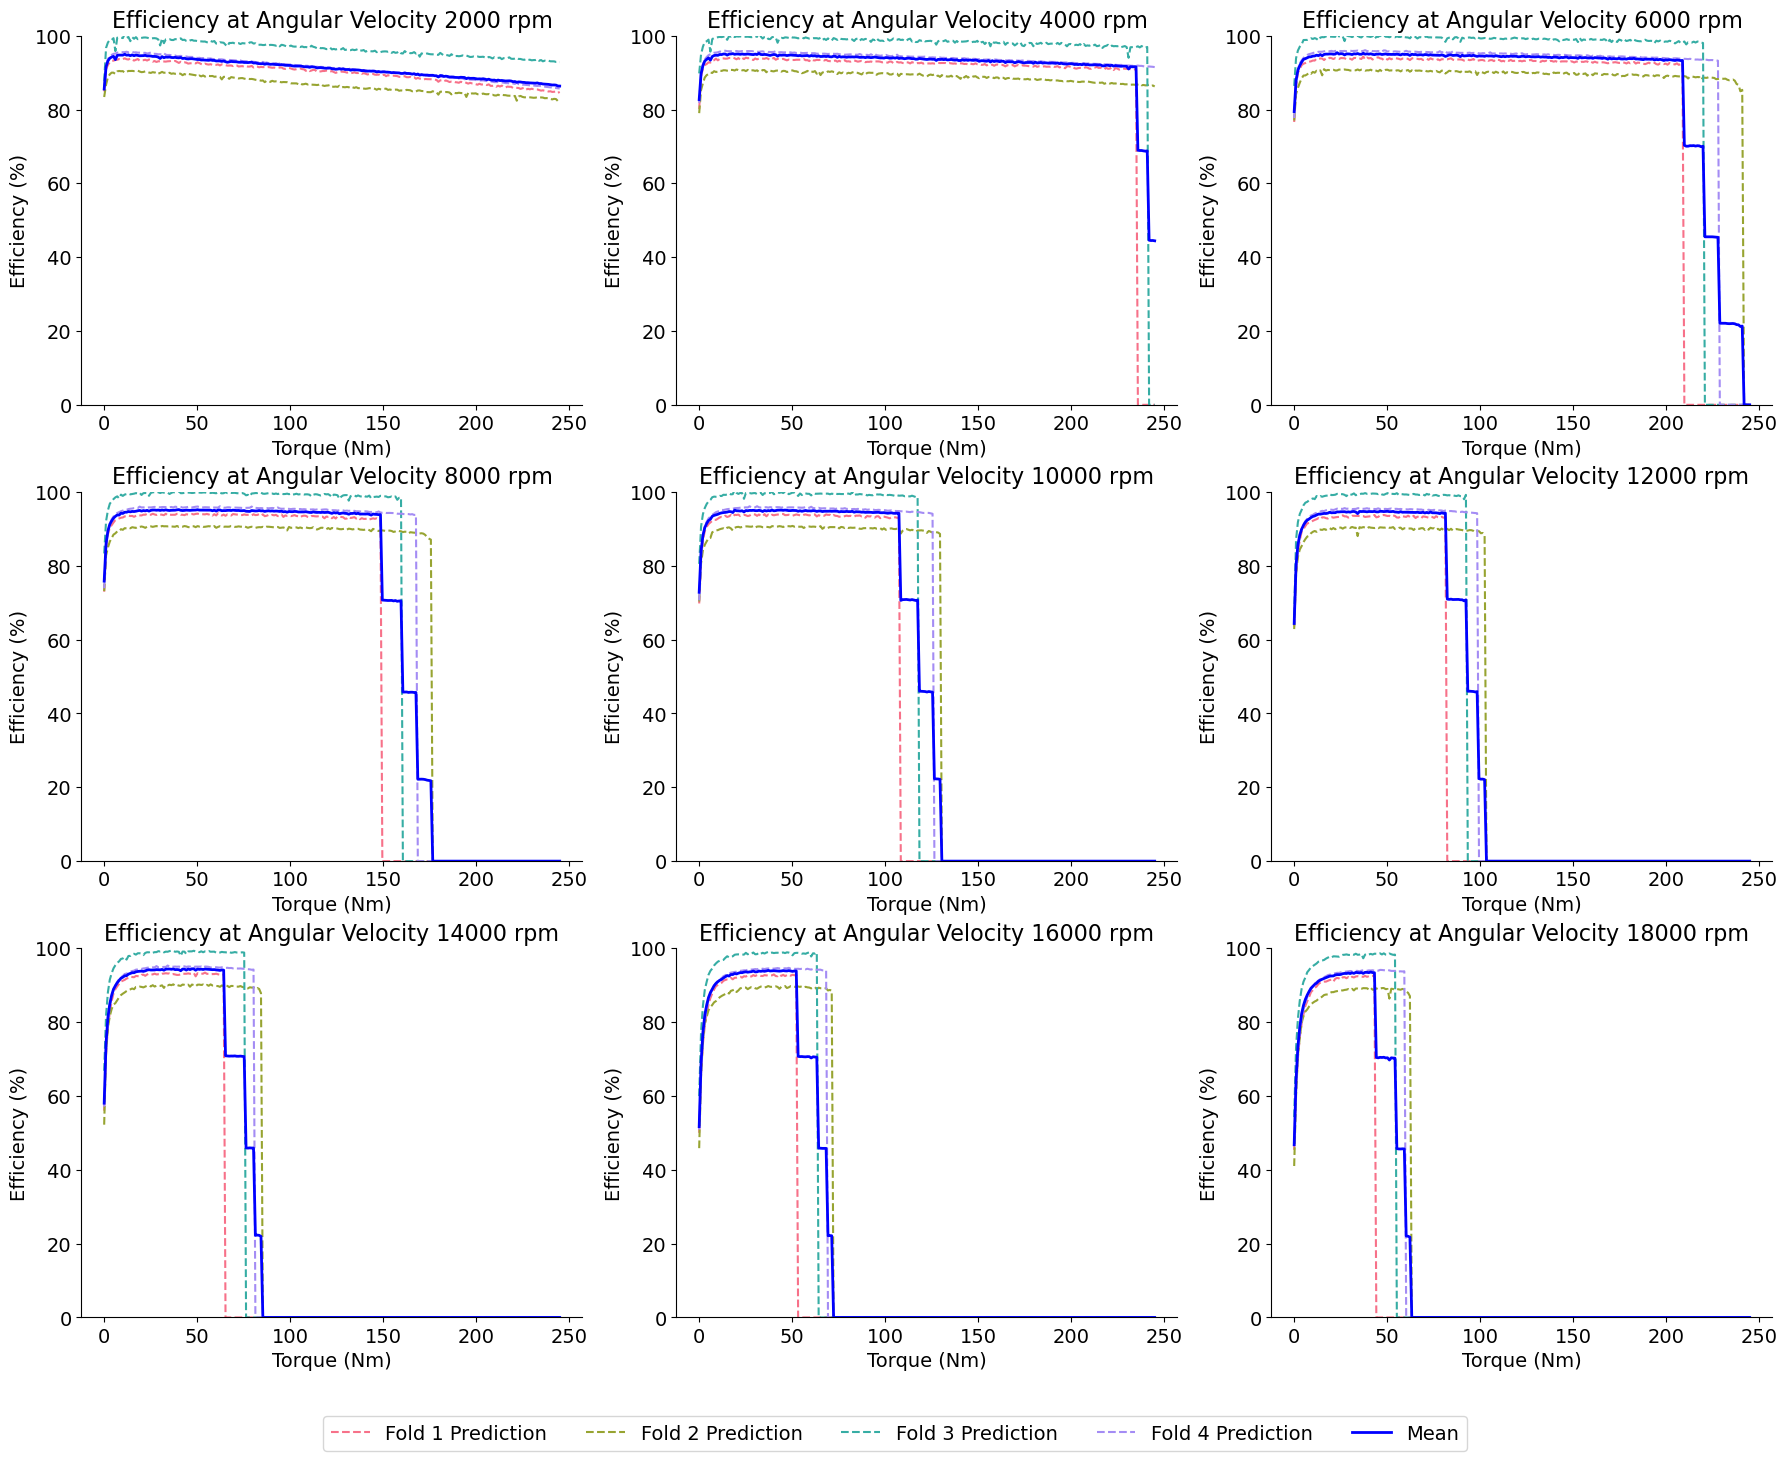
\includegraphics[width=1\textwidth]{./ReportImages/folds_dev_y2.png} 
    \caption{MLP Training Deviation across Folds for Efficiency \ac{KPI}} 
    \label{fig:MLP Training Deviation across Folds for Efficiency KPI}
\end{figure}

The following are the observations I infer of the Efficiency \ac{KPI} from the model:

\begin{enumerate}[nosep]
    \item Visually in Fig. \ref{fig:Efficiency KPI Predictions Vs Targets with MLP}, the predictions to a relative extent resembles the target and the regularization 
    of the Efficiency \ac{KPI} seems to be already teaching the model the nature of the Efficiency \ac{KPI}'s grid at extreme angular velocity and torque. 
    \item It can also be noted the efficiency values are being predicted well from the contours of the Efficiency grid.
    \item From Fig. \ref{fig:Efficiency KPI Predictions Vs Targets Vs Difference with MLP}, we can observe that for all 3 samples the difference highlighted is 
    the Efficiency Envelope aka Torque Curve being sliced off irregularly. This is the effect of us trying to retain the Torque \ac{KPI} shape as was 
    discussed in Section \ref{sec:Post Processing}.
    Additionally, it could be having negative impacts for the Efficiency \ac{KPI} when the predictions for the Torque \ac{KPI} are not perfect.
    This is yet again a decision to be made based on which of the 2 targets to prioritize with the weightage parameter\textit{$wt$}. MOVEEE!!!
    \item Additionally, the Fig. \ref{fig:Efficiency KPI Predictions Vs Targets with MLP}, Fig. \ref{fig:Efficiency KPI Predictions Vs Targets Vs Difference with MLP} would also 
    highlight the anomaly of efficiency values exceeding beyond 0-100\% if it occurs since the levels of the contours are fixed likewise. 
    Any values beyond this range would be visualized haphazardly.
    \item In comparison to Fig. \ref{fig:Standard Deviation of Efficiency KPI across Angular Velocity Intervals} it can be inferred that in Fig. 
    \ref{fig:MLP Standard Deviation of 3D KPI(Efficiency) across Angular Velocity Intervals with MLP}, the standard deviation of efficiency values predicted are slightly broader.
    \item Fig. \ref{fig:MLP RMSE Evaluation for Efficiency KPI} illustrates that for 1 sample the efficiency values compared to the other 9 samples \ac{RMSE} which appear 
    well approximated.  
    \item Another observation that can be made is that average \ac{RMSE} overlap along the Mean Efficiency is at its most towards the extreme torques across the 
    Efficiency envelope. The distinction is particularly prominent along the Efficiency envelope.
    \item However it is not only the border of the envelope a question of concern here but also for neighboring values of the envelope namely from 1/4th the 
    angular velocity onwards which is close to 6000 rpm. 
    I do not have any way to teach the model this part of the grid with loss regularization because I cannot estimate the envelope dimensionality having already padded 
    the targets to be of the maximum shape referred in Section \ref{subsec:Deep Dive into 3D KPI}. The reason why it deteriorates from 1/4th the angular velocity onwards is 
    because the Efficiency \ac{KPI}s envelope starts to converge from around 6000 rpm as can be seen in Fig. \ref{fig:Efficiency Grid}. 
    \item Additionally, I would like to point out from both Fig. \ref{fig:Standard Deviation of Efficiency KPI across Angular Velocity Intervals} and Fig. 
    \ref{fig:MLP RMSE Evaluation for Efficiency KPI} that the efficiency values do not exceed 100\% which makes it evident the outcomes of the regularization in Equation 
    \ref{eq:Y2 Maximum Efficiency Regularization}.
    \item It can be deduced from Fig. \ref{fig:Y2 Evaluation Statistics MLP} that the \ac{RMSE}s are gaussian distributed between 7-25 with the mean close to 14 thus 
    encompassing a range of 7-25\% percentage difference with the target values as derived from the Table \ref{tab:Scoring Criteria}.
    \item It can be remarked from Fig. \ref{fig:MLP Training Deviation across Folds for Efficiency KPI} that the predicted torque curves for all the folds except Fold 3 
    is as close as can be too each other in terms of efficiency values. However Fold 4, approximated the Efficiency envelope very different from the other folds. 
    As 3 folds approximation is close to each other,it indicates the model's generalization capability and its stability.
    \item To summarize the relatively higher errors are at located in the operating area along the shape of the torque curve.\\
\end{enumerate}

Observations from the predictions helped to correct few discrepancies in my development for instance in the Efficiency grid I replaced 0s with \ac{NaN} values which 
I later understood were both represented different in the grid. Since Efficiency values can take up values only between 0-100\%, I regard the same as constant 
across plots and use it as a baseline for determining the levels in the contour plot.

Additionally, I calculate the \ac{RMSE} and differences of prediction from the target by truncating the predicted and ground truth matrices to be of common shape.
I also replace \ac{NaN} values with 0s in either if it occurs as the Efficiency \ac{KPI}s were padded with \ac{NaN}s to be of the same shape but originally 
had no values as was discussed in Section \ref{subsec:Deep Dive into 3D KPI}. MOVE!!

\section{Results with Baseline}\label{sec:Results with Baseline}

From my observations on how the predictions closely resembled that of the target values in Section \ref{subsec:Deep Dive into 2D KPI} and 
Section \ref{subsec:Deep Dive into 3D KPI}, I have developed a Baseline model which is intrinsically the average of all samples of the training dataset.

\subsection{Torque KPI Results with Baseline}\label{subsec:Torque KPI Results with Baseline}

The $\mathcal{Y}_1$ Baseline score for the Efficiency \ac{KPI} can be formulated as shown in Equation \ref{eq:Y1 Baseline Score}.

\begin{equation}
    \text{$\mathcal{Y}_1$ Baseline Score} = \frac{1}{n} \sum_{i=1}^{n} \underbrace{ \sqrt{\frac{1}{h} \sum_{j=1}^{h} (\bar{y} - y_{ij})^2}}_{\mathcal{Y}_1\ Baseline\ RMSE},
    \label{eq:Y1 Baseline Score}
\end{equation}
where \(n\) is the number of \ac{EM} samples, \(\bar{y}\) is the Baseline Average mean, \(h\) is the columns of 1D vector, \(\mathcal{Y}_1\ Baseline\ \ac{RMSE}\) is the \ac{RMSE} for each test sample.\\

Fig. \ref{fig:Baseline RMSE Evaluation for 2D KPI(Torque)} shows the Average \ac{RMSE} and element wise \ac{RMSE} for the test dataset performance with the 
Baseline Model. The Figure is similar in structure to Fig. \ref{fig:MLP RMSE Evaluation for 2D KPI(Torque)}, however the distinction is in the values being displayed. 
Herein, the mean of the predictions from Baseline Model and \ac{RMSE} surrounding it is displayed for 10 samples from the test dataset. Additionally, in the twin y-axis, 
the \ac{RMSE} of the Baseline predictions from its target is shown in dotted lines.

\begin{figure}[H]
    \centering
    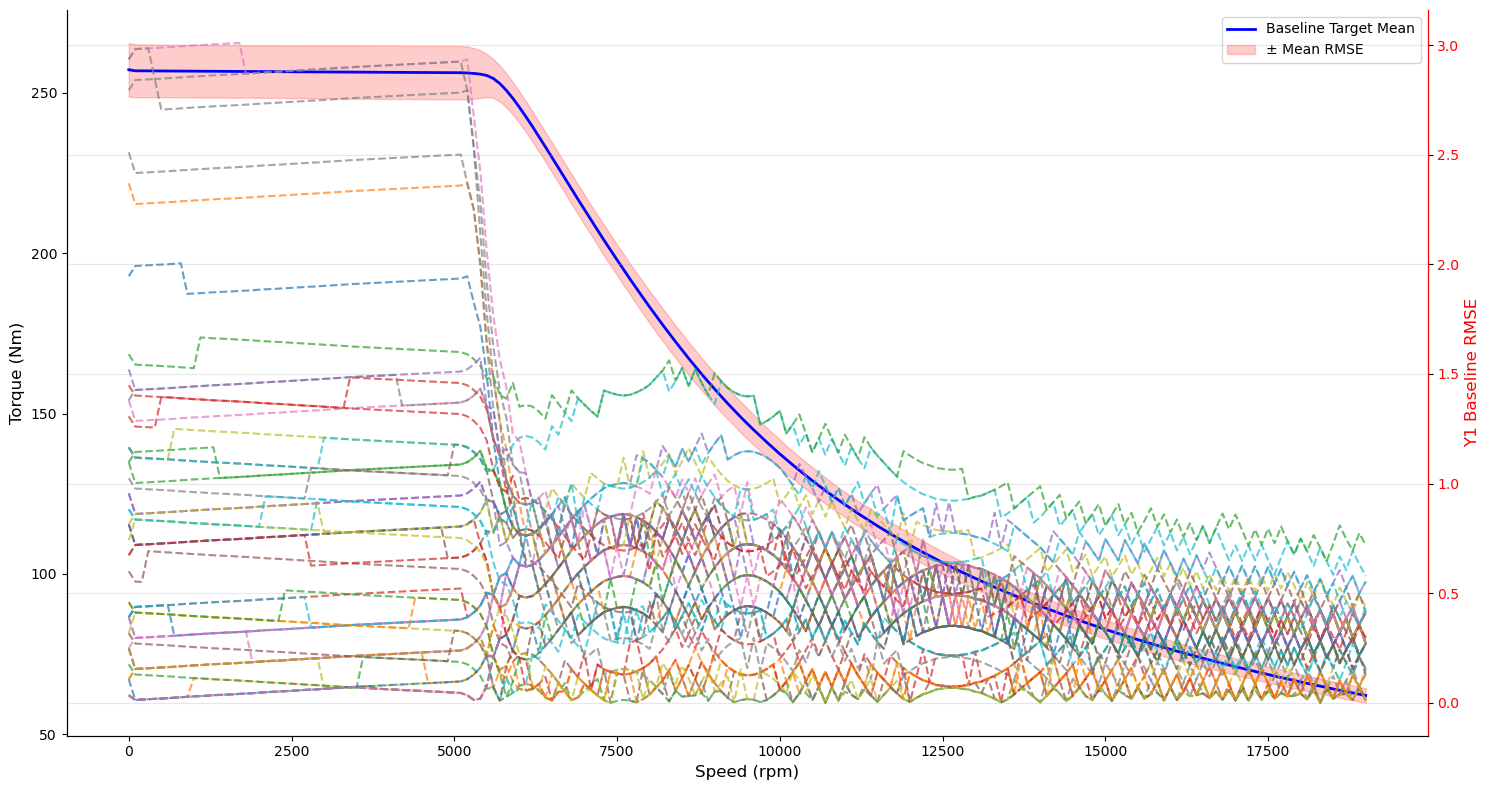
\includegraphics[width=0.6\textwidth]{./ReportImages/RMSE_Baseline_y1.png} 
    \caption{Baseline \ac{RMSE} Evaluation for Torque \ac{KPI}} 
    \label{fig:Baseline RMSE Evaluation for 2D KPI(Torque)}
\end{figure}

The following are the observations that can be inferred for the Torque \ac{KPI}:
\begin{enumerate}[nosep]
    
    \item In Fig. \ref{fig:Baseline RMSE Evaluation for 2D KPI(Torque)}, the deviations are at its most towards the beginning of the curve which steadily decreases along the curve.
    \item There are almost minimal fluctuations in the \ac{RMSE}s as compared to the predictions from the \ac{MLP} model in 
    Fig. \ref{fig:MLP RMSE Evaluation for 2D KPI(Torque)} for 1/4th of the initial angular velocities.
    \item Most importantly, it can be noted that \ac{RMSE} is at its highest soaring upto 6 compared to any of the \ac{MLP} models.\\
    This particular observation is the reason I believe the Baseline model will not serve as a good approximation of the Torque \ac{KPI}.\\
\end{enumerate}

\subsection{Efficiency KPI Results with Baseline}\label{subsec:Efficiency KPI Results with Baseline}

The $\mathcal{Y}_2$ Baseline score for the Efficiency \ac{KPI} can be expressed as shown in Equation \ref{eq:Y2 Baseline Score}.
\begin{equation}
    \text{$\mathcal{Y}_2$ Baseline Score} = \frac{1}{n} \sum_{i=1}^{n} \underbrace{ \sqrt{\frac{1}{w} \frac{1}{h} \sum_{j=1}^{w} \sum_{k=1}^{h} (\bar{y} - y_{ijk})^2}}_{\mathcal{Y}_2\ Baseline\ RMSE},
    \label{eq:Y2 Baseline Score}
\end{equation}
where \(w\) is the rows of 2\ac{D} vector, \(h\) is the columns of 2\ac{D} vector and \(\mathcal{Y}_2\ Baseline\ \ac{RMSE}\) is the \ac{RMSE} for each test sample.\\

Fig. \ref{fig:Baseline RMSE Evaluation for Efficiency KPI} gives a neat visualization of the Baseline Efficiency \ac{RMSE} with its respective targets for certain angular velocities  
across the entire torque range. This figure is yet again similar in structure to the Fig. \ref{fig:MLP RMSE Evaluation for Efficiency KPI} except that the efficiency values 
shown are the predictions of the Baseline model. \\

The following are the observations that can be inferred for the Efficiency \ac{KPI}:
\begin{enumerate}[nosep]
    \item The efficiency values are almost the same for more than 3/4th of the grid across the chosen samples. This is notable from observing the overlap of the 
    average \ac{RMSE} with the Mean Efficiency.
    \item However for the area along the Efficiency envelope, it can be noted that almost all samples have a deviation from the mean Efficiency values.
    \item The deviation at the Efficiency envelope is most prominent at lower angular velocities and gets better as the angular velocity increases.
    \item There are almost minimal fluctuations in the \ac{RMSE}s as compared to the predictions from the \ac{MLP} model in 
    Fig. \ref{fig:MLP RMSE Evaluation for 2D KPI(Torque)} for 1/4th of the initial angular velocities.
\end{enumerate}

\begin{figure}[H]
    \centering
    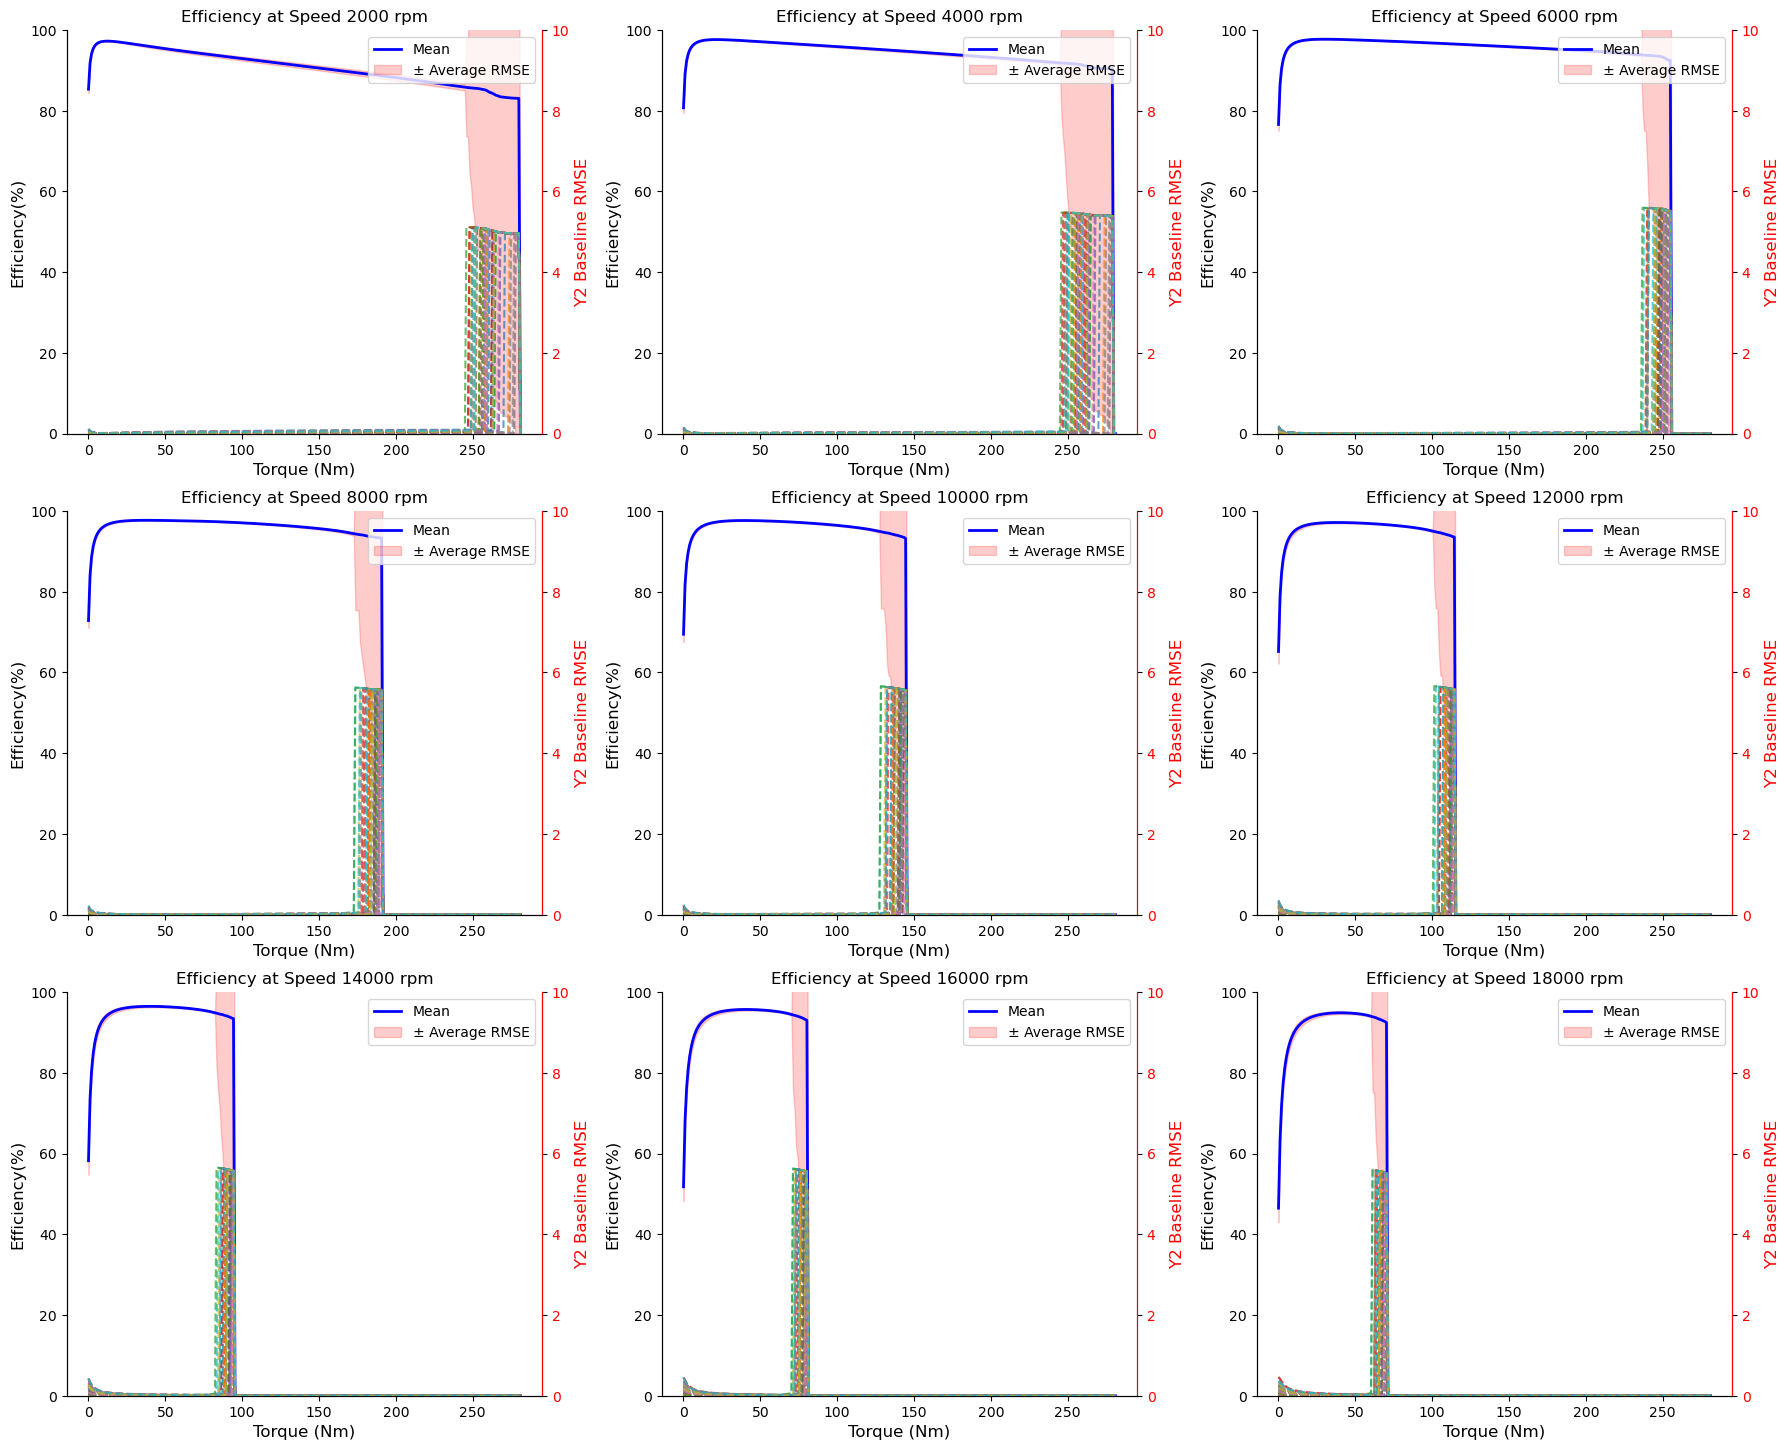
\includegraphics[width=1\textwidth]{./ReportImages/rmse_eta_Baseline.png} 
    \caption{Baseline \ac{RMSE} Evaluation for Efficiency \ac{KPI}} 
    \label{fig:Baseline RMSE Evaluation for Efficiency KPI}
\end{figure}

\section{Results with Torque KPI Loss Regularizations}\label{sec:Results with Torque KPI Loss Regularizations}

The model we have used here is the \ac{MLP} model with the Torque \ac{KPI} loss regularization terms.

\subsection{KPI Results with Smoothening Curve Loss Regularization}\label{subsec:KPI Results with Smoothening curve Loss Regularization}

The model I have used here is the \ac{MLP} model with the Torque \ac{KPI} with Smoothening Curve Loss Regularization discussed in 
Equation \ref{eq:Y1 Smoothening Loss Regularization}.

Fig. \ref{fig:Smoothening Torque RMSE Evaluation for 2D KPI(Torque)} shows the Average \ac{RMSE} and element wise \ac{RMSE} for 10 samples from the test dataset 
with the model. The structure of the figure is the same as Fig. \ref{fig:MLP RMSE Evaluation for 2D KPI(Torque)}.\\

The following are the observations that can be inferred for the Torque \ac{KPI}:
\begin{enumerate}[nosep]
    \item In Fig. \ref{fig:Smoothening Torque RMSE Evaluation for 2D KPI(Torque)}, it can be noted that \ac{RMSE} is considerably high compared to other models soaring upto 
    2.5
    \item Apart from the 2 samples which we expect the \ac{RMSE} to be high owing to them being outliers, 5 additional samples appear to also have a high \ac{RMSE}.
    \item The deviations are at its peak towards the beginning of the curve.
\end{enumerate}

\begin{figure}[H]
    \centering
    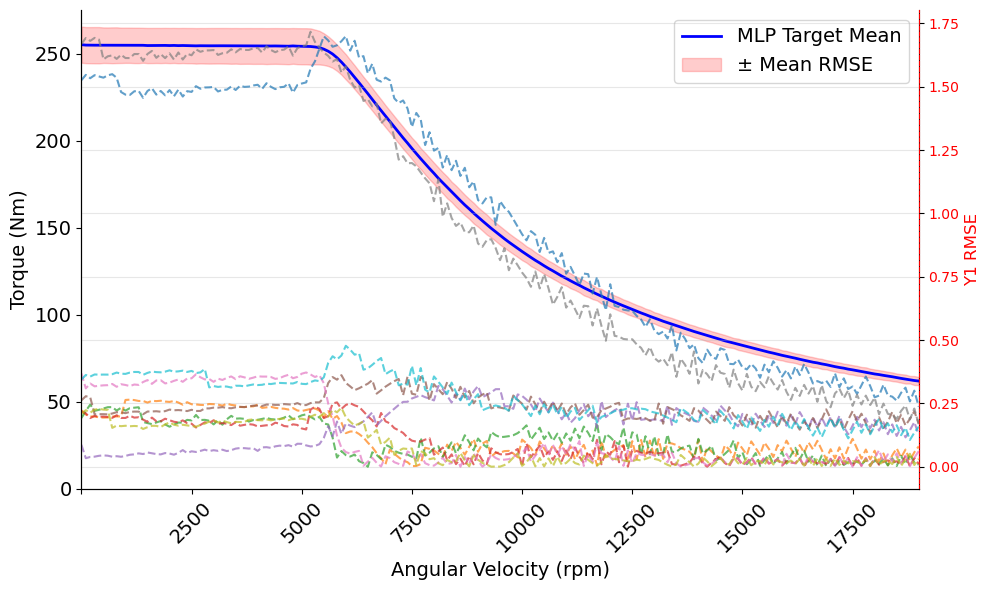
\includegraphics[width=0.6\textwidth]{./ReportImages/RMSE_MLP_Smoothening_y1.png} 
    \caption{Smoothening Curve \ac{RMSE} Evaluation for Torque \ac{KPI}} 
    \label{fig:Smoothening Torque RMSE Evaluation for 2D KPI(Torque)}
\end{figure}

\subsection{KPI Results with Decreasing Curve Loss Regularization}\label{subsec:KPI Results with Decreasing curve Loss Regularization}
The model I have used here is the \ac{MLP} Model with Decreasing Curve regularization discussed in Equation \ref{eq:Y1 Declining Loss Regularization}.

Fig. \ref{fig:Decreasing Torque RMSE Evaluation for 2D KPI(Torque)} shows the Average \ac{RMSE} and element wise \ac{RMSE} for few samples from the test dataset 
with the model. The structure of the figure is the same as Fig. \ref{fig:MLP RMSE Evaluation for 2D KPI(Torque)}.

The following are the observations that can be inferred for the Torque \ac{KPI}:
\begin{enumerate}[nosep]
    \item In Fig. \ref{fig:Decreasing Torque RMSE Evaluation for 2D KPI(Torque)}, it can be noted that \ac{RMSE} is considerably at its second high 
    ranging upto 2.
    \item Apart from the 2 samples which we expect the \ac{RMSE} to be high owing to them being outliers, 3 additional samples appear to also have a high \ac{RMSE}.
    \item The deviations are at its peak towards the beginning of the curve.
\end{enumerate}

\begin{figure}[H]
    \centering
    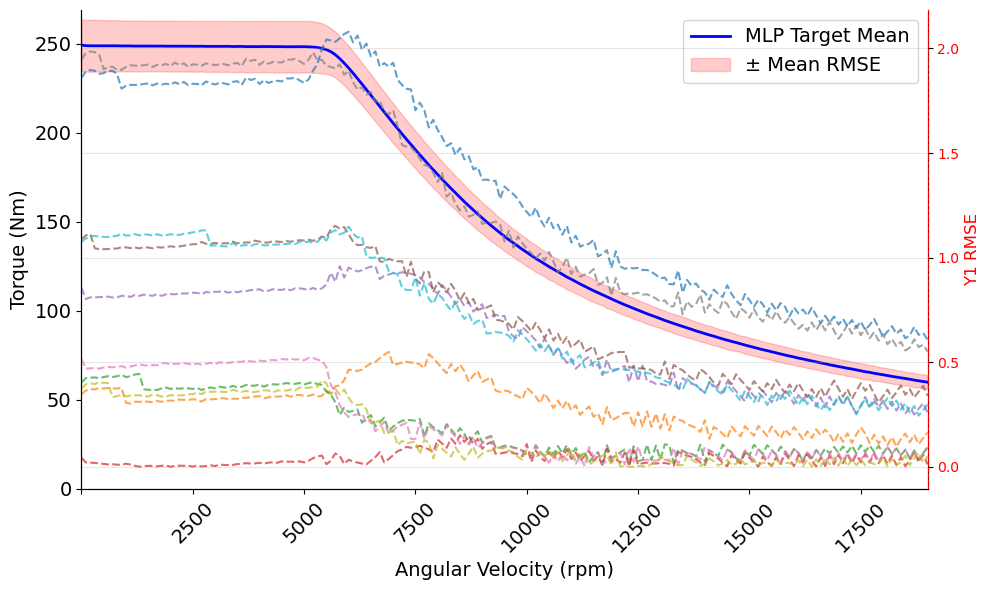
\includegraphics[width=0.6\textwidth]{./ReportImages/RMSE_MLP_Decreasing_y1.png} 
    \caption{Decreasing Curve \ac{RMSE} Evaluation for Torque \ac{KPI}} 
    \label{fig:Decreasing Torque RMSE Evaluation for 2D KPI(Torque)}
\end{figure}

\section{Results with No Loss Regularization}\label{sec:Results with No Loss Regularization}
The model we have used here is the \ac{MLP} model with any loss regularizations.

\subsection{Torque KPI Results with No Loss Regularization}\label{subsec:Torque KPI Results with No Loss Regularization}

Fig. \ref{fig:No Loss Regularization RMSE Evaluation for 2D KPI(Torque)} shows the Average \ac{RMSE} and element wise \ac{RMSE} for 10 samples from the test dataset 
performance with the model without any regularizations.

\begin{figure}[H]
    \centering
    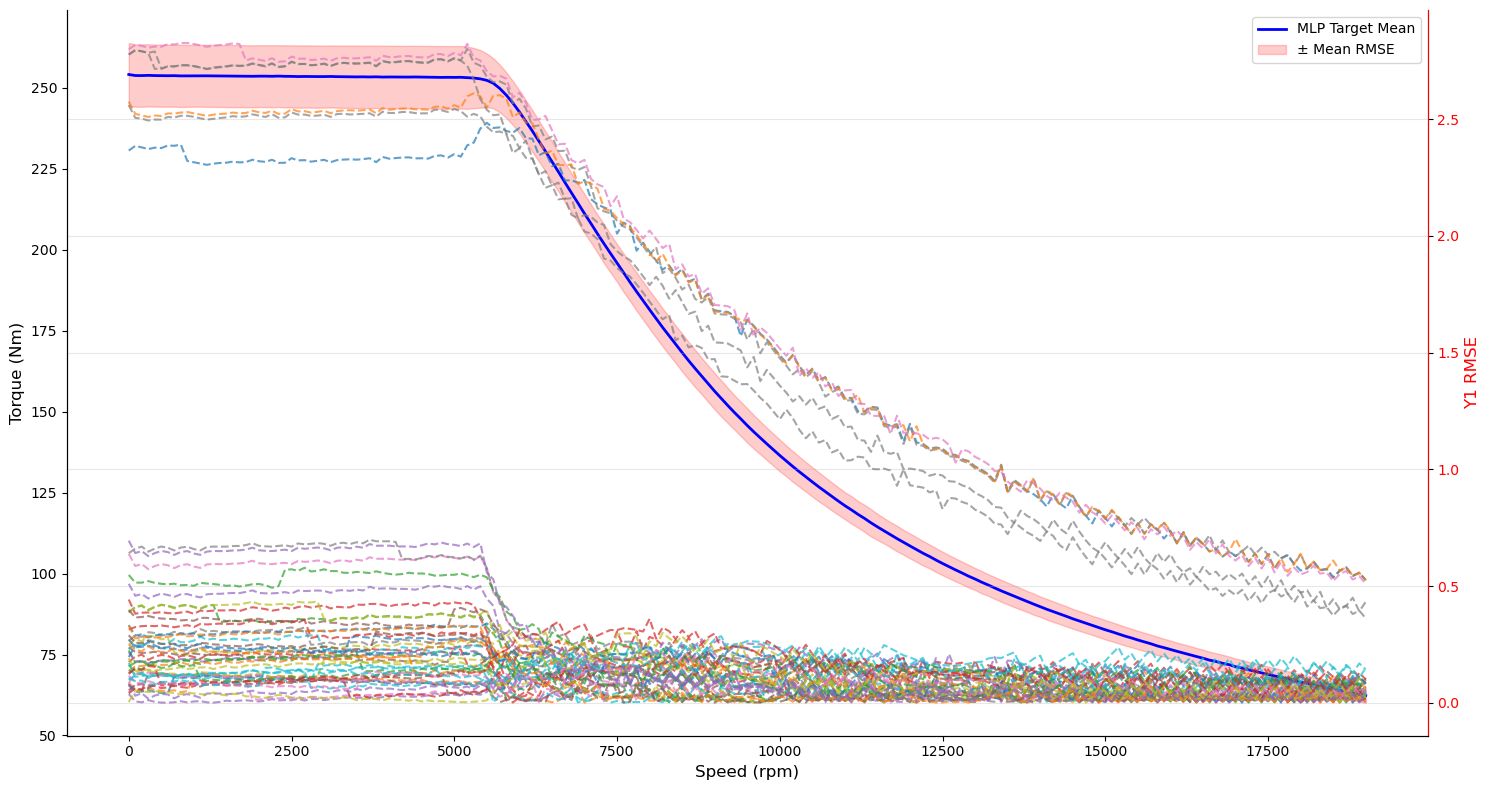
\includegraphics[width=0.6\textwidth]{./ReportImages/RMSE_MLP_no_lossreg_y1.png} 
    \caption{No Loss Regularization \ac{RMSE} Evaluation for Torque \ac{KPI}} 
    \label{fig:No Loss Regularization RMSE Evaluation for 2D KPI(Torque)}
\end{figure}

The following are the observations that can be inferred for the Torque \ac{KPI}:
\begin{enumerate}[nosep]
    \item In Fig. \ref{fig:No Loss Regularization RMSE Evaluation for 2D KPI(Torque)}, it can be noted that \ac{RMSE} is considerably the least among the other models.
    \item Apart from the 2 samples which we expect the \ac{RMSE} to be high owing to them being outliers, the other samples appear to be performing well in terms 
    of low \ac{RMSE}. This is a stark comparison to the Predictions with Loss Regularizations in Section \ref{sec:Results with Torque KPI Loss Regularizations}.
    \item The deviations are at its peak towards the beginning of the curve and gradually decrease when transitioning along the curve.
\end{enumerate}

\subsection{Efficiency KPI Results with No Loss Regularization}\label{subsec:Efficiency Results with No Loss Regularization}

Fig. \ref{fig:No Loss Regularization RMSE Evaluation for Efficiency KPI} gives a visualization of the Efficiency \ac{RMSE} with its respective targets 
for certain angular velocities across the entire torque range. The angular velocities are chosen at equal intervals of 2000 rpm.

The following are the observations that can be inferred for the Efficiency \ac{KPI}:
\begin{enumerate}[nosep]
    \item Similar patterns to the images generated with loss regularization in place can be remarked 
    in Fig \ref{fig:No Loss Regularization RMSE Evaluation for Efficiency KPI} with the \ac{RMSE} varying the most along the Efficiency envelope.
    \item However, on looking closely into Fig. \ref{KPI_Predictions_with_No_LossReg} and contrasting with the target Fig. \ref{Target KPIs}, it can be noted the efficiency 
    at low angular velocities do not have uniform coloring in blue at the border. This is representative of just 1 sample and on visual inspection of other samples, the fact that the 
    nature of the grid has not been captured becomes more visible in addition to efficiency values not conforming to be below 100\%.\\
\end{enumerate}

\begin{figure}[H]
    \centering
    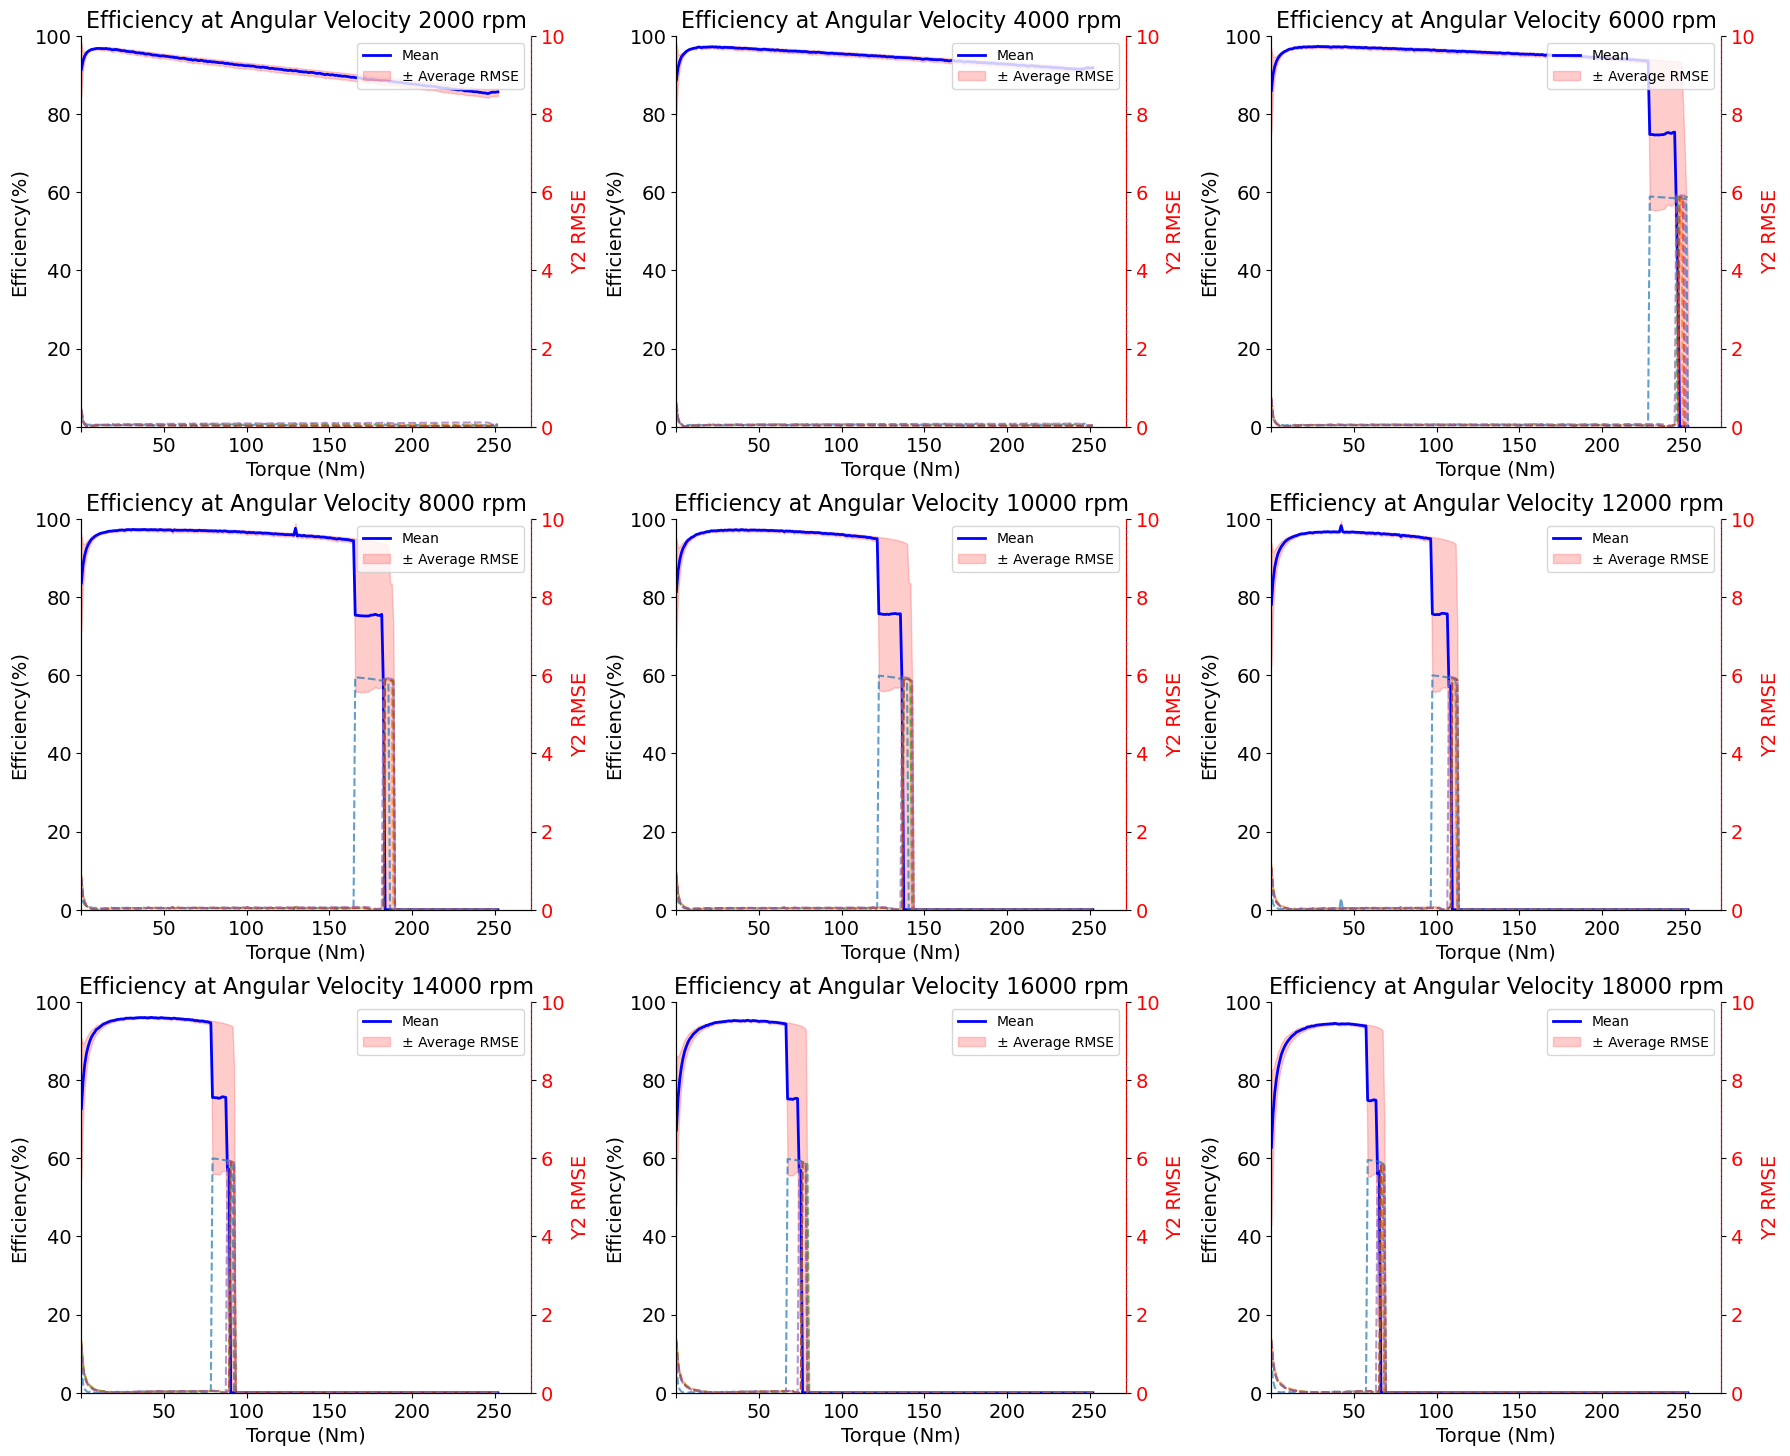
\includegraphics[width=1\textwidth]{./ReportImages/rmse_eta_no_lossreg_MLP.png} 
    \caption{No Loss Regularization \ac{RMSE} Evaluation for Efficiency \ac{KPI}} 
    \label{fig:No Loss Regularization RMSE Evaluation for Efficiency KPI}
\end{figure}

\section{Ablation Studies}\label{sec:Ablation Studies}

I conduct comprehensive ablation studies on the \ac{MLP} model with different loss regularizations and the Baseline model for both our targets.

\begin{minipage}[t]{\textwidth}
    \begin{table}[H]
        \centering
        \begin{tabular}{|p{0.275\textwidth}|p{0.275\textwidth}|p{0.275\textwidth}|}
        \hline {\bf Model} & {\bf $\mathcal{Y}_1$ Score} & {\bf $\mathcal{Y}_2$ Score}\\
        \hline 
        Baseline & 4.8201 & 15.3708 \\
        MLP\footnote{MLP with $\mathcal{Y}_2$ Loss Regularization} & 4.8552 & 13.6537  \\
        MLP\footnote{MLP With Decreasing curve $\mathcal{Y}_1$ Loss Regularization} & 6.7359 & 15.5493 \\
        MLP\footnote{MLP With Smoothening curve $\mathcal{Y}_1$ Loss Regularization} & 8.7409 & 14.3229 \\
        MLP\footnote{MLP without both $\mathcal{Y}_1$ and $\mathcal{Y}_2$ Loss Regularization} &  4.9058 & 15.5399  \\
        \hline
        \end{tabular}
        \caption{Ablation Studies}
        \label{tab:Ablation Studies}
    \end{table}
\end{minipage}

\vspace{1em} 

Results in Table \ref{tab:Ablation Studies} indicate that my \ac{MLP} model with only the Efficiency \ac{KPI} regularization's performance is in par with the 
Baseline model on the Torque \ac{KPI} and has outperformed it on the Efficiency \ac{KPI}. This could be because the regularizations are restrictive and discourage 
the model to learn better.
The enriched ablation studies I undertook demonstrate the robustness of the method across varying hyperparameter settings.\\

Additionally in Fig. \ref{fig:KPI Predictions for all Models for the same sample}, I generate \ac{KPI}s of 1 sample for all the models we developed to compare and contrast 
its predictions with the ground truth.\\

The following are the observations that can be inferred from the ablation studies:
\begin{enumerate}[nosep]
    \item The \ac{MLP} model with no loss regularization best approximates the Torque \ac{KPI} on visually checking the start of the curve.
    The \ac{MLP} models with loss regularizations appear to perform the worst in this regard.
    \item Visually, efficiency Values in Efficiency \ac{KPI} appear to be best for Baseline model and the \ac{MLP} model with Efficiency \ac{KPI} loss regularization.
    This is notable from the clear segregation of contours in the Efficiency maps. Although, the baseline model looks visually more appeasing yet it would be 
    wiser to trust the scoring as each color in the contour holds a range of values and finer details could be overlooked.
    \item For the \ac{MLP} models with no loss regularizations, the nature of the Efficiency grid as was mentioned already is not captured. 
    This particularity made me realize that the Efficiency grid regularization is good to have for the main model.
    \item For both the \ac{MLP} models with Torque \ac{KPI} regularizations, the torque values in the torque are not well approximated as is predicted to be much lower 
    than the actual values. This prompts us to exclude torque \ac{KPI} regularization from our main model.
    \item In addition, for the \ac{MLP} models with Decreasing Curve loss regularization, the efficiency grid appears to be cut off a lot, indicating that the 
    loss regularization forces the model to decrease the torque values more than required and could potentially be controlled with \textit{$\lambda_{2y1}$} parameter.\\
\end{enumerate}

The inferences shown are strictly speaking from the Double V Magnet Topology which assumed the bulk of the data I had received.
Considering the limitations in dataset, conducting thorough examinations of a substantial volume is typically unfeasible. 
Therefore, the primary purpose of the thesis is to study the possibility of modelling the \ac{KPI}s predictions and my learnings from it.

\section{Time Comparison}\label{sec:Time Comparison}

Table \ref{tab:Compute Time Comparisions} gives a glimpse of the time conserved with surrogate modelling and relates both the approaches highlighted in Fig. 
\ref{fig:EM Design Flowchart} in terms of time comparison and hardware requirements.

\begin{minipage}[t]{\textwidth}
    \begin{table}[H]
        \centering
        \begin{tabular}{|p{0.275\textwidth}|p{0.275\textwidth}|p{0.275\textwidth}|}
        \hline {\bf Approach} & {\bf Time taken(minutes)} & {\bf Hardware}\\
        \hline 
        Surrogate Modelling (Proposed Approach) & 18.5 seconds & 32 CPU Cores \& 1 GPU\\
        \ac{FEA} simulations (Current Approach)\footnote{Source : Valeo} & 5 minutes & 1500 CPU Cores\\
        \hline
        \end{tabular}
        \caption{Compute Time Comparison}
        \label{tab:Compute Time Comparisions}
    \end{table}
\end{minipage}

\vspace{1em} 

I would also like to bring to attention that the time of taking 5 minutes to generate \ac{KPI}s per design using the Current Approach highlighted in Fig. 
\ref{fig:EM Design Flowchart} is only possible by running the simulator across High Performance Computing machines of nearly 1500 CPU cores in parallel. 
As the number of cores decrease the simulation would take minutes to hours to converge. Additionally, it is the \ac{FEA} simulator in the block that is the culprit of 
consuming time. \\

Another pointer to note is in reality the time needed to generate \ac{KPI}s with Surrogate Modelling is in the range of milliseconds. 
However most time is utilized during the dataset creation in Data Preprocessing phase since reading the excel files to retrieve the tabular data takes up a 
significant chunk of time close to 18 seconds whereas only 5 seconds is required to generate the prediction and display both \ac{KPI}s.
The computing time of the \ac{ANN} surrogate models varied between 50.3 to 68 ms/case, which makes the surrogates 2,911 to 2,154 times faster than the FE reference simulation, 
respectively. CORRECT\\

As opposed to \ac{FEA} simulations, the time required to generate predictions for several motor designs is memory bound 
and computation is not so much of a bottleneck since I can potentially run both training and inference across multiple GPUs in parallel.\\

I have used Python 3.10.14 for my development and the \texttt{Pytorch}\footnote{\url{https://pytorch.org/}} Pytorch library compatible with Cuda.
The model was trained on a NVIDIA Tesla V100 \ac{GPU} with 32 GB Memory and the machine I used had 16 CPUs of the Intel(R) Xeon(R) Silver 4208 CPU @ 2.10GHz 
with allocated disk space of 50 GB for my experiments.
Source code is available at \texttt{\href{https://github.com/Lilly-25/Masters-Thesis}{Github Repository}}\footnote{\url{https://github.com/Lilly-25/Masters-Thesis}}.

\chapter{Graph Modelling} 

\section{Introduction}\label{sec:Introduction}

Tabular representation of data in itself cannot account for the spatiality of an \ac{EM} design especially on how its different components interact with one another. 
Meanwhile graphs thrive at better representing data in the non-Euclidean domain.
Therefore I presume modelling my usecase as a graph will be more reasonable so as to exploit its graph dynamics and aggregate features that are semantically similar.
This would be even more realistic with achieving topology invariance than the tabular representation and conserve memory and compute in the long run.\\

A graph can be composed of nodes and edges with their corresponding features in addition to the graph attributes.
The graph attributes contain the information relevant to the graph as a whole whereas the node features captures the information of the node's role in the network and 
likewise the edge features captures the information of the edge's role in the network. Graphs also take into account their respective neighborhoods.\\

On the basis of the directionality of edges within graphs, they can have the following taxonomy: Ref. \cite{GNN-2019}:
\begin{enumerate}[nosep]
    \item Directed Graph - A graph in which the edges have a direction from source node to its target node.
    \item Undirected Graph - A graph whose Adjacency matrix is symmetrical such that for each edge there will be its respective reverse edge in the opposite direction.
\end{enumerate}

In addition to their ability to incorporate both entity features and network features into a single, simultaneously trained model, most \ac{GNN}s scale linearly with 
the number of edges in the network, making them applicable to large networks.
Owerko \textit{et al.} demonstrate in Ref. \cite{PO GNN-2018} that power outages rely on sensors in the vicinity and can be attributed to weather conditions 
and so can be modelled using \ac{GNN}s. A hallmark of \ac{GNN}s is that they can efficiently learn the architecture parameters from the training data.\\

Researchers have broadly classified \ac{GNN}s following 2 distinct paradigms:
\begin{enumerate}[nosep]
    \item \textbf{Homogeneous \ac{GNN}} \\
        Homogeneous \ac{GNN} are designed for graphs with a single type of nodes and edges. 
        \ac{MP} is done for neighbouring nodes and edges over hops until it learns a representation equivalent from its neighbours.
        Homogeneous \ac{GNN} are typically build to capture the structural information within a graph.
        These models are effective when the node and edge heterogeneity is negligible as stated by the authors of Ref. \cite{EHR HGNN-2024}. 
    \item \textbf{Heterogeneous \ac{GNN}} \\    
        Heterogeneous \ac{GNN} are designed for graphs with differing types of nodes and edges implying difference in features as well as dimensionality.
        The authors of Ref. \cite{{HNNC-2023}} argue that each type of node and edge reveal unique semantic information.
        As a single function cannot cater to each type, hence different \ac{MP} and node updating functions needs to be implemented for each edge and node type respectively.
        Therefore \ac{MP} is conditioned on the node and edge type thus allowing the flow of information to be more controlled. 
        In addition to the structural information, Heterogeneous \ac{GNN}s also excel to capture semantic information within the graph.\\
\end{enumerate}

\begin{figure}[H]
    \centering
    \begin{subfigure}{0.35\textwidth}
        \centering
        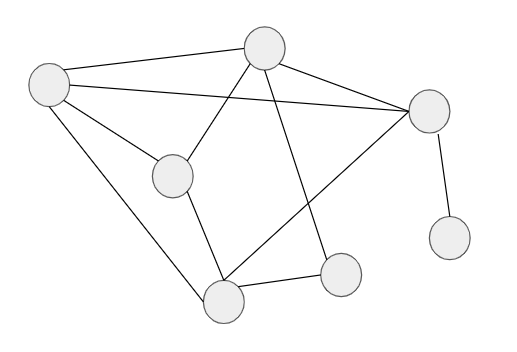
\includegraphics[width=\textwidth]{./ReportImages/HomogeneousGraph.png}
        \caption{Homogeneous Graph} % Center the caption here
        \label{fig:Homogeneous Graph}
    \end{subfigure}
    \begin{subfigure}{0.35\textwidth}
        \centering
        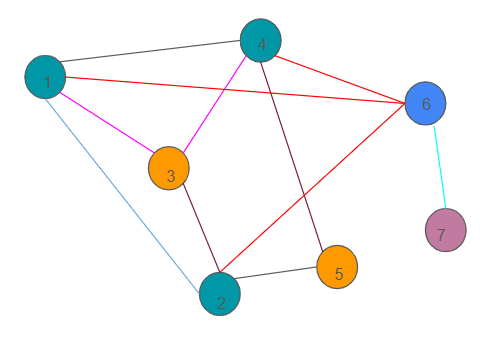
\includegraphics[width=\textwidth]{./ReportImages/HeterogeneousGraph.png}
        \caption{Heterogeneous Graph}
        \label{fig:Heterogeneous Graph}
    \end{subfigure}
    \caption{Graph Classification}
    \label{fig:Graph Classification}
\end{figure}
Fig. \ref{fig:Graph Classification} distinguishes the 2 graphs with equivalent number of nodes and edges by the coloring used for different nodes and edges they possess. 
Fig. \ref{fig:Heterogeneous Graph} comprises of 6 edge types and 4 node types whereas Fig. \ref{fig:Heterogeneous Graph} comprises of just 1 node type and edge type.

\subsection{Message Passing}\label{subsec:MP}

\ac{GNN}s in general function by making use of \ac{MP} which is a recursive algorithm that aims to learn a representation vector for each node. 
\ac{MP} is based on the graph structure and initial features per node. Over each hop of successive neighborhoods in the graph, the information of neighboring nodes are 
shared across as messages and aggregated and the initial node is recursively updated with this information. This continues until there are left no more nodes to traverse 
within the graph. Thus, at the end of the \ac{MP} algorithm, each node in the graph would have a good understanding of the other nodes within the same graph.
Therefore, the final representation will be rich enough to have captured all the information within the graph and can be used for downstream tasks.\\

Fig. \ref{fig:Message Passing} illustrates the working of \ac{MP} in a homogeneous graph of 7 nodes and 11 edges. Fig. \ref{fig:Message Passing for whole graph} shows 
the effect of \ac{MP} for all nodes in the graph  whereas Fig. \ref{fig:Message Passing for 1 Node} zooms in on the effect of \ac{MP} for a single node in the graph.
The neigboring node vectors of node 1 are aggregated and updated to node 1's vector. Aggregation is made visually understandable by color coding each node's respective 
vector representation distinctly and node updation is made obvious by updating its respective color to the vector index corresponding to the node number. 

\begin{figure}[H]
    \centering
    \begin{subfigure}{\textwidth}
        \centering
        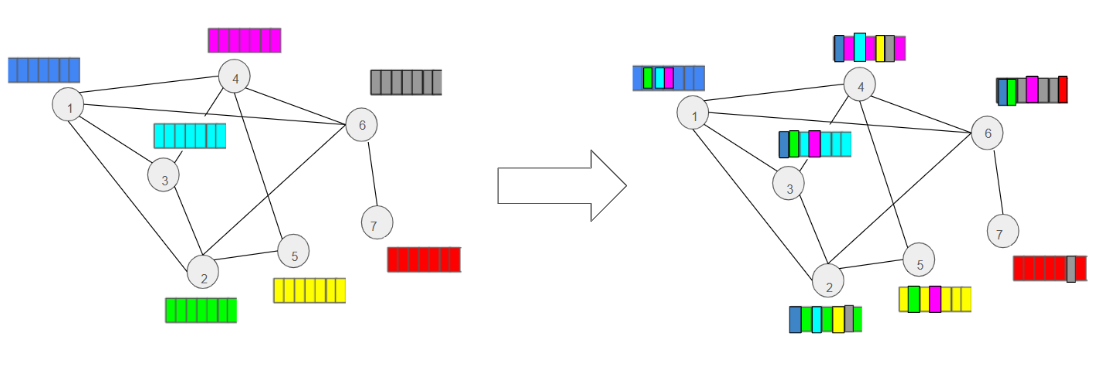
\includegraphics[width=.9\textwidth]{./ReportImages/HomogeneousMP.png} 
        \caption{Message Passing for whole graph} 
        \label{fig:Message Passing for whole graph}
    \end{subfigure}\vfill
    \begin{subfigure}{\textwidth}
        \centering
        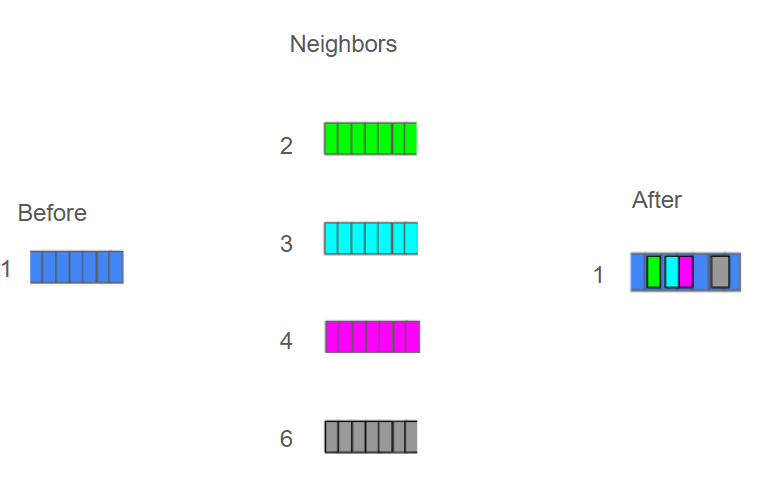
\includegraphics[width=0.35\textwidth]{./ReportImages/HomogeneousMP1Node.png}
        \caption{Heterogeneous Graph}
        \label{fig:Message Passing for 1 Node}
    \end{subfigure}
    \caption{Message Passing}
    \label{fig:Message Passing}
\end{figure}

\ac{GNN}s cannot be too deep with layers due to the oversmoothing problem. 
Oversmoothing is said to have occurred when the \ac{MP} algorithm would have already traversed over all hops and made all node features indistinguishable from one another.
Besides a deep \ac{GNN} would have a large number of parameters and would be computationally expensive to train.

\subsection{Applications}\label{subsec:Applications}

Some of the well known \ac{GNN} tasks can be seen in Fig. \ref{fig:GNN Predictions} :
\begin{enumerate}
    \item Graph Classification - Used for classifying graphs into different categories. Although our usecase is a Graph level Prediction, it is a graph multi-regression 
    task as we need to predict continuous values as was clarifed in Section \ref{sec:Objective}
    \item Node Classification - A node's class is predicted based on its proximity with other nodes in its neighborhood. An application could be in Named Entity 
    Recognition tasks for Knowledge graphs.
    \item Link Prediction - Predict whether there exists relationships between nodes in the graph. A common application is predicting drug treatment based on gene-protein interactions.
    \item Community Detection - Classifies groups of nodes into clusters. One scenario of application is to detect mutual communities in a social network.
    \item Graph Embedding - Embeds high dimensional graph into a lower dimensional space to be able to visually inspect it better. Visualizing huge corpus of text as 
    Knowledge graph in lower dimension, enables one to detect communities of topics and subtopics in each cluster.
    \item Graph Generation - Generates synthetic graphs based on initial graph representation. An application I can relate to is the inverse formulation of our problem 
    modelled as a graph which can be envisioned in the future discussed in Section \ref{sec:Motivation}.
\end{enumerate}

\begin{figure}[H]
    \centering
    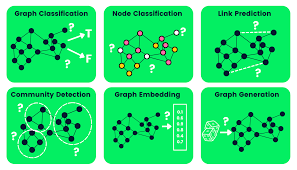
\includegraphics[width=0.5\textwidth]{./ReportImages/GraphTasks.png} 
    \caption{\ac{GNN} Tasks (Source : https://www.datacamp.com/tutorial/comprehensive-introduction-graph-neural-networks-gnns-tutorial) }
    \label{fig:GNN Predictions}
\end{figure}

\ac{GNN}s have several applications where data are generated from non-Euclidean domains and are represented as graphs with complex relationships 
and interdependency between objects Ref. \cite{GNN-2019}.
These networks are generally represented by a giant graph in which case graph batching, splitting are unique. However our task requires us to build 1 graph each for each \ac{EM} variant.

\subsection{Case Study Structure}\label{subsec:Case Study Structure}
I have organized the outline of the case study to be as follows:
First, I provide an introduction on \ac{GNN}s in Introduction.
I then delve into finer details of the Heterogeneous \ac{GNN}s in Section \ref{sec:Heterogeneous GNN} and formulate definitions mathematically.
Next, I review Literature done on Heterogeneous \ac{GNN}s in Section \ref{sec:HGNN Literature Review}.
After which I present the methodology in Section \ref{sec:EM Heterogeneous GNN Model} and share our view on how to create the heterogeneous graph for our usecase.
Lastly, I wrap up with a brief discussion of the pros and cons of using heterogeneous \ac{GNN}s in Section \ref{sec:EM Heterogeneous GNN Discussion}.

\section{Heterogeneous GNN}\label{sec:Heterogeneous GNN}

Graphs are ubiquitously heterogeneous because of its capability to have different node and edge types on top of its inherent graph feature to abstract and model 
relations between objects.
Heterogeneous \ac{GNN}s also takes into account homophily wherein nodes close on a network have similar embeddings Ref. \cite{HGNN-2020} this is in essence the structural 
property and is true for all \ac{GNN}s. I largely adopt the commonly used notations from Ref. \cite{ML HGNN-2023} and reformulate it slightly for our task. \\

\textbf{Heterogeneous Networks}

Given a directed graph \( \mathcal{H} = (V, E, X, R, T_v, T_e, \phi, \psi) \), 
where \( V \) is the set of nodes, \( E \) is the set of edges, \( X \) is the set of node features, \( R \) is the set of edge features,

The sets of possible node types can be represented as: \( T_v = \{ \phi(v) : \forall v \in V \} \) and the sets of possible edge types 
can be represented as: \( T_e = \{ \psi(e) : \forall e \in E \}.\) 

Each node \( v \in V \) has a node type \( \varphi(v) = \nu \in T_v \), where \( \varphi(\cdot) \) is a node type mapping function. 
Furthermore, for \( \varphi(v) = \nu \), \( v \) has features \( x_v^{\nu} \in X^{\nu} \), 
where \( X^{\nu} = \{ x_v^{\nu} \mid v \in V, \varphi(v) = \nu \} \) and \( X = \{ X^{\nu} \mid \nu \in T_v \} \). 
The dimension and attributes of the node feature \( x_v^{\nu} \) may be different for different node types \( \nu \). 

Each edge \( e_{uv}^{\varepsilon} \) has an edge type \( \varepsilon \in T_e \) pointing from node \( u \) to \( v \). 
Each edge \( e_{uv}^{\varepsilon} \) has features \( r_{uv}^{\varepsilon} \in R^{\varepsilon} \), 
where \( R^{\varepsilon} = \{ r_{uv}^{\varepsilon} \mid u, v \in V \} \) and \( R = \{ R^{\varepsilon} \mid \varepsilon \in T_e \} \). 
Similar to nodes, the edge features can have different dimensions and attributes for different edge types.

If \( |T_v| = |T_e| = 1 \), it implies there is only 1 node and edge type then the graph degenerates into a homogeneous graph stated by authors of Ref. \cite{SE HGNN-2023}.

Heterogeneous \ac{GNN}s aim to learn a representation vector \( \mathbf{h}^{(L)}_v \in \mathbb{R}^{d_L} \) for each node \( v \) after \( L \)-layer transformations, 
based on the graph structure and the initial node feature \( \mathbf{h}^{(0)}_v \in \mathbb{R}^{d_0} \) Ref. \cite{REF HGNN-2021}.\\

Fig. \ref{fig:Heterogeneous GNN Terminologies} illustrates each of the below terminologies to relate better.  \\

\textbf{Metarelation}

For an edge \( e = (s, t) \) linking source node \( s \) to target node \( t \), its meta relation is denoted as $\langle \varphi(s), \psi(e), \varphi(t) \rangle.$
Metarelations are the relation triples used in knowledge graphs as it contains richer schema. \\

\textbf{Metapath}

Metapaths are composite relationships between nodes that help to capture the structural information of heterogeneous graphs.

Given a path $\mathcal{P} = T_{v1} \xrightarrow{T_{e1}} T_{v2} \xrightarrow{T_{e2}} \cdots \xrightarrow{T_{el}} T_{vl}$, 
if the path describes the composition of edges by its types \( T_{e1} \circ T_{e2} \circ \cdots \circ T_{el} \) between nodes of type \( T_{v1} \) and \( T_{vl} \) and 
$\circ$ denotes the composition operator then the path is called a metapath. 

The length of the metapath can be calculated from its magnitude i.e, \textit{l-1}. 
The metapath is also the sequence of many metarelations.  If all the combinations of nodes and edges in the graph are used, then the total number of metapaths would 
increase exponentially with the number of node and edge types. Hence, the reason to subselect only few metapaths that are significantly most relevant for the task at hand. 

Metapath selection requires domain knowledge to be able to choose those which are most semantically meaningfull and let the Heterogeneous \ac{GNN} use only these paths 
for learning the graph.  Thus metapaths control the direction of message passing in a neural network.\\

The Metapaths in Heterogeneous \ac{GNN}s are divided into 2 streams:
\begin{enumerate}[nosep]
    \item Metapath based method\\
    It strictly follows the metapaths defined for the network.
    Each metapath is assumed to be unique in terms of its semantic meaning, therefore this method aggregates inforamtion from each metapath before fusing 
    information of other metapaths that are not so much semantically related.
    \item Metapath free method\\
    There are no metapaths defined for the network and so this method attempts to learn from the graph structure.
    It aggregates message from neighbourhood of the same hop for all node types and so captures both structural and semantic information simultaneously.
\end{enumerate}

Multiple \ac{MP} operations are done across different metapaths which are finally aggregated into a new representation for the node.Ref. \cite{ML HGNN-2023}.
Each metapath captures the proximity of nodes in a graph from a specific semantic view Ref. \cite{HGNN-2020}. \\

\textbf{Metapath-based Neighbors}

Given a node $v_1$ and a meta-path $\mathcal{P}$ in a heterogeneous graph, the neighbors \( \mathcal{N}_{v_1}^{\mathcal{P}} \) of 
node $v_1$ along the meta-path $\mathcal{P}$ are defined as the set of nodes connected to $ v_1$ including $v_1$ via the meta-path $\mathcal{P}$. \\

\textbf{Metapath-based Subgraph}

Given a heterogeneous graph, $\mathcal{H}$ with a metapath, $\mathcal{P}$, then the metapath-based subgraph, $\mathcal{H_P}$, is defined as a graph consisting of all 
its metapath based neighbors. Moreover, $\mathcal{H_P}$ degenerates to a homogeneous subgraph if $\mathcal{P}$ is symmetric.\\

Heterogeneous \ac{GNN} generally work by having separate non linear functions convolve over each edge type during message computation and over each node type when 
aggregating the learned information. 

The graph structure of $\mathcal{H}$  can be represented by a series of adjacency matrices \(\{A_\varepsilon : \varepsilon \in T_e\}\). 
For each relation \(\varepsilon_{\nu_t \nu_s} \in R\), \(A_{\nu_t \nu_s} \in \mathbb{R}^{|V_{\nu_t}| \times |V_{\nu_s}|}\) is the corresponding 
adjacency matrix where the nonzero values indicate positions of edges \(E_{\nu_t \nu_s}\) of the current relation.\\
% During runtime, the \ac{MP}-\ac{GNN} algorithm would need to iterate over edge type dictionaries during message computation and over node type dictionaries during node updates.

\begin{figure}[H]
    \centering
    \begin{subfigure}{0.35\textwidth}
        \centering
        \includegraphics[width=\textwidth]{./ReportImages/Metapath.png}
        \caption{Metapath} 
        \label{fig:Metapath}
    \end{subfigure}\hfill
    \begin{subfigure}{0.35\textwidth}
        \centering
        \includegraphics[width=\textwidth]{./ReportImages/Metarelation.png}
        \caption{Metarelation}
        \label{fig:Metarelation}
    \end{subfigure}\vfill
    \begin{subfigure}{0.35\textwidth}
        \centering
        \includegraphics[width=\textwidth]{./ReportImages/MetapathNeighbors.png}
        \caption{Metapath based Neighbors} % Center the caption here
        \label{fig:MetapathNeighbors}
    \end{subfigure}\hfill
    \begin{subfigure}{0.35\textwidth}
        \centering
        \includegraphics[width=\textwidth]{./ReportImages/Metasubgraph.png}
        \caption{Metapath based Subgraph}
        \label{fig:Metasubgraph}
    \end{subfigure}
    \caption{Heterogeneous \ac{GNN} Terminologies}
    \label{fig:Heterogeneous GNN Terminologies}
\end{figure}

\section{GNN Literature Review}\label{sec:HGNN Literature Review}
I try to review the recent works on Heterogeneous \ac{GNN} by categorizing them across the following subsections:

\subsection{Metapaths}\label{subsec:HGNN Metapaths}
Xu \textit{et al.} in Ref. \cite{EMPHGNN-2023} demonstrated a technique of splitting metapaths from inside out to be able to capture the semantic meaning as much as 
possible when developing a semi supervised explicit \ac{MP} hetergogeneous \ac{GNN}. This is particularly useful when the metapaths are too long and the 
intermediary paths within the metapaths are prioritized to be the newly created metapaths.
Yang \textit{et al.} in Ref. \cite{SE HGNN-2023} conducted a study on building an efficient Heterogeneous \ac{GNN} by using single layer longer metapaths rather than 
multilayer smaller metapaths to capture semantic information of the graph. To capture the structural information instead of repeated neighborhood attention, 
the authors propose to compute the mean aggregate of the neighborhood as part of a preprocessing step thus simplifying the heterogeneous \ac{GNN}. 

Gao \textit{et al.} in Ref. \cite{HGNNAS-2021} proposes an architercture search for heterogeneous \ac{GNN}s to effectively choose the best network architecture by using 
reinforcement learning. 
The authors of Ref. \cite{HGNNRM-2023} propose a relevance measure to capture the sematics of nodes of different types in a heterogeneous graph based on context path 
bypassing the need of having semantically meaningfull metapaths. Context path is principally a path linking two nodes of the same type however the intermediary nodes in the 
path are auxillary nodes of different types. The nodes making up the context path are weighted with varying importance scores on the basis of their corresponding relevance measure.

\subsection{Subgraphs}\label{subsec:HGNN Subgraphs}
Existing works for instance Yu \textit{et al.} in Ref. \cite{PR-HGNN-2024} model heterogeneous graphs by splitting the graph into multiple 
homogeneous subgraphs based on their node types each retaining an aspect of its heterogeneity.
This is ineffective in exploiting hidden rich semantic associations between different types of edges for large scale multi-relational graphs.
However Zhu \textit{et al.} Ref. \cite{RSHGNN-2019}'s work does not undertake this methodology and is also independent of metapaths making it effective 
in dealing with large number of complex relations.\\
Another such work by Zou \textit{et al.} in Ref. \cite{HNNC-2023} proposes a heterogeneous \ac{GNN} for node classification which converts the 
heterogeneous network into multiple semantic graphs from its defined metapaths. Attention mechanism is leveraged to learn the weight of each of the subgraphs. 
The polynomial graph convolutional kernel is also described in this paper.\\ 
Guan \textit{et al.} in Ref. \cite{HGNNSG-2023} presents a methodology to learn a heterogeneous graph by decomposing it into homogeneous and heterogeneous subgraphs from its metapaths 
as opposed to symmetrical metapaths. This approach was undertaken because of the fear that symmetric metapaths ignore intermediary nodes resulting in node biased learning. 
The information from each subgraph is finally attention aggregated which would serve as the final representation of the model.


\subsection{Metarelations}\label{subsec:HGNN Metarelations}
As was already discussed, modelling Heterogeneous Graphs with metapaths require domain specific knowledge since metapaths are customized. 
In order to combat this, Hu \textit{et al.} in Ref. \cite{HGT-2022} has used meta relations instead and a unique adjacency matrix for each edge type.\\
Melton \textit{et al.} in Ref. \cite{MHGNN-2023} present a multilayer heterogeneous \ac{GNN} which uses metarelations to extract soft metapaths 
and does message passing over multi-hop neighborhood of nodes.
Such meta relations are shallow embeddings and not as deep as the meta paths as was clarified by Yang \textit{et al.} in Ref. \cite{HGNN-2020}. \\
Additionally Chana \textit{et al.} in Ref. \cite{EHR HGNN-2024} has used heterogeneous \ac{GNN}s to model the heterogeneity and sparsity in Electronic 
Health Records of patients. This work claims to learn the multi-task nature and  the relational features of the dataset which is arguably the most important factor in 
this domain for example past medical history. However it is attention worthy that although this paper uses meta relations it does not factor in edge features.\\

\subsection{Oversmoothing}\label{subsec:HGNN Oversmoothing}
Li \textit{et al.} in Ref. \cite{GCN-2018} demystifies the \ac{GCN} and addresses the Laplacian oversmoothing concern by self-training or co-training the model.
Although smoothing makes classification problem easier as over multiple hops the features among different clusters will be the same.
\ac{GCN} achieves this by breaking down the heterogeneous graph into multiple homogeneous ones, one for each edge type. 
In each layer, \ac{GCN} is applied to each homogeneous graph, and the resulting node embeddings are element-wise summed to form the final output. 
In Recurrent \ac{GCN}, during message passing, neighbors under the same edge type will be aggregated and normalized first. 
A drawback of Recurrent \ac{GCN} is that it does not take node heterogeneity into account. \\
Ref. \cite{GCN-2018} sheds light on the oversmoothing concern faced by \ac{GCN}.
\ac{GNN}s often face a dilemma to balance between resisting over-smoothing and capturing long range dependencies within the network.
Ahn \textit{et al.} in Ref. \cite{RHGNN-2022} propose to mitigate oversmoothing by introducing skip connections between layers in the network to favor node specific embeddings.
Similarly in Ref. \cite{REF HGNN-2021}, Lv \textit{et al.} study existing heterogeneous \ac{GNN}s and also cites preactivated residual connections can help resist 
over-smoothing from occuring.

\subsection{Applications}\label{subsec:HGNN Applications}
Most of the existing works for example Yang \textit{et al.} demonstrates in Ref. \cite{HGNN-2020} that they do not consider edge features in their model. 
However Johannessen \textit{et al.} in Ref. \cite{ML HGNN-2023} uses edge features as transactions in a financial network to detect cases of money laundering.
It also breaks down the large heterogeneous graph into subgraphs based on different node type-edge type combinations. 
Adsitionally, the paper brings to light that GraphSAGE does not incorporate the edge weights.
However, the \ac{MP} neural network framework applies a learned \ac{MP} function that utilizes edge features.\\
Gilmer \textit{et al.} in Ref. \cite{QC-MP-2017} introduces modelling for chemical prediction problems that makes it capable of learning features of molecular graphs 
and is invariant to graph isomorphism. Graph isomorphism is the property of graph being similar even when the ordering of nodes and edges are different.
They also suggest that edge features in the network can be learned by introducing hidden states for all edges in the graph and updating them.
Additionally, the writers has implemented a \ac{MP} network which factors in the edge types.\\
Bias Amplification is a known problem most prevalent in recommender systems where the model is biased to certain outputs due to the training data statistics.
It can be handled much better when a graph is modelled as a heterogeneous graph as is shown in Ref. \cite{EV HGNN-2023}. This is because differing 
edge types capture varying types of relationships in the graph. The authors of this paper propose a heterogeneous \ac{GNN} to predict the purchase probability of 
electric vehicles by modelling different characteristics such as charging infrastructure, branding, environmental factors, local policies among others in the form of a 
heterogeneous graph.\\
Dong \textit{et al.} in Ref. \cite{HNRL-2020} review pitfalls in Heterogeneous representation Learning. They also clarify that for metarelations connecting 2 different 
node types, its corresponding edge type will be unique to similarly connected nodetypes of other metarelations. Customizing metapaths could bias it to be task-specific 
and is limited to discrete space.
Alternatively Heterogeneous Graph Transformers can be used to learn the implicit metapaths first from the graph by using feature propagation across multiple layers in its 
neural network architecture to augment the original graph..TO BE CITED OR Not
\subsection{Data Preprocessing Techniques}\label{subsec:HGNN Data Preprocessing Techniques}
Yu \textit{et al.} in Ref. \cite{SHGNN-2020} addresses the concern where featureless nodes exists by padding 0s, imputing the mean of neighboring nodes and using pretrained graph 
embeddings as initial features. 

\section{EM Heterogeneous GNN Modelling}\label{sec:EM Heterogeneous GNN Model}
Although I was certain that \ac{GNN}s could best represent our usecse, I realize that our problem cannot be solved using Homogeneous \ac{GNN} which is relatively 
simpler and is built on a single node and edge type. In order to model our problem as a graph, I need to represent it as a Heterogeneous graph. 
Heterogeneous graph to be most apt for our use case with its different node and edge types as it preserves both the structural and semantics of our data. 
This property is crucial in modelling our use case as there will then be similar node types-edge types per topology. 
In contrast Homogeneous graphs would lead to suboptimal results as it cannot factor in the heterogeneity and thus the semantic nature of the usecase fully. \\

Given the \ac{EM} data $\mathcal{D}$ , the goal is to construct a heterogeneous graph $\mathcal{H}$ from $\mathcal{D}$. Let $\mathcal{Y}_1$, $\mathcal{Y}_2$ on 
$\mathcal{H}$ be the 2 \ac{KPI}s that needs to be learned from $\mathcal{D}$. Aim is to train a multi-task \ac{GNN} model $\mathcal{M}$ such that $\mathcal{M}$ can deliver 
high performance on $\mathcal{Y}_1$ and $\mathcal{Y}_2$.

\subsection{EM Heterogeneous Graph Construction}\label{subsec:EM Heterogeneous Graph Construction}
Inspired by the promising advantages of Heterogeneous \ac{GNN}, I took the effort of costructing the graph for only the Double V Magnet Topology.
I construct the heterogeneous graph adaptable for each of the \ac{EM} variants as a \texttt{NetworkX}\footnote{\url{https://networkx.org/}} graph.

The count of certain parameters within the motor such as stator poles with its corresponding stator windings and rotor magnets is made more comprehendable to the 
model having new nodes and edges whereas for the \ac{MLP} architecture this information is represented as yet another number in a separate column. 
By leveraging the relational features introduced by the meta relations, I can obtain a good graph representation of the data.
The hadnd drawn sketch of the \ac{EM} cross-section comes in handy when creating the heterogeneous graph. In Tables \ref{tab:GNN Node Types} and \ref{tab:GNN Edge Types}, 
I illustrate the nodes and edges along with its respective types which I considered to create the graph. I also share the metapaths that I used during development and 
would like to reiterate that this is a study and its results are not to be taken as final.
I then learn the constructed heterogeneous graph through a heterogeneous \ac{GNN} model.  \\

\ac{GNN}s are relatively more expressive models as they can capture the variability and complexity of our data better.
However, \ac{GNN} in general have been less to not explored even so more the heterogeneous \ac{GNN}.
Particularly in the scenario of \ac{EM} Modelling, there has been no publications with \ac{GNN}s.
Hence the need to check its feasibility and performance with my benchmarks on tabular data.
Additionally, existing Heterogeneous \ac{GNN}s works for example on recommendation networks, academic networks, information networks, social networks and other applications 
involves one large graph with multiple node and edge types. 
However, the problem involves creation of multiple heterogeneous graphs ie, 1 per \ac{EM} variant. Therefore, the applicability of Heterogeneous \ac{GNN}s for the 
problem is yet to be seen.

Our thesis is loosely inspired from Ref. \cite{ML HGNN-2023} which has strived to extend \ac{MP} into Heterogeneous \ac{GNN}s.

\section{Summary}\label{sec:EM Heterogeneous GNN Discussion}
I am faced with a dilemma most common when designing Heterogeneous \ac{GNN}s with predefined metapaths.
The challenge is to choose whether I want to represent each component of the \ac{EM} as dedicated nodes and edges to preserve the semantics of the data and be more flexible 
across topologies or to define reasonabley sized metapaths. As the nodes and edges increases, the metapath length exponentially increases.
This makes computation tricky since for each metapath, the \ac{MP} is done across the nodes and edges its composed of.
As I do not have enough domain knowledge in \ac{EM} modelling, our metapaths comprised of the stator, rotor and the its combination components.
Additionally metapaths are defined at node-edge level and not on their types level. This situation makes it difficult to define metapaths for different topologies.

\chapter{Conclusion}

\section{General Discussion}\label{sec:General Discussion}
This thesis offers a fresh outlook to the possibility of modelling the performance of an \ac{EM} by surrogate modelling the \ac{FEA} solver's role.
I have developed a topology invariant \ac{MLP} model to predict 2 \ac{KPI}s of an \ac{EM} from its parameteric desacription. 
It would be very beneficial to \ac{EM} manufacturers to understand the operating range of the vehicle from the \ac{EM} description and make calculated assumptions of 
whether to manufacture it.\\
This work enables \ac{EM} designers to generate \ac{KPI}s at almost both negligible costs and minimal time.
Thus offering an escape from the cons of using \ac{FEA} simulations. It also exhibits almost close to better accuracy than \ac{FEA} simulations with significantly 
better run time efficiency. The latter can be inferred from Section \ref{sec:Time Comparison}.\\

It also lays the foundation for future work on being able to generate \ac{EM} design parameters conditioned on the predicted 2 KPIs.
I envision that the study will provide new perspectives to researchers engaging in the field of \ac{EM} design and hope my contribution will aid in the same.\\
Alternatively I could also build 2 models one for each \ac{KPI} and thus feed in the dependent predictions when training the latter. 
However, it would be computationally expensive and does not help in the scenario when there might be a need to generate \ac{EM} parametric descriptions.
Additionally I deemed it unnecessary as the dimensions of the Efficiency grid vary with the Torque curve and not necessarily the Efficiency values. \\

A contribution I make is to predict the efficiency map based on the Torque curve. To my knowledge, works on predicting the efficiency map has not 
been dependent on any other performance characteristic of the \ac{EM} let alone its parametric description. Furthermore, although there has been works undertaken similar 
to our usecase, to my knowledge there has not been any reliable implementation that can be reused or benchmarked against. Therefore, what makes the thesis stand out is 
that it has been done from scratch and can be easily modified to reproduce the work or similar works.
I would also like to note that incorporating the nature of the \ac{KPI}s particularly the Efficiency \ac{KPI} into our loss funtions significantly helped the model generate 
more accurate predictions. This is yet again a contribution as the literature, I have reviewed do not touch base on loss function modelling for \ac{EM} surrogate modelling.\\

A limitation I can note in my work, is the weighing parameter is used for 2 tasks namely balancing the significance of the 2 \ac{KPI}s and the value ranges between them. 
This makes implementation tricky when the mentioned 2 factors are contradictory to each other. A possible solution would be to scale the targets to the same scale so 
that weighing parameter only focuses on the job of balancing the significance of the 2 \ac{KPI}s.\\
I would like to highlight, that my experiments are conducted on a relatively small dataset and the approach has potential to work better with a larger variety of data.

\section{Future Improvements}\label{sec:Future Improvements}
I would suggest the following improvements to my study : 

\begin{enumerate}[nosep]
    \item Build a model that uses the Torque \ac{KPI} prediction to predict its corresponding Efficiency \ac{KPI}. 
    \item Although I have designed the model to be topology invariant for 3 topologies, I only had sufficient data from Double V Topology to draw evaluations from.
    Further evaluations on the other topologies would be beneficial to critically assess my model's performance.
    \item Another interesting study would be to benchmark model performance when one backpropagates the losses for each \ac{KPI} individually rather than weighing them.
    \item Additionally, the motivation of building a topology invariant model was the reason I have considered building a heterogeneous graph to model the data. The machinery is elaborated in Section \ref{sec:EM Heterogeneous GNN Model}.
    Such a model could serve as yet another ablation study to my problem.
    \item Exploring different learning rates would also potentially aid in balancing the importance of the 2 \ac{KPI}s.
    \item Scaling the targets to be of the same range to combat significantly different value ranges.
\end{enumerate}

\newpage 

\appendix
\chapter{Appendix}
Supplementary material to the thesis.

\section{Dataset Supplementary Information}
\label{sec:Dataset Supplementary Information}
\subsection{File structure}
\label{subsec:File structure}
Among the excel files shared by Valeo per \ac{EM} variant, table \ref{tab:Excel File Structure} summarizes the sheets of interest to us.
This is helpful for reproducing the experiments, visualizing the Figures \ref{fig:Torque Curve} and \ref{fig:Efficiency Grid} and for carrying out further analysis 
with the same dataset in the future.

\begin{table}[H]
    \centering
    \begin{tabular}{|p{1.7cm}|p{1.5cm}|p{1.3cm}|p{.7cm}|p{8.3cm}|}
    \hline
    {\bf Sheet} & {\bf Sheet Name} & {\bf Plotting Axis} & {\bf Unit} &  {\bf Description}\\
    \hline
    Motor Parameters & input\_data & - & mm, $^\circ$ & Includes geometric, physical and simulation properties.\\
    Speed Grid & NN & x-axis & rpm & Used for plotting the Torque \ac{KPI} and Efficiency \ac{KPI}.\\
    Torque Grid & MM & y-axis & Nm & Used for plotting the Efficiency \ac{KPI}.\\
    Efficiency Grid & ETA & z-axis & - & Has the same dimensions as in NN and MM. \\
    Torque Curve & Mgrenz & y-axis & Nm & Has the same columns as in NN. \\
    \hline
    \end{tabular}
    \caption{Excel File Structure of an \ac{EM} variant}
    \label{tab:Excel File Structure}
\end{table}

\subsection{Data Summary Statistics}
\label{subsec:Data Summary Statistics}

\begin{longtable}{|p{1.75cm}|p{0.75cm}|p{1.8cm}|p{1.8cm}|p{3.10cm}|p{1cm}|p{1cm}|p{1cm}|}

    \hline
    \textbf{Parameter} & \textbf{Unit} & \textbf{Mean} & \textbf{Standard Deviation} & \textbf{Value Range} & \textbf{Single V Magnet Topology} & \textbf{Double V Magnet Topology} & \textbf{Nabla Magnet Topology}\\
    \hline
    \endfirsthead
    
    \multicolumn{8}{c}%
    {{\bfseries \tablename\ \thetable{} -- continued from previous page}} \\
    \hline
    \textbf{Parameter} & \textbf{Unit} & \textbf{Mean} & \textbf{Standard Deviation} & \textbf{Value Range} & \textbf{Single V Magnet Topology} & \textbf{Double V Magnet Topology} & \textbf{Nabla Magnet Topology}\\
    \hline
    \endhead

    \hline \multicolumn{8}{|r|}{{Continued on next page}} \\ \hline
    \endfoot

    \hline
    \endlastfoot
    \multicolumn{8}{|l|}{\textbf{General Parameters}} \\
    \hline
    N & - & 4 & 0 & 4 --4  & \checkmark  & \checkmark & \checkmark  \\
    simQ & - & 6 & 0 & 6 -- 6 & \checkmark  & \checkmark  & \checkmark \\
    r\_a & mm & $9\times 10^{-2}$ & $2.5\times 10^{-15}$ & $9\times 10^{-2}$ -- $9\times 10^{-2}$ & \checkmark  & \checkmark  & \checkmark  \\
    r\_i & mm & $6.4433\times 10^{-2}$ & $9.02\times 10^{-4}$ & $6.4 \times 10^{-2}$ -- $6.7\times 10^{-2}$ & \checkmark  & \checkmark  & \checkmark  \\
    \hline
    \multicolumn{8}{|l|}{\textbf{Rotor Parameters}} \\
    \hline
    rad\_phiv2 & rad & -0.5 & $6.36\times 10^{-2}$ & -0.6 -- 0 & $\times$  & \checkmark & $\times$  \\
    lmsov2 & mm & $-2.8\times 10^{-4}$ & $3.5\times 10^{-5}$ &  $-3\times 10^{-4}$ -- 0 & $\times$  & \checkmark & $\times$  \\
    lth1v2 & mm & $5.39\times 10^{-3}$ & $3.5\times 10^{-4}$ & 0 -- $5.45\times 10^{-3}$ & $\times$  & \checkmark & $\times$  \\
    lth2v2 & mm & $2.78\times 10^{-3}$ & $1.7\times 10^{-4}$ & 0 -- $2.8\times 10^{-3}$ & $\times$  & \checkmark & $\times$ \\
    r1v2 & mm & $2.09\times 10^{-3}$ & $3.22\times 10^{-4}$ & 0 -- $2.2\times 10^{-3}$ & $\times$  & \checkmark & $\times$  \\
    r11v2 & mm & $3.26\times 10^{-4}$ & $4\times 10^{-5}$ & 0 -- $6\times 10^{-4}$ & $\times$ &\checkmark & $\times$  \\
    r2v2 & mm & $1.8\times 10^{-3}$ & $1.33\times 10^{-4}$ & 0 -- $1.9\times 10^{-3}$ & $\times$  & \checkmark & $\times$  \\
    r3v2 & mm & $6.97\times 10^{-4}$ & $4.4\times 10^{-5}$ & 0 -- $7\times 10^{-4}$ & $\times$  & \checkmark & $\times$  \\
    r4v2 & mm &  $7.47\times 10^{-4}$ & $4.8\times 10^{-5}$ & 0 -- $7.5\times 10^{-4}$ & $\times$  & \checkmark & $\times$  \\
    rmt1v2 & mm & $2.49\times 10^{-4}$ & $1.6\times 10^{-5}$ & 0 -- $2.5\times 10^{-4}$ & $\times$  & \checkmark &$\times$  \\
    rmt4v2 & mm & $2.49\times 10^{-4}$ & $1.6\times 10^{-5}$ & 0 -- $2.5\times 10^{-4}$ & $\times$  & \checkmark & $\times$  \\
    rlt1v2 & mm & $1.85\times 10^{-4}$ &  $4.5\times 10^{-5}$ & 0 -- $2\times 10^{-4}$ & $\times$  & \checkmark & $\times$  \\
    rlt4v2 & mm & $2.49\times 10^{-4}$ & $1.6\times 10^{-5}$ & 0 -- $2.5\times 10^{-4}$ & $\times$ & \checkmark & $\times$ \\
    hav2 & mm & $4.9\times 10^{-3}$ & $3.36\times 10^{-4}$ &  0 -- $5\times 10^{-3}$ & $\times$  & \checkmark & $\times$  \\
    mbv2 & mm & $1.7\times 10^{-2}$ & $1.17\times 10^{-3}$ & 0 -- $1.8\times 10^{-2}$ & $\times$  & \checkmark & $\times$  \\
    mhv2 & mm & $3.6\times 10^{-3}$ & $2.65\times 10^{-4}$ & 0 -- $3.8\times 10^{-3}$ & $\times$ &\checkmark & $\times$  \\
    rmagv2 & mm & $4.98\times 10^{-4}$ & $3.2\times 10^{-5}$ & 0 -- $5\times 10^{-4}$ & $\times$  & \checkmark & $\times$  \\
    dsmv2 & mm & $2.9\times 10^{-3}$ & $1.9\times 10^{-4}$ & 0 -- $3.1\times 10^{-3}$ & $\times$  & \checkmark & $\times$ \\
    dsmuv2 & mm & $2.9\times 10^{-3}$ & $1.9\times 10^{-4}$ & 0 -- $3.1\times 10^{-3}$ & $\times$  & \checkmark & $\times$  \\
    amtrv2 & mm & $1.58\times 10^{-2}$ & $1.024\times 10^{-3}$ & 0 -- $1.6\times 10^{-2}$ & $\times$  & \checkmark & $\times$ \\
    dsrv2 & mm & $9.96\times 10^{-4}$ & $6.4\times 10^{-5}$ & 0 -- $1\times 10^{-3}$ & $\times$  & \checkmark & $\times$ \\
    lmav2 & mm & $1\times 10^{-4}$ & $3\times 10^{-5}$ & 0 -- $1.1\times 10^{-4}$ & $\times$  & \checkmark & $\times$  \\
    lmiv2 & mm & $1.09\times 10^{-4}$ & $8\times 10^{-6}$ & 0 -- $1.10\times 10^{-4}$ & $\times$  & \checkmark & $\times$  \\
    lmov2 & mm & $5.5\times 10^{-5}$ & $1.5\times 10^{-5}$ & 0 -- $1\times 10^{-4}$ & $\times$  & \checkmark & $\times$  \\
    lmuv2 & mm & $1.45\times 10^{-4}$ & 10 & 0 -- $1.5\times 10^{-4}$ & $\times$  & \checkmark & $\times$ \\
    rad\_phiv1 & rad & -$6.9\times 10^{-1}$ & $5.4\times 10^{-2}$ & -$7.8\times 10^{-1}$ -- -$4.5\times 10^{-1}$ &\checkmark & \checkmark & \checkmark\\
    lmsov1 & mm & -$5.01\times 10^{-4}$ & $9.4\times 10^{-5}$ & -$5.3\times 10^{-4}$ -- $5\times 10^{-4}$ &\checkmark & \checkmark & \checkmark\\
    lth1v1 & mm & $2.8\times 10^{-3}$ & $1.7\times 10^{-4}$ & $2.8\times 10^{-3}$ -- $5.45\times 10^{-3}$ &\checkmark & \checkmark & \checkmark\\
    lth2v1 & mm & $2.104\times 10^{-3}$ & $5.9\times 10^{-5}$ & $2.1\times 10^{-3}$ -- $3.2\times 10^{-3}$ &\checkmark & \checkmark & \checkmark\\
    r1v1 & mm & $4.07\times 10^{-4}$ & $1.08\times 10^{-4}$ & $4\times 10^{-4}$ -- $2.2\times 10^{-3}$ &\checkmark & \checkmark & \checkmark\\
    r11v1 & mm & $2.19\times 10^{-4}$ & $4.5\times 10^{-5}$ & $1\times 10^{-4}$ -- $6\times 10^{-4}$ &\checkmark & \checkmark & \checkmark\\
    r2v1 & mm & $2.16\times 10^{-4}$ & $1\times 10^{-4}$ & $2\times 10^{-4}$ -- $1.9\times 10^{-3} $&\checkmark & \checkmark & \checkmark\\
    r3v1 & mm & $8.99\times 10^{-4}$ & $1.3\times 10^{-5}$ & $7\times 10^{-4}$ -- $9\times 10^{-4}$ &\checkmark & \checkmark & \checkmark\\
    r4v1 & mm & $5.01\times 10^{-4}$ & $1.6\times 10^{-5}$ & $5\times 10^{-4}$ -- $7.5\times 10^{-4}$ &\checkmark & \checkmark & \checkmark\\
    rmt1v1 & mm & $2.5\times 10^{-4}$ & $8.8\times 10^{-18}$ & $2.5\times 10^{-4}$ -- $2.5\times 10^{-4}$ &\checkmark & \checkmark & \checkmark\\
    rmt4v1 & mm & $2.5\times 10^{-4}$ & $8.8\times 10^{-18}$ & $2.5\times 10^{-4}$ -- $2.5\times 10^{-4} $&\checkmark & \checkmark & \checkmark\\
    rlt1v1 & mm & $1.17\times 10^{-4}$ & $5.6\times 10^{-5} $& $5\times 10^{-5}$ -- $2.5\times 10^{-4}$ &\checkmark & \checkmark & \checkmark\\
    rlt4v1 & mm & $2.5\times 10^{-4}$ & $8.8\times 10^{-18}$ & $2.5\times 10^{-4}$ --$ 2.5\times 10^{-4}$ &\checkmark & \checkmark & \checkmark\\
    hav1 & mm & $2.9\times 10^{-3}$ & $1.36\times 10^{-4}$ & $2.9\times 10^{-3} $-- $5\times 10^{-3}$ &\checkmark & \checkmark & \checkmark\\
    mbv1 & mm & $7.6\times 10^{-3}$ & $5.8\times 10^{-4}$ & $7.5\times 10^{-3}$ -- $1.8\times 10^{-2}$ &\checkmark & \checkmark & \checkmark\\
    mhv1 & mm & $2.8\times 10^{-3}$ & $1.4\times 10^{-4}$ & $2.7\times 10^{-3}$ -- $5\times 10^{-3}$ &\checkmark & \checkmark & \checkmark\\
    rmagv1 & mm & $5\times 10^{-4}$ & $1.7\times 10^{-17}$ & $5\times 10^{-4}$ -- $5\times 10^{-4}$ &\checkmark & \checkmark & \checkmark\\
    dsmv1 & mm & $1.07\times 10^{-3}$ & $1.41\times 10^{-4}$ & $8\times 10^{-4}$ -- $2.8\times 10^{-3}$ &\checkmark & \checkmark & \checkmark\\
    dsmuv1 & mm & $1.07\times 10^{-3}$ & $1.47\times 10^{-4}$ & $8\times 10^{-4}$ -- $2.92\times 10^{-3}$ &\checkmark & \checkmark & \checkmark\\
    amtrv1 & mm & $5.5\times 10^{-3}$ & $6.34\times 10^{-4}$ & $5.5\times 10^{-3}$ -- $1.9\times 10^{-2}$ &\checkmark & \checkmark & \checkmark\\
    dsrv1 & mm & $7.5\times 10^{-4}$ & $3.2\times 10^{-5}$ & $7.5\times 10^{-4}$ -- $1.25\times 10^{-3}$ &\checkmark & \checkmark & \checkmark\\
    lmav1 & mm & $9.2\times 10^{-5}$ & $2.6\times 10^{-5}$ & $1\times 10^{-5}$ -- $1.1\times 10^{-4}$ &\checkmark & \checkmark & \checkmark\\
    lmiv1 & mm & $1\times 10^{-4}$ & $6.35\times 10^{-7}$ & $1\times 10^{-4}$ -- $1.1\times 10^{-4} $&\checkmark & \checkmark & \checkmark\\
    lmov1 & mm & $5.5\times 10^{-5}$ & $1.5\times 10^{-5}$ & $5\times 10^{-5}$ -- $1\times 10^{-4}$ &\checkmark & \checkmark & \checkmark\\
    lmuv1 & mm & $1.45\times 10^{-4}$ & $1.5\times 10^{-5}$ & $1\times 10^{-4}$ -- $1.5\times 10^{-4}$ &\checkmark & \checkmark & \checkmark\\
    rad\_phi3b1 & rad & - $2.5\times 10^{-3}$ & $5.6001\times 10^{-2}$ & -1.25 -- 0 & $\times$  & $\times$  & \checkmark  \\
    rad\_phi4b1 & rad & -$5.3\times 10^{-4}$ & $1.1775\times 10^{-2}$ & -0.26 -- 0  & $\times$  & $\times$  & \checkmark  \\
    lmsob1 & mm & $2\times 10^{-6}$ & $3.4\times 10^{-5}$ & 0 -- $7.5\times 10^{-4}$ & $\times$  & $\times$  & \checkmark  \\
    lthb1 & mm & $6\times 10^{-6}$ & $1.28\times 10^{-4}$ & 0 -- $2.9\times 10^{-3}$ & $\times$  & $\times$  & \checkmark  \\
    r2b1 & mm & $2\times 10^{-6}$ & $4.5\times 10^{-5}$ & 0 -- $1\times 10^{-3}$ & $\times$  & $\times$  & \checkmark  \\
    r3b1 & mm & $2\times 10^{-6}$ & $3.4\times 10^{-5}$ & 0 -- $1\times 10^{-3}$ & $\times$  & $\times$  & \checkmark  \\
    r4b1 & mm & $5.06\times 10^{-7}$& $1.1\times 10^{-5}$ & 0 -- $2.5\times 10^{-4}$ & $\times$  & $\times$  & \checkmark  \\
    r5b1 & mm & $5.06\times 10^{-7}$ & $1.1\times 10^{-5}$ & 0 -- $2.5\times 10^{-4} $& $\times$  & $\times$  & \checkmark  \\
    lgr3b1 & mm & $1\times 10^{-6}$ & $2.2\times 10^{-5}$ & 0 -- $5\times 10^{-4}$ & $\times$  & $\times$  & \checkmark  \\
    lgr4b1 & mm & $6.07\times 10^{-7}$ & $1.3\times 10^{-5}$ & 0 -- $3\times 10^{-4}$ & $\times$  & $\times$  & \checkmark  \\
    mbb1 & mm & $3\times 10^{-5}$ & $6.75\times 10^{-4}$ & 0 -- $1.5\times 10^{-2}$ & $\times$ & $\times$  & \checkmark \\
    mhb1 & mm & $6\times 10^{-6}$ & $1.4\times 10^{-4}$ & 0 -- $3.2\times 10^{-3}$ & $\times$  & $\times$ & \checkmark \\
    mtbb1 & mm & $3\times 10^{-5}$ & $6.75\times 10^{-4}$ & 0 -- $1.5\times 10^{-2}$ & $\times$  &$\times$ & \checkmark  \\
    rmagb1 & mm & $1\times 10^{-6}$ & $2.2\times 10^{-5}$ & 0 -- $5\times 10^{-4}$ & $\times$  & $\times$ & \checkmark \\
    amtrb1 & mm & $4\times 10^{-6}$ & $9.8\times 10^{-5}$ & 0 -- $2.5\times 10^{-3}$ & $\times$  & $\times$  & \checkmark  \\
    dsr3b1 & mm & $3\times 10^{-6}$ & $6.6\times 10^{-5}$ & 0 -- $1.85\times 10^{-3}$ & $\times$ & $\times$ & \checkmark  \\
    dsr4b1 & mm & $4\times 10^{-6}$ & $8.3\times 10^{-5}$ & 0 -- $1.85\times 10^{-3}$ & $\times$  & $\times$  & \checkmark \\
    lmob1 & mm & $2.02\times 10^{-7}$ & $4.49\times 10^{-6}$ & 0 -- $1\times 10^{-4}$ & $\times$  & $\times$ & \checkmark \\
    lmub1 & mm & $3.03\times 10^{-7}$ & $6.7\times 10^{-6}$ & 0 -- $1.5\times 10^{-4}$ & $\times$  & $\times$  & \checkmark \\
    lmsub1 & mm & $4\times 10^{-6}$ & $8.1\times 10^{-5}$ & 0 -- $1.8\times 10^{-3}$ &$\times$  & $\times$  & \checkmark \\
    \hline
    \multicolumn{8}{|l|}{\textbf{Stator Parameters}} \\
    \hline
    airgap & mm & $1\times 10^{-3}$ & $3.5\times 10^{-17}$ & $1\times 10^{-3}$ -- $1\times 10^{-3}$ &\checkmark  & \checkmark  & \checkmark  \\
    b\_nng & mm & $5.04\times 10^{-3}$ & $9.1\times 10^{-5}$ & $4.6\times 10^{-3}$ -- $5.1\times 10^{-3}$ & \checkmark  & \checkmark  & \checkmark  \\
    b\_nzk & mm & $4.5\times 10^{-3}$ & $5.7\times 10^{-5}$ & $4.45\times 10^{-3}$ -- $4.6\times 10^{-3}$ & \checkmark  & \checkmark  & \checkmark  \\
    b\_s & mm & $1\times 10^{-3}$ & $2.5\times 10^{-5}$ & $1\times 10^{-3}$ -- $1.4\times 10^{-3}$ & \checkmark  & \checkmark  & \checkmark  \\
    h\_n & mm & $1.1\times 10^{-2}$ & $8.06\times 10^{-4}$ & $9.2\times 10^{-3}$ -- $1.39\times 10^{-2}$ & \checkmark  & \checkmark  & \checkmark  \\
    h\_s & mm & $1\times 10^{-3}$ & $3.5\times 10^{-17}$& $1\times 10^{-3}$ -- $1\times 10^{-3}$ & \checkmark  & \checkmark  & \checkmark  \\
    r\_sn & mm & $2.5\times 10^{-4}$ & $8.8\times 10^{-18}$ & $2.5\times 10^{-4}$ -- $2.5\times 10^{-4}$ & \checkmark  & \checkmark  & \checkmark  \\
    r\_zk & mm & $5.01\times 10^{-4}$ & $1.9\times 10^{-5}$ & $5\times 10^{-4}$ -- $8\times 10^{-4}$ & \checkmark  & \checkmark  & \checkmark  \\
    r\_ng & mm & $5.01\times 10^{-4}$ & $1.9\times 10^{-5}$ & $5\times 10^{-4}$ -- $8\times 10^{-4}$ & \checkmark  & \checkmark  & \checkmark  \\
    h\_zk & mm & $1\times 10^{-3}$ & $3.5\times 10^{-17}$ & $1\times 10^{-3}$ -- $1\times 10^{-3}$ & \checkmark  & \checkmark  & \checkmark  \\
    bhp & mm & $3.7\times 10^{-3}$ & $8.1\times 10^{-5}$ & $3.5\times 10^{-3}$ -- $3.8\times 10^{-3}$ &\checkmark  & \checkmark  & \checkmark  \\
    hhp & mm & $2.38\times 10^{-3}$ & $1.9\times 10^{-4}$ & $1.9\times 10^{-3}$ -- $2.8\times 10^{-3}$ &\checkmark  & \checkmark  & \checkmark  \\
    rhp & mm & $6.36\times 10^{-4}$ & $4.5\times 10^{-5}$ & $5\times 10^{-4}$ -- $8\times 10^{-4}$ &\checkmark  & \checkmark  & \checkmark  \\
    dhphp & mm & $2.6\times 10^{-4}$ & $1.4\times 10^{-5}$ & $2.6\times 10^{-4}$ -- $4.8\times 10^{-4}$ &\checkmark  & \checkmark  & \checkmark  \\
    dhpng & mm & $4.06\times 10^{-4} $& $3\times 10^{-6}$ & $4.06\times 10^{-4}$ -- $4.5\times 10^{-4} $&\checkmark  & \checkmark  & \checkmark  \\
    \hline
    \caption{\ac{EM} Input Parameters}
    \label{tab:Input Parameters} \\
\end{longtable}

It gives us a clear idea of how the parameters of the Rotor can vary across Topologies.
In addition the \textit{N} and \textit{simQ} parameters are count of Stator poles and its windings respectively and may vary across \ac{EM} variants.\\
1481 examples are of the Double V Magnet Topology apart from which 3 examples each for the other 2 topologies.
Hence, the imbalanced topologies parameters would have relatively not so reliable statistics.\\ 

\section{Experimental setup}
\label{sec:Experimental setup}

\subsection{Monitoring Plots}
\label{subsec:Monitoring Plots}

\begin{figure}[H]
    \centering
    \begin{subfigure}{0.32\textwidth}
        \centering
        \includegraphics[width=\textwidth]{./ReportImages/train_score.png}
        \caption{\centering Aggregated}
        \label{fig:Aggregated Training Score}
    \end{subfigure}\hfill
    \begin{subfigure}{0.32\textwidth}
        \centering
        \includegraphics[width=\textwidth]{./ReportImages/train_score_y1.png}
        \caption{\centering Torque \ac{KPI}}
        \label{fig:Training Score for Torque Curve}
    \end{subfigure}\hfill
    \begin{subfigure}{0.32\textwidth}
        \centering
        \includegraphics[width=\textwidth]{./ReportImages/train_score_y2.png}
        \caption{\centering Efficiency \ac{KPI}}
        \label{fig:Training Score for Efficiency grid}
    \end{subfigure}
    \caption{Training Evaluation Metrics}
    \label{fig:Training Evaluation Metrics}
\end{figure}

\begin{figure}[H]
    \centering
    \begin{subfigure}{0.32\textwidth}
        \centering
        \includegraphics[width=\textwidth]{./ReportImages/val_loss.png}
        \caption{\centering Aggregated}
        \label{fig:Aggregated Validation Loss}
    \end{subfigure}\hfill
    \begin{subfigure}{0.32\textwidth}
        \centering
        \includegraphics[width=\textwidth]{./ReportImages/val_loss_y1.png}
        \caption{\centering Torque \ac{KPI}}
        \label{fig:Validation Loss for Torque Curve}
    \end{subfigure}\hfill
    \begin{subfigure}{0.32\textwidth}
        \centering
        \includegraphics[width=\textwidth]{./ReportImages/val_loss_y2.png}
        \caption{\centering Efficiency \ac{KPI}}
        \label{fig:Validation Loss for Efficiency grid}
    \end{subfigure}
    \caption{Validation Loss Metrics}
    \label{fig:Validation Loss Metrics}
\end{figure}

\subsection{Ablation Studies Results}
\label{subsec:Ablation Studies Results}

\begin{figure}[H]
    \centering
    \begin{subfigure}{1\textwidth}
        \centering
        \includegraphics[width=1\textwidth]{./ReportImages/predictions.png} 
        \caption{KPI Predictions with MLP Efficiency KPI Regularization} 
        \label{KPI_Predictions_with_MLP_Efficiency}
    \end{subfigure}\hfill
    \begin{subfigure}{1\textwidth}
        \centering
        \includegraphics[width=1\textwidth]{./ReportImages/predictions_Baseline.png} 
        \caption{KPI Predictions with Baseline} 
        \label{KPI_Predictions_with_Baseline}
    \end{subfigure}\hfill
\end{figure}

\begin{figure}[H]\ContinuedFloat
    \centering
    \begin{subfigure}{1\textwidth}
        \centering
        \includegraphics[width=1\textwidth]{./ReportImages/predictions_Smoothening.png} 
        \caption{KPI Predictions with Smoothening curve Loss Regularization} 
        \label{KPI_Predictions_with_Smoothening}
    \end{subfigure}
    \begin{subfigure}{1\textwidth}
        \centering
        \includegraphics[width=1\textwidth]{./ReportImages/predictions_Decreasing.png} 
        \caption{KPI Predictions with Decreasing curve Loss Regularization} 
        \label{KPI_Predictions_with_Decreasing}
    \end{subfigure}\hfill
    \begin{subfigure}{1\textwidth}
        \centering
        \includegraphics[width=1\textwidth]{./ReportImages/predictions_no_lossreg.png} 
        \caption{KPI Predictions with no Loss Regularization} 
        \label{KPI_Predictions_with_No_Loss}
    \end{subfigure}\hfill
\end{figure}

\begin{figure}[H]\ContinuedFloat
    \begin{subfigure}{1\textwidth}
        \centering
        \includegraphics[width=1\textwidth]{./ReportImages/predictions_groundtruth.png} 
        \caption{Target KPIs} 
        \label{Target KPIs}
    \end{subfigure}\hfill
    \caption{KPI Predictions for all Models for the same sample}
    \label{fig:KPI Predictions for all Models for the same sample}
\end{figure}

\section{GNN Terminologies}
\label{sec:GNN Terminologies}

I have largely adopt the commonly used notations from Ref. \cite{GNN-2019} and reformulate it slightly to meet my needs.
I use bold uppercase characters to denote matrices and bold lowercase characters to denote vectors.\\

\textbf{Graphs}

A graph is represented as \( \mathcal{G} = (V, E) \) where \( V \) is the set of vertices or nodes  and \( E \) is the set of edges. 
Let \( v_i \in V \) denote a node and \( e_{ij} = (v_i, v_j) \in E \) denote an edge pointing from \( v_j \) to \( v_i \).
A graph may have node attributes \( X \), where \( X \in \mathbb{R}^{n \times d} \) is a node feature matrix with 
\( x_v \in \mathbb{R}^d \) representing the feature vector of a node \( v \). 
Meanwhile, a graph may have edge attributes \( X_e \), where \( X_e \in \mathbb{R}^{m \times \\c} \) is an edge
feature matrix with \( x_{v,u} \in \mathbb{R}^c \) representing the feature vector of an edge \( (v, u) \).\\

\textbf{Neighbourhood}

Neighbourhood essentially holds the information of the set of nodes that are in the vicinitY of a node in question.
The neighborhood of a node \( v \) is defined as \( N(v) = \{ u \in V \mid (v, u) \in E \} \).\\

\textbf{Adjacency Matrix}

Adjacency matrix gives an overview of the neighbourhood of all nodes in the graph. It is typically referenced when performing \ac{MP} algorithm.
The adjacency matrix \( A \) is a \( n \times n \) matrix with \( A_{ij} = 1 \) if \( e_{ij} \in E \) and \( A_{ij} = 0 \) if \( e_{ij} \notin E \).\\

\textbf{Diagonal Matrix} 

Diagonal Matrix of \( A \) denoted by  \( D = \operatorname{diag}(d_1, d_2, \dots, d_n) \), where \( d_i = \sum_{j} a_{ij} \) is the degree of vertex \( i \).\\

\textbf{Laplacian Matrix}

The graph Laplacian is defined as \( L := D - A \) \\ and the normalized Adjacency Matrix can be defined as
\[
A_{\text{norm}} = D^{-\frac{1}{2}} A D^{-\frac{1}{2}}.
\]

\textbf{Reference Operator}

The Reference Operator \( R \) is a matrix of the same sparsity as the Adjacency Matrix \( A \). It is also called as Structure or Graph Shift operator.\\

\textbf{Transformation Operator}

The Transformation Operator is a feature map or a learnable matrix of weights, \( \theta \in \mathbb{R}^{F \times F'} \):\\

\textbf{Message Passing}

For Graph signals, \( V = [v_1, v_2, \dots, v_n], v_i  \in \mathbb{R}^F \), the updated Graph Signals is \( V' = RV\theta \) 
where \( RV \) is the weighted sum of graph signals neighbourhood. \( RV \) also ensures only nodes with edges is considered.

In contrast to \ac{CNN}s fixed shape kernel which considers pixels locality I have an increasing shaped kernel for \ac{GNN}s, this is clear in the Fig. \ref{fig:GNN Kernel Filter}. 
The fixed shaped kernel does not work for graphs  as they are irregular in size and not constrained to pixel dimensions as images are. 
It is also called a Polynomial Graph Filter or Radial Filter and can be expressed as $V' = \sigma (\sum_{k=0}^{K}R^{k}V\theta^{k})$ 

\begin{figure}[H]
    \centering
    \includegraphics[width=0.6\textwidth]{./ReportImages/GNNKernel.png} 
    \caption{\ac{GNN} Kernel Filter (Source : \cite{GNN-2019})}
    \label{fig:GNN Kernel Filter}
\end{figure}

A \ac{GNN} block contains three update functions, \( \phi \), and three aggregation functions, \( \rho \) for the nodes, edges and graph attributes, Ref. \cite{GNNs-2018}

$e'_k = \phi_e(e_k, v_{r_k}, v_{s_k}, u)$, $v'_i = \phi_v(\bar{e}'_i, v_i, u)$, $u' = \phi_u(\bar{e}', \bar{v}', u)$

$\bar{e}'_i = \rho_{e \to v}(E'_i)$, $\bar{e}' = \rho_{e \to u}(E')$, $\bar{v}' = \rho_{v \to u}(V')$

A huge benefit of \ac{GNN}s in practical use cases is that they are inductive rather 
than transductive. While transductive model can only be used on the specific data that was present during training, inductive models can be applied to entirely new 
data without having to be retrained. This is defended by Johannessen \textit{et al.} in Ref. \cite{ML HGNN-2023}.

\section{Heterogeneous Graph Neural Networks}
\begin{enumerate}
    \item Node Types \\
    \( T_v = \{ v, vm, r, s, sw\} \) \\
    The node type mapping functions of each node type in the graph are as follows :

    \begin{table}[H]
        \centering
        \begin{tabular}{|p{0.2\textwidth}|p{0.3\textwidth}|p{0.3\textwidth}|}
        \hline 
        {\bf Node Type (\(\nu\))} & {\bf Nodes (\( v^{\nu} \))} & {\bf Node Features(\( X^{\nu}\))}  \\
        \hline
        Rotor Airgap (\( \nu_v \)) & v11, v12, v21, v22 &
        lmsov, lth1v, lth2v, r1v, r11v, r2v, r3v, r4v, rmt1v, rmt4v, rlt1v, rlt4v, hav, \newline
        lmsov1, lth1v1, lth2v1, r1v1, r11v1, r2v1, r3v1, r4v1, rmt1v1, rmt4v1, rlt1v1, rlt4v1, hav1 \\
        \hline
        Rotor Magnet (\( \nu_{vm} \)) & 
        v1m1, v1m2, v2m1, v2m2 & 
        mbv, mhv, rmagv, mbv1, mhv1, rmagv1 \\
        \hline
        Radius (\( \nu_r \)) & 
        rr, ra, o & 0 \\
        \hline
        Stator Poles (\( \nu_s \)) & 
        s1, s2, s3, s4, s5, s6 & 
        b\_nng, b\_nzk, b\_s, h\_n, h\_s, r\_sn, r\_zk, r\_ng \\
        \hline
        Stator Windings (\( \nu_{sw} \)) & 
        s1w1, s1w2, s1w3, s1w4, \newline
        s2w1, s2w2, s2w3, s2w4, \newline
        s3w1, s3w2, s3w3, s3w4, \newline
        s4w1, s4w2, s4w3, s4w4, \newline
        s5w1, s5w2, s5w3, s5w4, \newline
        s6w1, s6w2, s6w3, s6w4 & 
        bhp, hhp, rhp \\
        \hline
        \end{tabular}
        \caption{\ac{GNN} Node Types}
        \label{tab:GNN Node Types}
    \end{table}

    \item Edge Types \\
    \( T_e = \{ a, d1, d2, d4\} \)\\
    The edge type mapping functions of each edge type in the graph are as follows: \\

    \begin{table}[H]
        \centering
        \begin{tabular}{|p{0.2\textwidth}|p{0.35\textwidth}|p{0.25\textwidth}|}
        \hline 
        {\bf Edge Type (\(\epsilon\))} & {\bf Edges (\( e^{\epsilon} \))} & {\bf Edge Features (\( R^{\epsilon}\))}  \\
        \hline
        \multirow{2}{0.2\textwidth}{Angular/Radian Edges (\( \epsilon_a \))} & \( e_{v1m1, v1m2} \) & deg\_phiv1 \\
                                                                & \( e_{v2m1, v2m2} \) & deg\_phiv2 \\
        \hline
        \multirow{5}{0.2\textwidth}{Distance Edge with 1 feature (\( \epsilon_{d1} \))} & \( e_{v21,rr} \), \( e_{v22,rr} \) & dsrv2 \\
                    & \( e_{rr,s1} \), \( e_{rr,s2} \), \( e_{rr,s3} \), \( e_{rr,s4} \), \( e_{rr,s5} \), \( e_{rr,s6} \) & airgap \\
                    & \( e_{s1,s1w1} \), \( e_{s1,s1w2} \), \( e_{s1,s1w3} \), \( e_{s1,s1w4} \), \( e_{s2,s2w1} \), \( e_{s2,s2w2} \),
                    \( e_{s2,s2w3} \), \( e_{s2,s2w4} \), \( e_{s3,s3w1} \), \( e_{s3,s3w2} \), \( e_{s3,s3w3} \), \( e_{s3,s3w4} \),
                    \( e_{s4,s4w1} \), \( e_{s4,s4w2} \), \( e_{s4,s4w3} \), \( e_{s4,s4w4} \), \( e_{s5,s5w1} \), \( e_{s5,s5w2} \),
                    \( e_{s5,s5w3} \), \( e_{s5,s5w4} \), \( e_{s6,s6w1} \), \( e_{s6,s6w2} \), \( e_{s6,s6w3} \), \( e_{s6,s6w4} \) & dhphp \\
                    &\( e_{s1w1,s1w2} \), \( e_{s1w2,s1w3} \), \( e_{s1w3,s1w4} \), \( e_{s2w1,s2w2} \), \( e_{s2w2,s2w3} \), \( e_{s2w3,s2w4} \),
                    \( e_{s3w1,s3w2} \), \( e_{s3w2,s3w3} \), \( e_{s3w3,s3w4} \), \( e_{s4w1,s4w2} \), \( e_{s4w2,s4w3} \), \( e_{s4w3,s4w4} \), 
                    \( e_{s5w1,s5w2} \), \( e_{s5w2,s5w3} \), \( e_{s5w3,s5w4} \), \( e_{s6w1,s6w2} \), \( e_{s6w2,s6w3} \), \( e_{s6w3,s6w4} \) & dhpng \\
                    &\( e_{o,ra} \) & r\_a \\
        
        \hline
        \multirow{3}{0.2\textwidth}{Distance Edge with 2 features (\( \epsilon_{d2} \))} & \( e_{v11, v12} \), \( e_{v21, v22} \) & dsmv1, dsmuv1 \\
                                                                & \( e_{v11, rr} \), \( e_{v12, rr} \) & amtrv1, dsrv1 \\
                                                                & \( e_{o, rr} \) & $r_i - airgap$ \\

        \hline
        \multirow{3}{0.2\textwidth}{Distance Edge with 4 features (\( \epsilon_{d4} \))} & \( e_{v11, v1m1} \), \( e_{v12, v1m2} \) & lmav1, lmiv1, lmov1, lmuv1 \\
                                            &  \( e_{v21, v2m1} \), \( e_{v22, v2m2} \) & lmav2, lmiv2, lmov2, lmuv2 \\
                                            &  \( e_{s1, ra} \), \( e_{s2, ra} \), \( e_{s3, ra} \), \( e_{s4, ra} \), \( e_{s5, ra} \), \( e_{s6, ra} \)   &  \(r_a - (r_i + h_n, h_zk) \)\\

        \hline
        \end{tabular}
        \caption{\ac{GNN} Edge Types}
        \label{tab:GNN Edge Types}
    \end{table}

    I have define the meta relations as well for each of the edge type.

\end{enumerate}

Fig. \ref{fig:HetGraph} shows the heterogeneous graph I had constructed
\begin{figure}[H]
    \centering
    \includegraphics[width=1\textwidth]{./ReportImages/graph.png} 
    \caption{HetGraph}
    \label{fig:HetGraph}
\end{figure}

\listoffigures

\listoftables

\begin{thebibliography}{00}

    \bibitem[01]{EHR HGNN-2024}
    \newblock Tsai Hor Chana, Guosheng Yina, Kyongtae Baeb, Lequan Yu 
    \newblock {\em Multi-task Heterogeneous Graph Learning on Electronic Health Records}.
    \newblock cs.LG, 14 Aug 2024.
    
    \bibitem[02]{SE HGNN-2023}
    \newblock Xiaocheng Yang, Mingyu Yan, Shirui Pan, Xiaochun Ye, Dongrui Fan
    \newblock {\em Simple and Efficient Heterogeneous Graph Neural Network}.
    \newblock cs.LG, 1 Sep 2023.

    \bibitem[03]{EV HGNN-2023}
    \newblock Xinru Huang
    \newblock {\em A Heterogeneous Graph Neural Network Model for Electric Vehicle Purchase Propensity Prediction}.
    \newblock ICDSCA, Oct 2023.
    
    \bibitem[04]{REF HGNN-2021}
    \newblock Qingsong Lv, Ming Ding, Qiang Liu, Yuxiang Chen, Wenzheng Feng, Siming He, Chang Zhou, Jianguo Jiang, Yuxiao Dong, Jie Tang
    \newblock {\em Are we really making much progress? Revisiting, benchmarking, and refining heterogeneous graph neural networks}.
    \newblock cs.LG, 30 Dec 2021.

    \bibitem[05]{ML HGNN-2023}
    \newblock Fredrik Johannessen, Martin Jullum
    \newblock {\em Finding Money Launderers Using Heterogeneous Graph Neural Networks}.
    \newblock ICDSCA, 25 July 2023.
    
    \bibitem[06]{PO GNN-2018}
    \newblock Damian Owerko, Fernando Gama, Alejandro Ribeiro
    \newblock {\em Predicting Power Outages Using Graph Neural Networks}.
    \newblock cs.LG, Nov 2018.

    \bibitem[07]{SM EMT-2020}
    \newblock Mikko Tahkola, Janne Keränen, Denis Sedov, Mehrnaz Farzam Far, Juha Kortelainen
    \newblock {\em Surrogate Modeling of Electrical Machine Torque Using Artificial Neural Networks}.
    \newblock ICDSCA, Dec 17 2020.
    
    \bibitem[08]{EM 2DFMP-2022}
    \newblock AKM Khaled Ahsan Talukder, Bingnan Wang and Yusuke Sakamoto
    \newblock {\em Electric Machine Two-dimensional Flux Map Prediction with Ensemble Learning}.
    \newblock ICEMS, 2022.

    \bibitem[09]{T-CNN-2024}
    \newblock Kazuhisa Iwata, Hidenori Sasaki, Hajime Igarashi, Daisuke Nakagawa, and Tomoya Ueda
    \newblock {\em Generalization Performance in Predicting Torque Characteristics Using Convolutional Neural Network and Stator Magnetic Flux.}
    \newblock ICDSCA, 3 Mar 2024.
    
    \bibitem[10]{EM MP-2021}
    \newblock Simone Ferrari, Paolo Ragazzo, Gaetano Dilevrano, Gianmario Pellegrino
    \newblock {\em Flux-Map Based FEA Evaluation of Synchronous Machine Efficiency Maps}.
    \newblock WEMDCD, 2021.

    \bibitem[11]{EM 2DFMP-2021}
    \newblock Vivek Parekh, Dominik Flore, Sebastian Schöps
    \newblock {\em Deep Learning-Based Prediction of Key Performance Indicators for Electrical Machines}.
    \newblock Jan 22, 2021.

    \bibitem[12]{EMAP-2020}
    \newblock Carlos Candelo-Zuluaga, Antonio Garcia Espinosa, Jordi-Roger Riba, Pere Tubert Blanch
    \newblock {\em Computationally Efficient Analysis of Spatial and Temporal Harmonics Content of the Magnetic Flux Distribution in a PMSM for Efficiency Maps Computation.}
    \newblock 2020.
    
    \bibitem[13]{EM SM-2023}
    \newblock Yihao Xu, Bingnan Wang, Yusuke Sakamoto, Tatsuya Yamamoto, and Yuki Nishimura
    \newblock {\em Comparison of Learning-based Surrogate Models for Electric Motors}.
    \newblock COMPUMAG, 2023.

    \bibitem[14]{IM HML-2021}
    \newblock Marius Stender, Oliver Wallscheid, Joachim Böcker
    \newblock {\em Accurate Torque Estimation for Induction Motors by Utilizing a Hybrid Machine Learning Approach}.
    \newblock PEMC, 2021.

    \bibitem[15]{EM CNN-2024}
    \newblock Kazuhisa Iwata, Hidenori Sasaki, Hajime Igarashi, Daisuke Nakagawa, Tomoya Ueda
    \newblock {\em Generalization Performance in Predicting Torque Characteristics Using Convolutional Neural Network and Stator Magnetic Flux}
    \newblock 3 March, 2024.
    
    \bibitem[16]{EM TL-2020}
    \newblock Arbaaz Khan, Mohammad Hossain Mohammadi, Vahid Ghorbanian, David Lowther
    \newblock {\em Transfer Learning for Efficiency Map Prediction}.
    \newblock CEFC, 2020.

    \bibitem[17]{DFIG-2023}
    \newblock Ali Borji
    \newblock {\em Qualitative failures of image generation models and their application in detecting deepfakes}.
    \newblock cs.CV, 2023.

    \bibitem[18]{GNN-2019}
    \newblock Zonghan Wu, Shirui Pan, Fengwen Chen, Guodong Long, Chengqi Zhang, Philip S. Yu
    \newblock {\em A Comprehensive Survey on Graph Neural Networks}.
    \newblock 04 Dec 2019.

    \bibitem[19]{GNNs-2018}
    \newblock Peter W. Battaglia, Jessica B. Hamrick, Victor Bapst, Alvaro Sanchez-Gonzalez, Vinicius Zambaldi, Mateusz Malinowski, Andrea Tacchetti, David Raposo, 
    Adam Santoro, Ryan Faulkner, Caglar Gulcehre, Francis Song, Andrew Ballard, Justin Gilmer, George Dahl, Ashish Vaswani, Kelsey Allen, Charles Nash,
    Victoria Langston, Chris Dyer, Nicolas Heess, Daan Wierstra, Pushmeet Kohli, Matt Botvinick, Oriol Vinyals, Yujia Li, Razvan Pascanu
    \newblock {\em Relational inductive biases, deep learning, and graph networks}.
    \newblock 17 Oct 2018.

    \bibitem[20]{RSHGNN-2019}
    \newblock Shichao Zhu, Chuan Zhou, Shirui Pan, Xingquan Zhu, Bin Wang
    \newblock {\em Relation Structure-Aware Heterogeneous Graph Neural Network}.
    \newblock 2019.

    \bibitem[21]{PR-HGNN-2024}
    \newblock Xingtong Yu, Yuan Fang, Zemin Liu, Xinming Zhang
    \newblock {\em HGPROMPT: Bridging Homogeneous and Heterogeneous Graphs for Few-shot Prompt Learning}.
    \newblock 5 Jan 2024.

    \bibitem[22]{GCN-2018}
    \newblock Qimai Li, Zhichao Han, Xiao-Ming Wu
    \newblock {\em Deeper Insights into Graph Convolutional Networks for Semi-Supervised Learning}.
    \newblock 22 Jan 2018.

    \bibitem[23]{HGT-2022}
    \newblock Ziniu Hu, Yuxiao Dong, Kuansan Wang, Yizhou Sun
    \newblock {\em Heterogeneous Graph Transformer}.
    \newblock 3 Mar 2022.

    \bibitem[24]{HNNC-2023}
    \newblock Yiling Zou, Jian Shu
    \newblock {\em Heterogeneous Network Node Classification Based on Graph Neural Networks}.
    \newblock IEEE, 2023.

    \bibitem[25]{MHGNN-2023}
    \newblock Joshua Melton, Siddharth Krishnan
    \newblock {\em muxGNN: Multiplex Graph Neural Network for Heterogeneous Graphs}.
    \newblock IEEE, 9 Sept 2023.

    \bibitem[26]{HGNN-2020}
    \newblock Carl Yang, Yuxin Xiao, Yu Zhang, Yizhou Sun, Jiawei Han
    \newblock {\em Heterogeneous Network Representation Learning: A Unified Framework with Survey and Benchmark}.
    \newblock cs SI, 17 Dec 2020.

    \bibitem[27]{QC-MP-2017}
    \newblock Justin Gilmer, Samuel S. Schoenholz, Patrick F. Riley, Oriol Vinyals, George E. Dahl
    \newblock {\em Neural Message Passing for Quantum Chemistry}.
    \newblock cs SI, 12 June 2017.

    \bibitem[28]{FEA-ETA-2017}
    \newblock Katsuyuki Narita, Hiroyuki Sano, Nicolas Schneider, Kazuki Semba, Koji Tani, Takashi Yamada, Ryosuke Akaki
    \newblock {\em An Accuracy Study of Finite Element Analysis based Efficiency Map for Traction Interior Permanent Magnet Machines}.
    \newblock IEMS, 2009.

    \bibitem[29]{DL-ETA-2019}
    \newblock Arbaaz Khan, Mohammad Hossain Mohammadi, Vahid Ghorbanian, David Lowther
    \newblock {\em Efficiency Map Prediction of Motor Drives using Deep Learning}.
    \newblock IEMS, 12 July 2019.

    \bibitem[30]{EM-PM-2020}
    \newblock Sagar Verma, Nicolas Henwood, Marc Castella, Al Kassem Jebai, Jean-Christophe Pesquet
    \newblock {\em Neural Networks based Speed-Torque Estimators for Induction Motors and Performance Metrics}.
    \newblock 2020.

    \bibitem[31]{ETA-LA-2020}
    \newblock H. Sano, K. Narita, N. Schneider, K. Semba, K. Tani, T. Yamada, R. Akaki
    \newblock {\em Loss Analysis of a Permanent Magnet Traction Motor in a Finite Element Analysis based Efficiency Map}.
    \newblock ICEM, 2020.

    \bibitem[32]{DL-MF-2019}
    \newblock Arbaaz Khan, Vahid Ghorbanian, David Lowther
    \newblock {\em Deep Learning for Magnetic Field Estimation}.
    \newblock 6 March 2019.

    \bibitem[33]{ETA-V-2020}
    \newblock Carlos Candelo-Zuluaga, Antonio Garcia Espinosa, Jordi-Roger Riba, Pere Tubert Blanch
    \newblock {\em Computationally Efficient Analysis of Spatial and Temporal Harmonics Content of the Magnetic Flux Distribution in a PMSM for Efficiency Maps Computation}.
    \newblock IEEE, 2020.

    \bibitem[34]{HMLO-2021}
    \newblock Marius Stender, Oliver Wallscheid, Joachim Böcker
    \newblock {\em Accurate Torque Estimation for Induction Motors by Utilizing a Hybrid Machine Learning Approach}.
    \newblock IEEE, 2021.

    \bibitem[35]{ETA-2021}
    \newblock Simone Ferrari, Paolo Ragazzo, Gaetano Dilevrano, Gianmario Pellegrino
    \newblock {\em Flux-Map Based FEA Evaluation of Synchronous Machine Efficiency Maps}.
    \newblock WEMDCD, 2021.

    \bibitem[36]{VAE-MT-2021}
    \newblock Vivek Parekh, Dominik Flore, and Sebastian Schöps
    \newblock {\em Variational Autoencoder based Metamodeling for Multi-Objective Topology Optimization of Electrical Machines}.
    \newblock cs.LG, 7 April 2022.

    \bibitem[37]{VAE-MT-2021}
    \newblock Marius Benkert, Michael Heroth, Rainer Herrler, Magda Gregorová, Helmut C. Schmid
    \newblock {\em Variational autoencoder-based techniques for a streamlined cross-topology modeling and optimization workflow in electrical drives}.
    \newblock 24 May 2024.

    \bibitem[38]{PANN-MT-2021}
    \newblock Yusuke Sakamoto, Yihao Xu, Bingnan Wang, Tatsuya Yamamoto, Yuki Nishimura
    \newblock {\em Electric Motor Surrogate Model Combining Subdomain Method and Neural Network}.
    \newblock COMPUMAG, 2023.

    \bibitem[39]{PANN-MOO-2021}
    \newblock Yusuke Sakamoto, Yihao Xu, Bingnan Wang, Tatsuya Yamamoto, Yuki Nishimura
    \newblock {\em Multi-Objective Motor Design Optimization with Physics-Assisted Neural Network Model}.
    \newblock IEMDC, 2023.

    \bibitem[40]{HNRL-2020}
    \newblock Yuxiao Dong, Ziniu Hu, Kuansan Wang, Yizhou Sun, Jie Tang
    \newblock {\em Heterogeneous Network Representation Learning}.
    \newblock IJCAI, 2020.

    \bibitem[41]{RHGNN-2022}
    \newblock Hongjoon Ahn, Yongyi Yang, Quan Gan, Taesup Moon, David Wipf
    \newblock {\em Descent Steps of a Relation-Aware Energy Produce Heterogeneous Graph Neural Networks}.
    \newblock NeurIPS, 2022.

    \bibitem[42]{SHGNN-2020}
    \newblock Lingfan Yu, Jiajun Shen, Jinyang Li, Adam Lerer
    \newblock {\em Scalable Graph Neural Networks for Heterogeneous Graphs}.
    \newblock cs.LG, 19 Nov 2020.

    \bibitem[43]{EMPHGNN-2023}
    \newblock Lei Xu, Zhen-Yu He, Kai Wang, Chang-Dong Wang, Shu-Qiang Huang
    \newblock {\em Explicit Message-Passing Heterogeneous Graph Neural Network}.
    \newblock 7 July 2023.

    \bibitem[44]{HGNNAS-2021}
    \newblock Yang Gao, Peng Zhang, Zhao Li, Chuan Zhou, Yongchao Liu, Yue Hu
    \newblock {\em Heterogeneous Graph Neural Architecture Search}.
    \newblock ICDM, Dec, 2021.

    \bibitem[45]{HGNNRM-2023}
    \newblock Linhao Luo, Yixiang Fang, Moli Lu, Xin Cao, Xiaofeng Zhang, Wenjie Zhang
    \newblock {\em GSim: A Graph Neural Network Based Relevance Measure for Heterogeneous Graphs}.
    \newblock Dec, 2023.

    \bibitem[46]{HGNNSG-2023}
    \newblock Mengya Guan, Xinjun Cai, Jiaxing Shang, Fei Hao, Dajiang Liu, Xianlong Jiao, Wancheng Ni 
    \newblock {\em HMSG: Heterogeneous graph neural network based on Metapath SubGraph learning}.
    \newblock 2023.

    \bibitem[47]{GDEM-2023}
    \newblock Martin Juan José Bucher, Michael Anton Kraus, Romana Rust, Siyu Tang 
    \newblock {\em Performance-Based Generative Design for Parametric Modeling of Engineering Structures Using Deep Conditional Generative Models}.
    \newblock Dec, 2023.

    \bibitem[48]{CNNFEA-2020}
    \newblock Dario Pasqualotto, Mauro Zigliotto
    \newblock {\em A comprehensive approach to convolutional neural networks‐based condition monitoring of permanent magnet synchronous motor drives}.
    \newblock May 20, 2020.

    

    

    \end{thebibliography}
\newpage 

\newpage 

\chapter*{Declaration on oath}
\addcontentsline{toc}{chapter}{Declaration on oath}

\vspace{1cm}

\noindent I hereby certify that I have written my master thesis independently and have not yet submitted it for examination purposes elsewhere. All sources and aids used are listed, literal and meaningful quotations have been marked as such.

\vspace{3cm}
\hfill\rule{15cm}{0.4pt} % Horizontal line for the signature aligned to the right

\begin{center}
    Lilly Abraham K64889, 11.12.2024 % Placeholder for the signature and date
\end{center}

\newpage 

\chapter*{Consent to Plagiarism Check}
\addcontentsline{toc}{chapter}{Consent to Plagiarism Check}
\vspace{1cm}

\noindent I hereby agree that my submitted work may be sent to PlagScan (www.plagscan.com) in digital form for the purpose of checking for plagiarism and that it may be temporarily (max. 5 years) stored in the database maintained by PlagScan as well as personal data which are part of this work may be stored there.

\vspace{0.5cm}

\noindent Consent is voluntary. Without this consent, the plagiarism check cannot be prevented by removing all personal data and protecting the copyright requirements. Consent to the storage and use of personal data may be revoked at any time by notifying the faculty.

\vspace{3cm}
\hfill\rule{15cm}{0.4pt} % Horizontal line for the signature aligned to the right

\begin{center}
    Lilly Abraham K64889, 11.12.2024 % Placeholder for the signature and date
\end{center}

\end{document}
